% 5Blman.tex
%! program = pdflatex
%--------------------------------------------------------------------------
% 2014.08.29 first 'push' to github
% 2012.12.03 first git vcs file, renamed 5blman.
% 2011.02.15 zn: corrections
% 2010.01.13 zn: 5Blabsp10. Added pkgs siunitx, chappg. Changed chap heading.
% 2009.01.06 zn: Revised. Renamed main files as 5Blabsp09.
% 2008.06.09 zn: 5blabmem built on memoir style
%	Added appendices including lab instructor notes, lab format, rubric
% 2009.09.16. Renamed main file as 5BlabF09. uses oneside option.
%--------------------------------------------------------------------------
\documentclass[11pt,letterpaper,twoside]{memoir}
%	draft		% invokes showkeys pkg to display labels, key values, cites 
%	final 		% default
%--------------------------------------------------------------------------

%--preamble-----------------------------------------------------------
%---------------------------------------------------------------------
% !TEX root = 5Blman.tex
% 5blabmempre.tex
%---------------------------------------------------------------------
% 2012.12.26 added multicol/multicap pkgs + reference defs for equations/figures/tables
% 2010.1.15	added pkgs siunitx, chappg, enumitem
% 2009.9.16 changes made to streamline the file
% 2009.1.2
% preamble 2008.6.22 for 5B Lab using memoir class (standard class also works)


\usepackage{amsmath,amssymb}				% math support		

%\usepackage{chappg}			% format chapter pages
%\pagenumbering{bychapter}	% chappg
%\renewcommand\chappgsep{ -- }

\DisemulatePackage{enumerate}		% disable memoir emulated package
\usepackage{enumitem}					% clashes w/paralist pkg
	\setlist[enumerate]{leftmargin=*} % align list nuns to left margin

%---------------------------------------------------------------------
%\usepackage{fancyhdr} 
%\usepackage[Lenny]{fncychap}	% Lenny, Sonny, Glenn, Rejne, Bjarne, Conny
%\ChNameVar{\LARGE}				% \huge, \LARGE. Chapter name in fncychap
%---------------------------------------------------------------------

\usepackage{graphicx}			% graphics support. [demo] option displays graphic outline
%\graphicspath{{./5bgraf/}}

% use layout pkg to show design of current document. place \layout in body
% use \setlength and \addtolength cmds to change values
%\usepackage{layout}
%\usepackage{layouts}

% note that multicol does not support floats. use \includegraphics and multicap pkg for captions
\usepackage{multicol}			% multiple columns
\usepackage{multicap}			% \mfcaption[]{} for figs, mtcaption for tables

%\usepackage{paralist}			% extended list environment. clashes w/enumitem

\usepackage[ragged]{sidecap}

% in draft mode showkeys, show keys used by \label, \ref, \cite �
%\usepackage{showkeys}
\usepackage{siunitx}			% typesets numbers and units
%	\sisetup{seperr}			% separates out error part: \num{1.234(5)e6}

\usepackage{subfig}
\usepackage[expansion=false]{microtype}

%\usepackage{tikz}				% graphics -- tikz calls graphicx			
%\usepackage[draft]{todonotes}	% show todo notes
%\usepackage[disable]{todonotes} % hide notes
\usepackage{verbatim}

\usepackage{wrapfig}

%----commands for figure, equation, table referencing
\newcommand{\reffig}[1]{Figure~(\ref{#1})}
\newcommand{\refeqn}[1]{Equation~(\ref{#1})}
\newcommand{\reftable}[1]{Table\,(\ref{#1})}

%---------------------------------------------------------------------
%\pagestyle{headings}			% standard predefined style
%\makepagestyle{} % should appear before \checkandfixthelayout. memoir class
%---------------------------------------------------------------------
% change default name of chaptername
\renewcommand{\chaptername}{Laboratory}	% 2011 - changed to Lab
%\renewcommand{\bibname}{References}

%--marginal note & CK mark--------------------------------------------
\newcommand{\marnote}[1]{%		 margin note for editorial reminder 
	\marginpar{\scriptsize To do: \\#1}}

%\newcommand{\CK}[1]{textbf{CK #1}}	% mark text that needs checking
%---------------------------------------------------------------------
\endinput
%---------------------------------------------------------------------
				% set up parameters for preamble
%---------------------------------------------------------------------
% !TEX root = 5Blman.tex
%---------------------------------------------------------------------
% zn: custom pagestyle developed for 5B lab manual. Based on standard LaTeX
% header:	pg# - chpname chp#. chptitle  || secnum sectitle - pg#

% 2011.2.26 placed \leftmark in chead 
% 2009.09.09 small modifications
%---lab pagestyle----------------------------------------------------------
\makepagestyle{lab}
\makeatletter
\makepsmarks{lab}{% setup sectional marks
	\nouppercaseheads
	\createmark		{chapter}	{left}{shownumber}{\@chapapp\ }	{. \ }
	\createmark		{section}	{right}{shownumber}{}			{. \ }
	\createplainmark	{toc}		{both}{\contentsname}
	\createplainmark	{lof}		{both}{\listfigurename}
	\createplainmark	{lot}		{both}{\listtablename}
	\createplainmark	{bib}		{both}{\bibname}
	\createplainmark	{index}		{both}{\indexname}
	\createplainmark	{glossary}	{both}{\glossaryname}
    } % end makepsmarks
\makeatother

% setup ruler, headers, no footers, section depth
\makerunningwidth{lab}{1.1\textwidth}
\makeevenhead{lab} %
	{\thepage\hskip1.5em --- \hskip1.5em \leftmark}% lhead
	{}{} % chead, rhead
\makeoddhead{lab} % default heading with oneside option
	{}{\leftmark} % lhead, chead
%	{\rightmark\hskip1.5em --- \hskip1.5em \thepage} % rhead with twoside opt
	{\normalsize\textbf\thepage} % rhead with oneside option

%\setsecnumdepth{subsection}		% set toc depth
\settocdepth{chapter}				% set toc depth

%----Set page layout/page dimensions with memoir features
% \settypeblocksize{height}{width}{ratio}		% two arguments required
% \setulmargins{upper}{lower}{ratio}			% one argument required
% \setlrmargins{spine}{edge}{ratio}			% one argument required

% memoir features used for page size, but geometry package might be better?
\settypeblocksize{8.5in}{6in}{*}
\setulmargins{80pt}{*}{*}
\setlrmargins{1in}{*}{*}
%\setlrmargins{*}{*}{1.618}
%\setlength\textheight{42\baselineskip+\topskip} % set #lines on pg to n + 1
\checkandfixthelayout 

%----lab chapterstyle
\makeatletter
\makechapterstyle{lab}{%
	\chapterstyle{default}
	
	\setlength{\beforechapskip}{3.5ex \@plus 1ex \@minus .2ex}
	\renewcommand*{\chapterheadstart}{\vspace{\beforechapskip}}
	\setlength{\afterchapskip}{2.3ex \@plus .2ex}

	\renewcommand*{\printchaptername}{\flushleft} % chpname
	\renewcommand*{\chapnumfont}{\normalfont\LARGE\@chapapp}
 
	\renewcommand*{\printchapternum}{\chapnumfont{%
		\chapternamenum \thechapter}}
    
	\renewcommand*{\chaptitlefont}{\normalfont\Huge\sffamily}
  
	\renewcommand*{\printchaptertitle}[1]{% chptitle format
		\hrule\vskip\onelineskip \raggedleft \chaptitlefont ##1}

	
	\renewcommand*{\afterchaptertitle}{% space after chptitle
		\vskip\onelineskip \hrule\vskip \afterchapskip}
	
	\setlength{\midchapskip}{1\onelineskip} % space above chptitle
	\setlength{\afterchapskip}{2\onelineskip} % space after chptitle
	
	\renewcommand*{\printchapternonum}{%
		\vphantom{\chapnumfont}
	
	\afterchapternum \vskip\topskip} %
	}
\makeatother 
%--------------------------------------------------------------------------
\endinput
%--------------------------------------------------------------------------

%----Set page layout
% stocksize is set in class option
\settrimmedsize{11in}{8.5in}{*}		% typeblock 
% the trims
\setlength{\trimtop}{0pt} 
\setlength{\trimedge}{\stockwidth} 
\addtolength{\trimedge}{-\paperwidth} 
\setlength{\trimedge}{\stockwidth} 
\addtolength{\trimedge}{-\paperwidth} 
\settypeblocksize{8.5in}{6.0in}{*}	% height, width, ratio
% set upper/lower margins
\setulmargins{3cm}{*}{*} 				% upper, lower, ratio
\setlrmargins{1.5in}{*}{*}			% spine, edge, ratio
% set marginnotes/footer/header space
\setmarginnotes{17pt}{51pt}{\onelineskip} % sep, width, push
\setheadfoot{0.5\onelineskip}{2\onelineskip}	% headheight, footskip
\setheaderspaces{*}{2\onelineskip}{*}			% headdrop, headsep, ratio

				% set up lab pagestyle and chapter style
%---------------------------------------------------------------------
\includeonly{%
elecstat,
efield,
energy,
dc1,
dc2,
induction,
emrad,
reflect,
lenses,
vision,
interfere, 
optical,
hydrogen,
nuclear,
labnotes
prelab
}
 
%--title page---------------------------------------------------------
%\title{Physics 5B Laboratory Manual} 
%\author{Department of Physics and Astronomy\\ CSU, Sacramento} 
%\date{January 2010}

%--------------------------------------------------------------------------
\begin{document} 
%--------------------------------------------------------------------------
\frontmatter
%--------------------------------------------------------------------------
% !TEX root = 5Blman.tex
% 5blabmemfront.tex
%--------------------------------------------------------------------------
%  2008.7.30 text for \frontmatter section
%  2009.1.2 modified titlepage, titleGM section

\pagestyle{empty}		% prevent page numbering of title pages
%----half-title page-------------------------------------------------------
\begin{comment}
\vspace*{7pc} %{\fill}
\begin{adjustwidth}{1in}{1in}
\begin{flushleft}
	\HUGE\sffamily Physics 5B \\
	\LARGE\sffamily Laboratory Manual \\
	\vspace{1pc}
	\HUGE\sffamily Electricity, Magnetism, Optics
\end{flushleft}
\end{adjustwidth}
\vspace*{\fill}
%\cleardoublepage
\newpage
\end{comment}

%----titleGM page----------------------------------------------------------
%\begin{comment} % vertical line along lhs
%\newcommand*{\titleGM}{\begingroup% Gentle Madness 
% picture can be inserted directly below Department of Physics... by inserting the \\ cmd then \includegraphics[scale=0.5]{5bgraf/frizzhair} followed by the \par cmd. Should also remove the \vspace... cmd to allow for more room.

\vspace*{\baselineskip} 
%\vfill 

\hbox{\hspace*{0.2\textwidth}% 
  \rule{1pt}{\textheight} 
  \hspace*{0.05\textwidth}% 
  \parbox[b]{\textwidth}{ 
	\vbox{% 
		{\noindent\HUGE\bfseries Physics 5B\\[0.5\baselineskip] 
		Electricity, Magnetism,\\ Optics}\\[2\baselineskip] 
		{\huge\itshape Laboratory Manual}\\[4\baselineskip] 
		{\LARGE Department of Physics and Astronomy}\par
		\includegraphics[scale=0.6]{5bgraf/frizzhair} \par
%		\vspace{0.4\textheight} 
		{\noindent \Large {California State University, Sacramento\\
%		Zolili Ndlela}}\quad(Editor, Spring 2009 revision)\\
		(Spring 2013 revision)}}\\
		[3\baselineskip] 
	}% 		end of vbox 
  }% 		end of parbox  
}% 		    end of hbox 

%\vfill 
%\null 
%\endgroup} 
%\end{comment}

%----title page------------------------------------------------------------
%\begin{comment}
\newpage
\vspace*	{2in}
\begin{center}
	\HUGE\textsf{Physics 5B}\par
\end{center}
\begin{center}
	\LARGE\textsf{Laboratory Manual}\par
\end{center}
\begin{center}
	\HUGE\textsf{Electricity, Magnetism, Optics}\par
\end{center}
\begin{center}
	\Huge\textsf{Spring 2013}\par
\end{center}
\vfill
\begin{center}
	\LARGE\textsf{Zolili Ndlela\\Editor, Spring 2013 Revision}\par
\LARGE\textsf{California State University, Sacramento}\par
\end{center}
 
\vspace*{\fill}
\def\ZUN{Z\kern-0.2em U\kern-0.4em N}%		OK for CMR
\def\ZUN{Z\kern-0.15em U\kern-0.3em N}%		OK for Palatino
\clearpage
%\end{comment}

%----copyright page-------------------------------------------------------
\begingroup
\footnotesize
\setlength{\parindent}{0pt}
\setlength{\parskip}{\baselineskip}
%%\ttfamily
%\textcopyright{} 2008,2009,2010 Zolili U. Ndlela \\
\textcopyright{} 2008,2009,2010,2013 CSUS \\
All rights reserved

CSUS, Sacramento, CA.

Printed in Sacramento 

The paper used in this example may meet the minimum requirements
of the American National Standard for Information 
Sciences --- Permanence of Paper for Printed Library Materials, 
ANSI Z39.48--1984.

\begin{center}
13 12 11 10 09  \hspace{2em}9 8 7 6 5 4 3 2       
\end{center}
\begin{center}
\begin{tabular}{ll}
Gene Barnes:						& August 1993 \\
Duane Ashton:					& January 1997 \\
Peter Urone:						& January 1998 \\
Charles Newcomb:            & January 2003 \\
Reprint PPU edition:			& August 2007 \\
LaTeX editions:					& August 2008, 2009\\
									& January 2010 \\
									& December 2012

\end{tabular}
\end{center}
\vfill
%*Special thanks is extended to Dr. William DeGraffenreid for proofing the 2008 draft document and to Heidi Yamazaki for all the little things.
\hspace*{\fill}Zolili Ndlela\quad(Editor, 2008-13 revision)
\endgroup

%----quote page-------------------------------------------------------------
\clearpage

\begin{quote}
\textbf{physics,} \textit{n.} [L. \textit{physica} natural science --- Gr. \textit{physika} from neuter plural of \textit{physikos} of nature, from \textit{physis} growth, nature, from \textit{phyein} to bring forth]
  \hspace{1ex} \textbf{1.} a science that deals with matter and energy and their interactions 
  \hspace{1ex} \textbf{2.} [\textit{a}] the physical processes and phenomena of a particular system [\textit{b}] the physical properties and composition of something
%  \hspace{1ex} \textbf{3.} [\textit{pl.}] a report or record of 
%      important events based on the writer's personal observation, 
%      special knowledge, etc.
%  \hspace{1ex} \textbf{4.} a report or record of a scholarly 
%      investigation, scientific study, etc.
%  \hspace{1ex} \textbf{5.} [\textit{pl.}] the record of the proceedings
%      of a learned society 
      \\[0.5\baselineskip]
  \hspace*{\fill} \textit{Webster's New World Dictionary, Online Edition}.
\end{quote}

\vspace{2\baselineskip}

\begin{quote}
\textbf{how radio works.\ }You see, wire telegraph is a kind of a very, very long cat. You pull his tail in New York and his head is meowing in Los Angeles. Do you understand this? And radio operates exactly the same way: you send signals here, they receive them there. The only difference is that there is no cat. \\[0.5\baselineskip]
\hspace*{\fill} Albert Einstein, \emph{when asked to describe radio}
\end{quote}

\vspace*{\fill}

\cleardoublepage

%---TOC---------------------------------------------------------------------
\pagestyle{plain} % resume page numbering

\tableofcontents
\setlength{\unitlength}{1pt}
\clearpage
\listoffigures
\clearpage
\listoftables
\clearpage
%\listofegresults

%----Preface----------------------------------------------------------------

%\chapter{Preface}
%Comments?
%{\raggedleft{\scshape ZN} \\ Sacramento, CA \\ June 2008\par}

%----Introduction-----------------------------------------------------------
%\chapter{Introduction to 5B Lab}
%Comments?

%--------------------------------------------------------------------------
\endinput
%--------------------------------------------------------------------------
	% title pgs, copyright, TOC, preface, intro
 	
% !TEX root = 5Blman.tex
% 2012.12.03 first use in git vcs
% 2009.1.10 inserted list environment to replace sections    
 
\chapter{Laboratory Safety}
Much of the ``fun'' and adventure of learning physics is in doing interesting and relevant demonstrations and experiments in the laboratory. To make this possible we must work together to create a SAFE laboratory environment. Laboratory safety is a primary concern of the Department and your instructor. Precautions to ensure safety have been taken in setting up this lab to the extent possible. However, potential hazards still exist. The best general advice for avoiding these is to use your common sense to work safely, be mindful of others' safety, and do not venture into unknown territory if potential hazards are involved or suspected. Specifically, you should be aware of the following hazards and take care to avoid them.

%\section*{Mechanical Hazards}
\begin{enumerate}	
{\Large \item \textbf{Mechanical Hazards}}

Demonstrations and experiments in mechanics invariably use massive objects which are either dropping, oscillating, or rotating at a high speed.  For example, masses oscillating on a spring seem to have a high likelihood of falling off and landing on someone's foot. When using masses, start by experimenting with small mass values and with small displacements, or when possible, set things up so that the masses are close to the floor. Also, take care to secure masses before rotating them. Wear eye protection when experiments involve eyelevel projectiles.

%\section*{Thermal Hazards}
{\Large \item \textbf{Thermal Hazards}}

The main concerns here are open flames, like a Bunsen burner or candles, hot plates, and the use of boiling water. Some things to keep in mind are: (i) be sure to keep your clothing and hair away from open flames, (ii) always assume that hot plates are still hot when you go to pick them up, (iii) boiling water is easily spilled, and when contained, can result in an explosion spraying hot water and steam across the room. Steam exiting from a narrow passage such as the top of a flask should also be handled carefully. Wear eye protection when appropriate.

%\section*{Electrical Hazards}
{\Large \item \textbf{Electrical Hazards}}

Electrical shock hazards are largely determined by the amount of current that flows through the body as a result of coming in contact with a voltage source. Some things to keep in mind are: (i) have all circuits checked by your instructor before connecting the current source, (ii) remember, 90 volts on a dry cell can be as dangerous as 5,000 volts on a discharge tube, (iii) high currents can cause hand burns and start fires, (iv) if instrumenttation is not working, have the instructor check it out. You should not check fuses or attempt to repair the instrument, (v) do not operate power supplies and other sources beyond the recommended levels.

%\section*{Lasers and Light Hazards}
{\Large \item \textbf{Lasers and Light Hazards}}

The lasers you will use in this lab ($< 5mW$ He-Ne or diodes) are about as dangerous as bright sunlight; it is good practice to keep your beam confined to your lab table. Never point the beam toward a person's head. The main concern here is possible damage to the retina of the eye. Another potential light source hazard is associated with UV emitting sources, but at this level of study, such sources are generally not used. Most of the gas discharge tubes, that you will use are contained in a Pyrex glass tube which absorbs most of the UV radiation.

%\section*{Ionizing Radiation}
{\Large \item \textbf{Ionizing Radiation}}

Radiation ($\alpha, \beta, \gamma$, x-ray, neutron) which is capable of ionizing matter is a serious safety concern. Sources that are used by students at this level of lab work are generally very low in activity ($ <1 pCi$) and are generally exempt from rigorous monitoring. In spite of dealing with only low level sources in this course, we will still follow what are considered good procedures for handling radiation sources. In this spirit, all sources of ionizing radiation should be used with the following safety measures in mind:

\begin{itemize}
	\item Time -- minimize the time of exposure.
	\item Distance -- take advantage of the inverse-square law.
	\item Shielding -- contain radiation at the source by using appropriate shielding to absorb it.
	\item Do not eat or drink in any lab that is used or has been used to work with radioactive sources.
	\item Handle all radioactive sources with tongs.
\end{itemize}
 
 
The Department maintains protocols, including safety measures that must be taken for all lab procedures that you will follow when working with radiation sources. These protocols are available for student review. Also be aware that any device that requires a 10,000 volt source or higher is a potential source of x-rays. A good example of such a source is a discharge tube that is powered with spark or induction coil, a common physics demonstration.

%\section*{Hazardous Substances}
{\Large \item \textbf{Hazardous Substances}}

The use of hazardous substances in this lab are kept to a minimum. The Department has a hazard communication program, and Material Safety Data Sheets are available from your lab instructor or physics stockroom for any hazardous substance that is used in this lab. Some substances to be aware of are : (i) mercury from a broken thermometer, (ii) asbestos, and (iii) carbon dioxide (dry ice) -- remember $CO_2$ is more dense than air and settles out and may be a problem when stored in a small room.

\end{enumerate}
%\newpage
%\includegraphics*[width=\textwidth,trim=120 80 80 120,clip]{5bgraf/pslabgrid} 
%\cleardoublepage

\endinput

%--main matter---------------------------------------------------------
\mainmatter

\chapterstyle{lab}
\pagestyle{lab}

% !TEX root = 5Blman.tex

%--------------------------------------------------------------------------
\chapter{Electrostatics}
%\pagenumbering{arabic} 		% Start text with arabic 1. Place in 1st chap
%--------------------------------------------------------------------------
\begin{multicols}{2}
\section{Purpose}
The purpose of this laboratory exercise is to provide hands-on experience with electrostatic phenomena and to allow you to explore some of its properties.  The activities you perform will help you to understand a number of concepts that are also explored in lecture, your text, and in homework questions and problems.
\paragraph{Short quiz/Prelab}
  In this and future labs, your instructor may have you take a short quiz at the beginning of lab or hand in a prelab assignment.  Such assignments  will generally be connected to the current laboratory and are designed to help prepare you to handle the relevant material prior to coming to the lab.
%--------------------------------------------------------------------------
\section{Preparation}
% Note the definitions of important concepts in these pages (basic definitions are in bold face in the text).  Pay special attention to the description of the electroscope and its operation.
Read the chapter and sections in your text regarding electric charges. You should be well aware that there are only two types of charge, which are denoted as positive ($+$) and negative ($-$). Elementary charges are protons which are tightly held to the atomic nucleus and electron which exist in \emph{loose orbits} surrounding the nucleus -- so it is only the negative electron charge which is free to move and can actually be transferred. Both positvely and negatively charged ions and molecules are also mobile and both can be transferred. 

A useful way to think of a positively charge object is that it has a deficiency of negative charge, and that a negatively charged object has an excess of negative charge. Although only electrons actually move (if you ignore charged ions and molecules), it is still a useful model to regard all positive charge as equally mobile. Direct contact is the means that most objects are charged by conduction.

Charges are bound to insulator type materials and \emph{stick} to them, but can be ``rubbed off''. Charges flow easily in conductor type materials, like metals.

%--------------------------------------------------------------------------
\section{General Information}
%\begin{framed}
\paragraph{Electroscope and its use} 
This lab uses a gold-leaf electroscope, a device that detects the presence and magnitude of charge. 
%Your instructor will describe the various parts of the electroscope and demonstrate its use for you. 
To avoid damaging the foil the best method to transfer charge to the electroscope is to use the \emph{proof plane} -- rub the charged rod onto the proof plane, then touch the proof plane to the electroscope. The leaf should not accelerates too quickly or reach angles greater than 50 degrees.

\begin{quote} \hrule 
\textsf{Caution:} The gold leaf is fragile and will tear away if too great a charge is applied to the electroscope.
\vspace{7pt}
\hrule 
\end{quote}
%\end{framed}
\paragraph{Isolating positive and negative charge.}  You may assume that excess positive charge is left on a glass rod rubbed with silk and excess negative charge is left on a hard rubber rod rubbed with wool.  (These are not things that you can prove in our laboratory, but they have been established by years of careful experiments.)  Without these assumptions you would not be able to determine whether you are working with positive or negative charge.

\paragraph{Which charges move?}  When separating charges by rubbing, it is the electrons (negative charge) that move or transfer.  Electrons also move in metals, but in other substances positive charges (ions and molecules) may or may not move---in many situations both negative and positive charges may move. 
%So, a negatively charged object has an excess of electrons, while a positively charged object has a deficiency of electrons.
\end{multicols}
\hrule
%--------------------------------------------------------------------------
\begin{multicols}{2}
\section{Activities}
Include \texttt{ample} sketches to help describe your activities and observations. Use $+$ and $-$ signs on your pictures to show where there are excess positive or negative charges. 

To improve charging by rubbing, avoid skin contact with the ends of the rods where charge transfer is to occur, wash your hands, clean the rods with an alcohol wipe, or neutralize them by sticking in one of the ``neutralizing'' jars placed in the lab.

\subsection{Charging objects}
With these tasks, plot displacement of the leaves with distance to give you some idea of the strength of electric charge and how this may correspond to coloumb's law.
\begin{enumerate}
	 \item Charge the electroscope by direct contact with a negative charge.  Describe the movement and position of charges during the process.
	 \item Charge the electroscope by direct contact with a positive charge.  Describe the movement and position of charges during the process.
	 \item  Devise and document an experiment to demonstrate that like charges repel and unlike charges attract.  You may wish to use rods suspended in cradles or rods and the electroscope.
\end{enumerate}

\subsection{Van de Graff generator}
\begin{enumerate}[resume]
	 \item Determine whether the charge on the van de Graaff is positive or negative using a charged electroscope.  
	 \item Describe and explain the motion of charges in the electroscope and how this supports your conclusion.
\end{enumerate}

\subsection{Grounding}
\begin{enumerate}[resume]
 \item To demonstrate the process called grounding, touch a positively charged electroscope to a sink pipe.  Describe and explain what happens.
\end{enumerate}

\subsection{Polarization}
\begin{enumerate}[resume]
	\item Bring a lighted match near positively and negatively charged electroscopes. Describe and explain what happens.
	\item Bring a charged rod near some small bits of paper.  Describe and explain what happens.
	\item Bring a highly charged positive rod near a thin stream of water.  Repeat using a highly charged negative rod.  Describe and explain what happens. Is there anything about water molecules that may enhance the effects you observe?
\end{enumerate}

\subsection{Electrostatic induction}
\begin{enumerate}[resume]
	 \item Your instructor will demonstrate how to charge an electroscope by induction.  Be sure that you can duplicate this yourself. 
	 \item Write your observations and explanations of the motions of charges during each stage of the process.
\end{enumerate}
\end{multicols}
%--------------------------------------------------------------------------
\section{Questions}

%Discuss briefly whether or not your observations today give you any information on the following aspects of Coulomb's law.  Describe which activity or activities that provided the information. 
%One way to proceed is to plot displacement of the leaves with distance.
Consider your observations and activities of today's lab. Discuss them with your lab partners. Your instructor may ask you to discuss briefly one or more of the statements below.
\begin{enumerate}
	\item Coulomb force acts at a distance.
	\item Coulomb force is inversely proportional to distance.
	\item Coulomb force is inversely proportional to distance squared.
	\item Coulomb force is proportional to the product of the charges involved.
	\item Coulomb force acts along a line joining the charges involved.
	\item Make a general statement describing the behavior of a neutral electroscope when a charged object is brought near to, but not touching, it.
	\item Summarize how you can tell by using a test rod whether an electroscope is positively or negatively charged.
	\item A negatively charged rod is brought nearby a charged electroscope and the leaves of the 
electroscope return to their vertical position.  What can you conclude about the electroscope? 
	\item Describe the major difference between the methods of conduction and induction regarding the actual method of charging the electroscope.
	\item Estimate the typical amount of charge you transfer to the electroscope by conduction.
\end{enumerate}

%--------------------------------------------------------------------------
\newpage
\section*{Notes}
\subsection*{Chart of electron ``donors'' and ``acceptors''}
This table is for your reference. When objects made of different materials are rubbed together, electrons move from materials higher on the list to those lower on the list.

\begin{table}[htdp]
\centering
\caption{Chart of Triboelectricity}
\begin{tabular}{cl} \hline
\centering
less tightly bound electrons	
	  		& polyester plastic fabric \\
$|$		  	& rabbit fur \\
$|$			& human hair \\
$|$			& glass \\
$|$			& polyacrylic clear plastic (``Lucite'') \\
$|$			& wool \\
$|$			& quartz \\
$|$			& cat fur \\
$|$			& lead \\
$|$			& silk \\
$|$			& human skin \\
$|$			& cotton \\
$|$			& wood \\
$|$			& amber \\
$|$			& rubber (balloon) \\
$|$			& polystyrene (plastic foam packing material) \\
$|$			& polyvinylchloride (PVC pipe) \\
$\downarrow$ 	& polyethylene (grocery bag) \\
more tightly bound electrons
	& polyperfluorethylene (``Teflon'') \\
\hline

\end{tabular}
\end{table}
%--------------------------------------------------------------------------
\endinput
		%--lab 01-------------------------------------
%\layout
%---------------------------------------------------------------------
% !TEX root = 5Blman.tex
%---------------------------------------------------------------------

\chapter{Electric Fields and Potentials}

\begin{multicols}{2}
\section{Purpose}
The purpose of this laboratory exercise is to map lines of equipotential (constant voltage) and, from those lines, to determine the associated electric field lines. This hands-on experience will help you to understand concepts of potential (voltage) and its relationship with electric forces and fields.  These concepts are also explored in lecture, your text, and in homework questions and problems.
\section{Preparation}
Read or reread the appropriate sections in your text before coming to lab. Pay special attention to basic definition of electric potential the relation between equipotential lines and electric field lines, especially the way these are drawn in diagrams. The electric field and potential are related by the expression

\begin{equation} \label{e:EandV} E  = \frac{\Delta V}{\Delta d} \end{equation}

\noindent where $\Delta d$ is the distance between any two equipotential lines.

%\paragraph{Short quiz} Be prepared to take a short quiz at the beginning of lab related to the activities and the concepts of equipotential (constant voltage) lines and electric field lines.

\section{General Information}

This laboratory exercise actually simulates electrostatic fields produced by static charge distributions.  The situations discussed in the text and in class are for static distributions of charge.  It turns out to be extremely difficult to measure potentials (voltages) in truly static situations.  For example, if you apply a constant voltage between two plates and measure the voltages in between them in a tray of water, $+$ and $-$ ions actually move through the water.  Moreover, electrolysis and layers of ions at surfaces can and will distort the fields.  Measurement difficulties are overcome by using AC (alternating current), as we do in this exercise.  Best of all, the results are identical to what would be obtained in a static situation if the measurement difficulties for such static situations could be overcome.

\section{Electric field lines and potentials}
The diagram in \reffig{f:fig1} shows the basic set up.  A transformer with a nominal output of 6.3 VAC is connected to two metal bars in a clear tray partially filled with water.  An AC voltmeter is used to measure voltages surrounding the bars (which simulate parallel metal plates with a static voltage or potential between them).  The common ($-$) terminal of the AC voltage supply and the AC voltmeter are connected to the same plate.  A probe with a pointed metal tip is inserted into the water to measure voltages and to mark the plastic sheet at the bottom of the tray.  The general idea is to measure a voltage at some location and look for other locations that have the same voltage.  Doing so, you map out a number of equipotential lines parallel to the metal surface. The electric field lines will be perpendicular to the potential lines.

\begin{center}
%\begin{figure}
%	\centering
	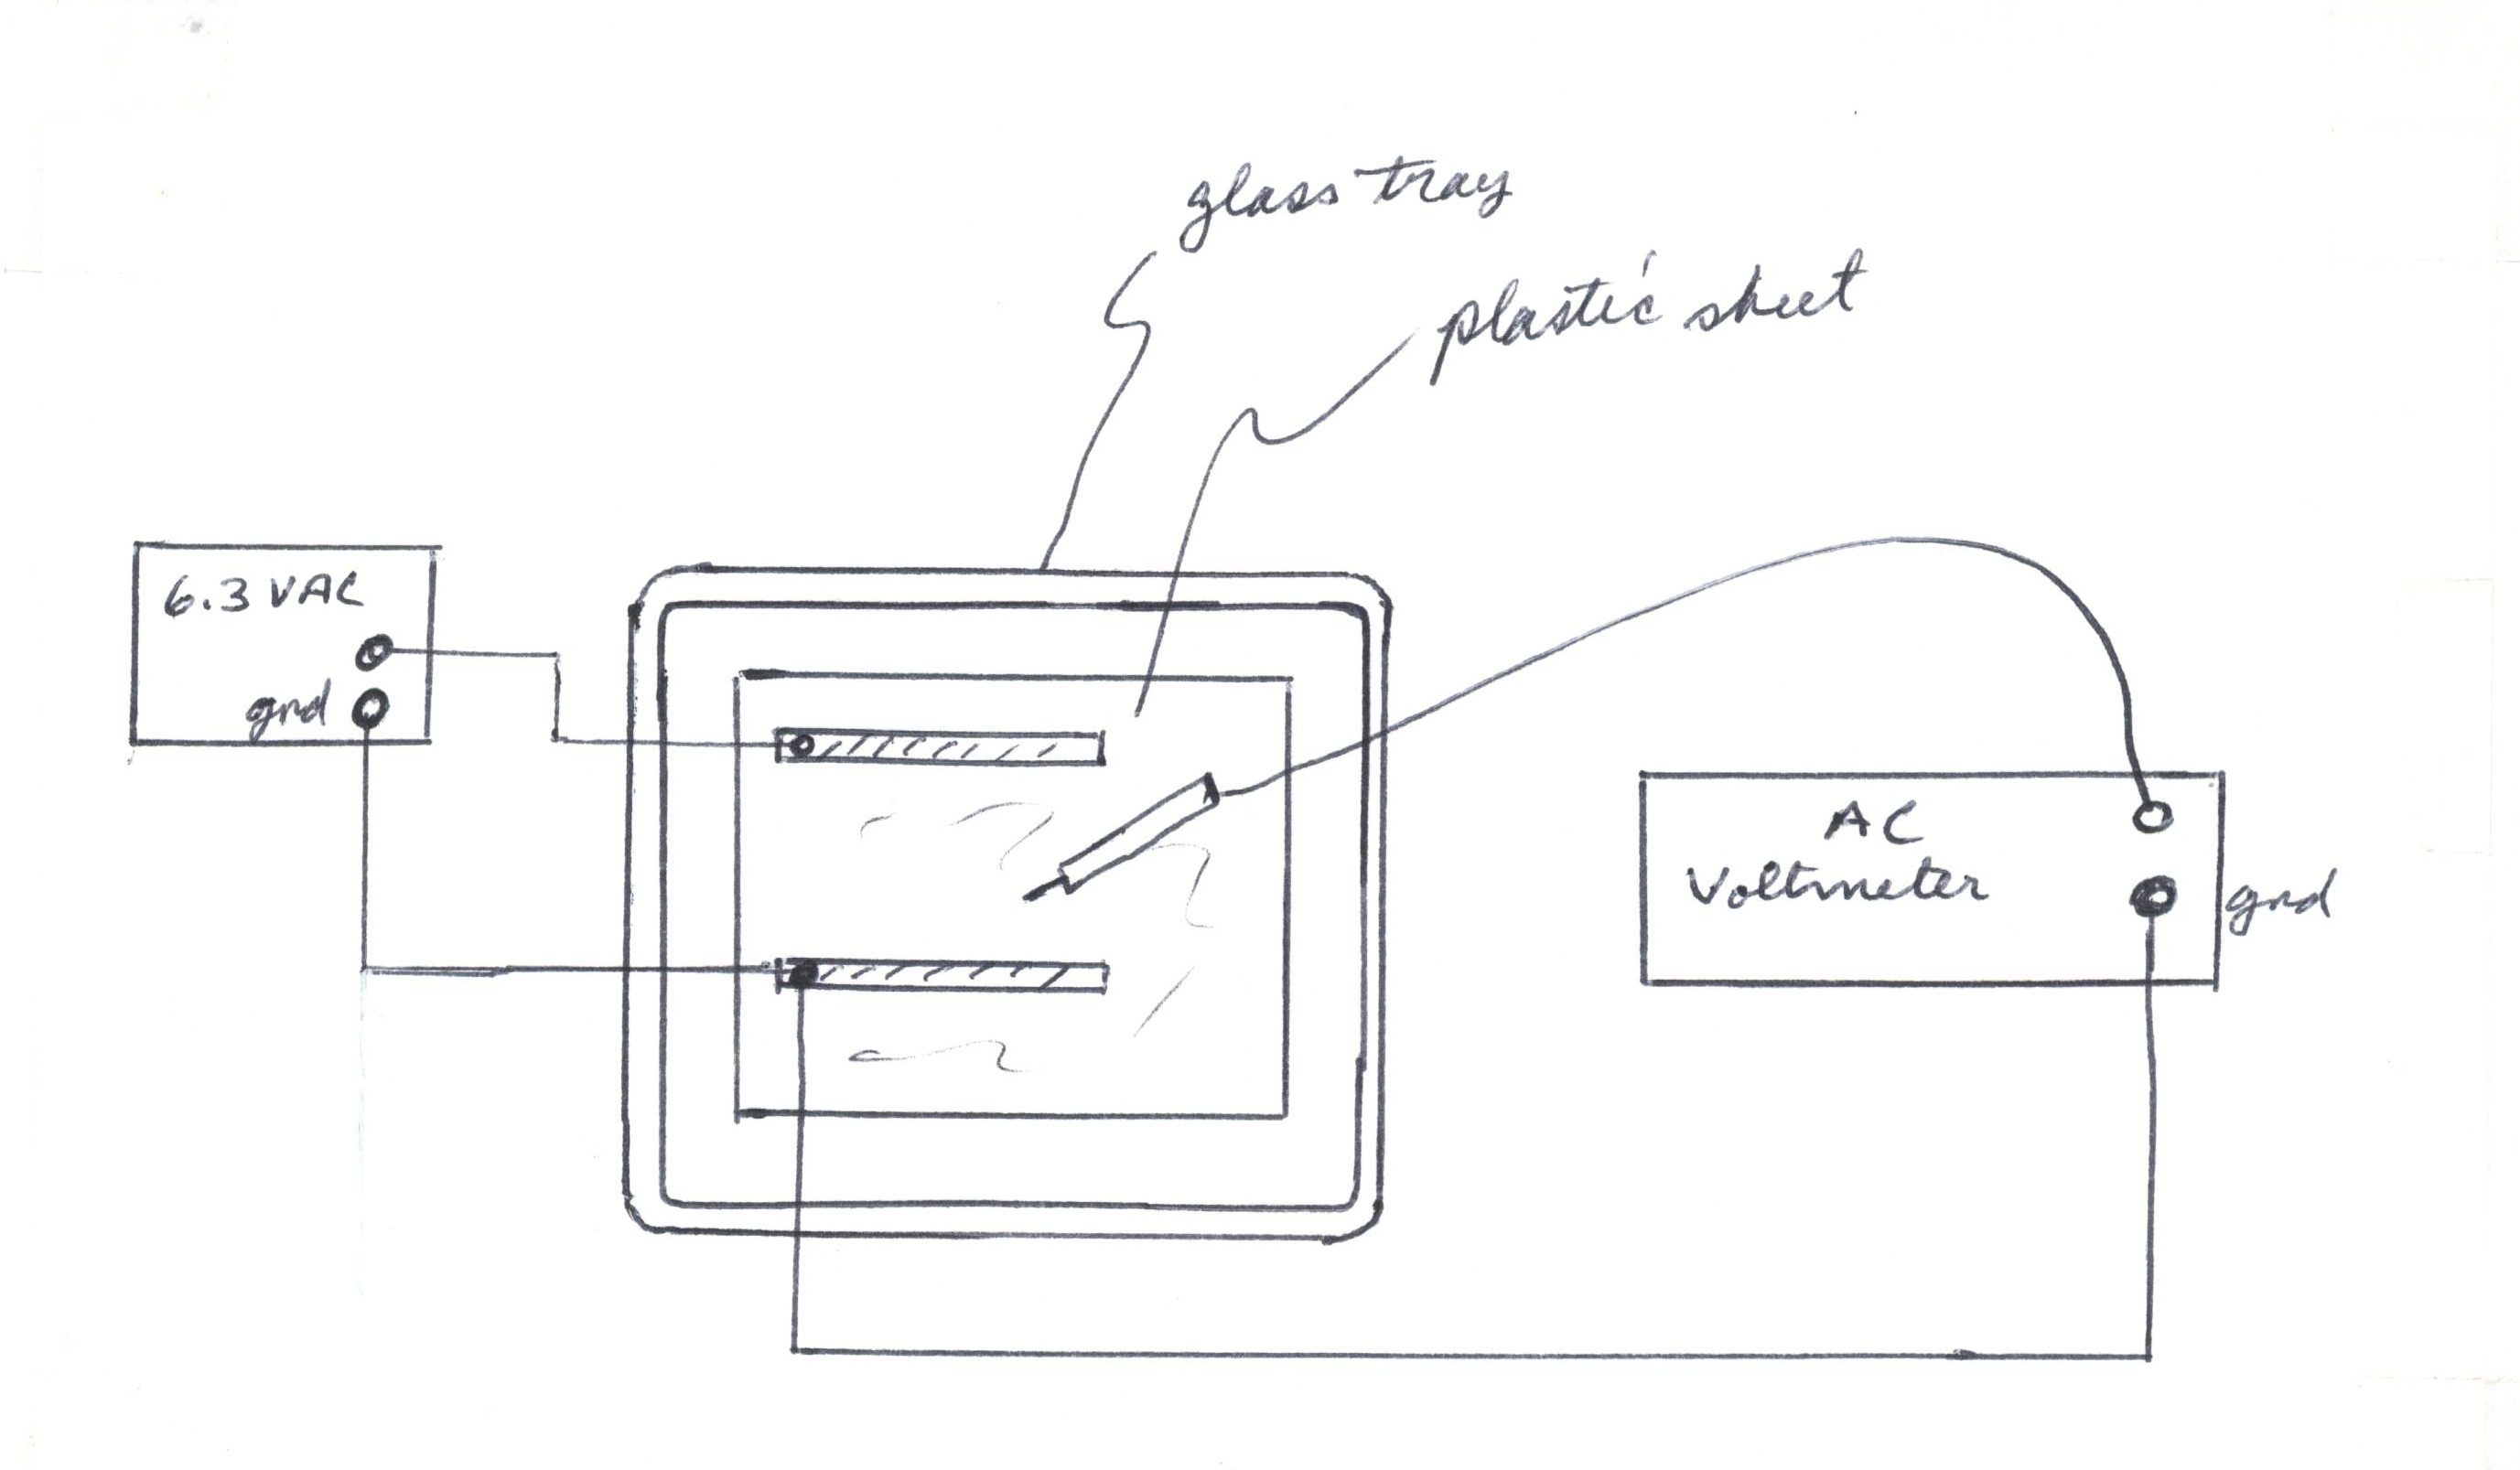
\includegraphics[scale=0.5]{5bgraf/fig_1}
%	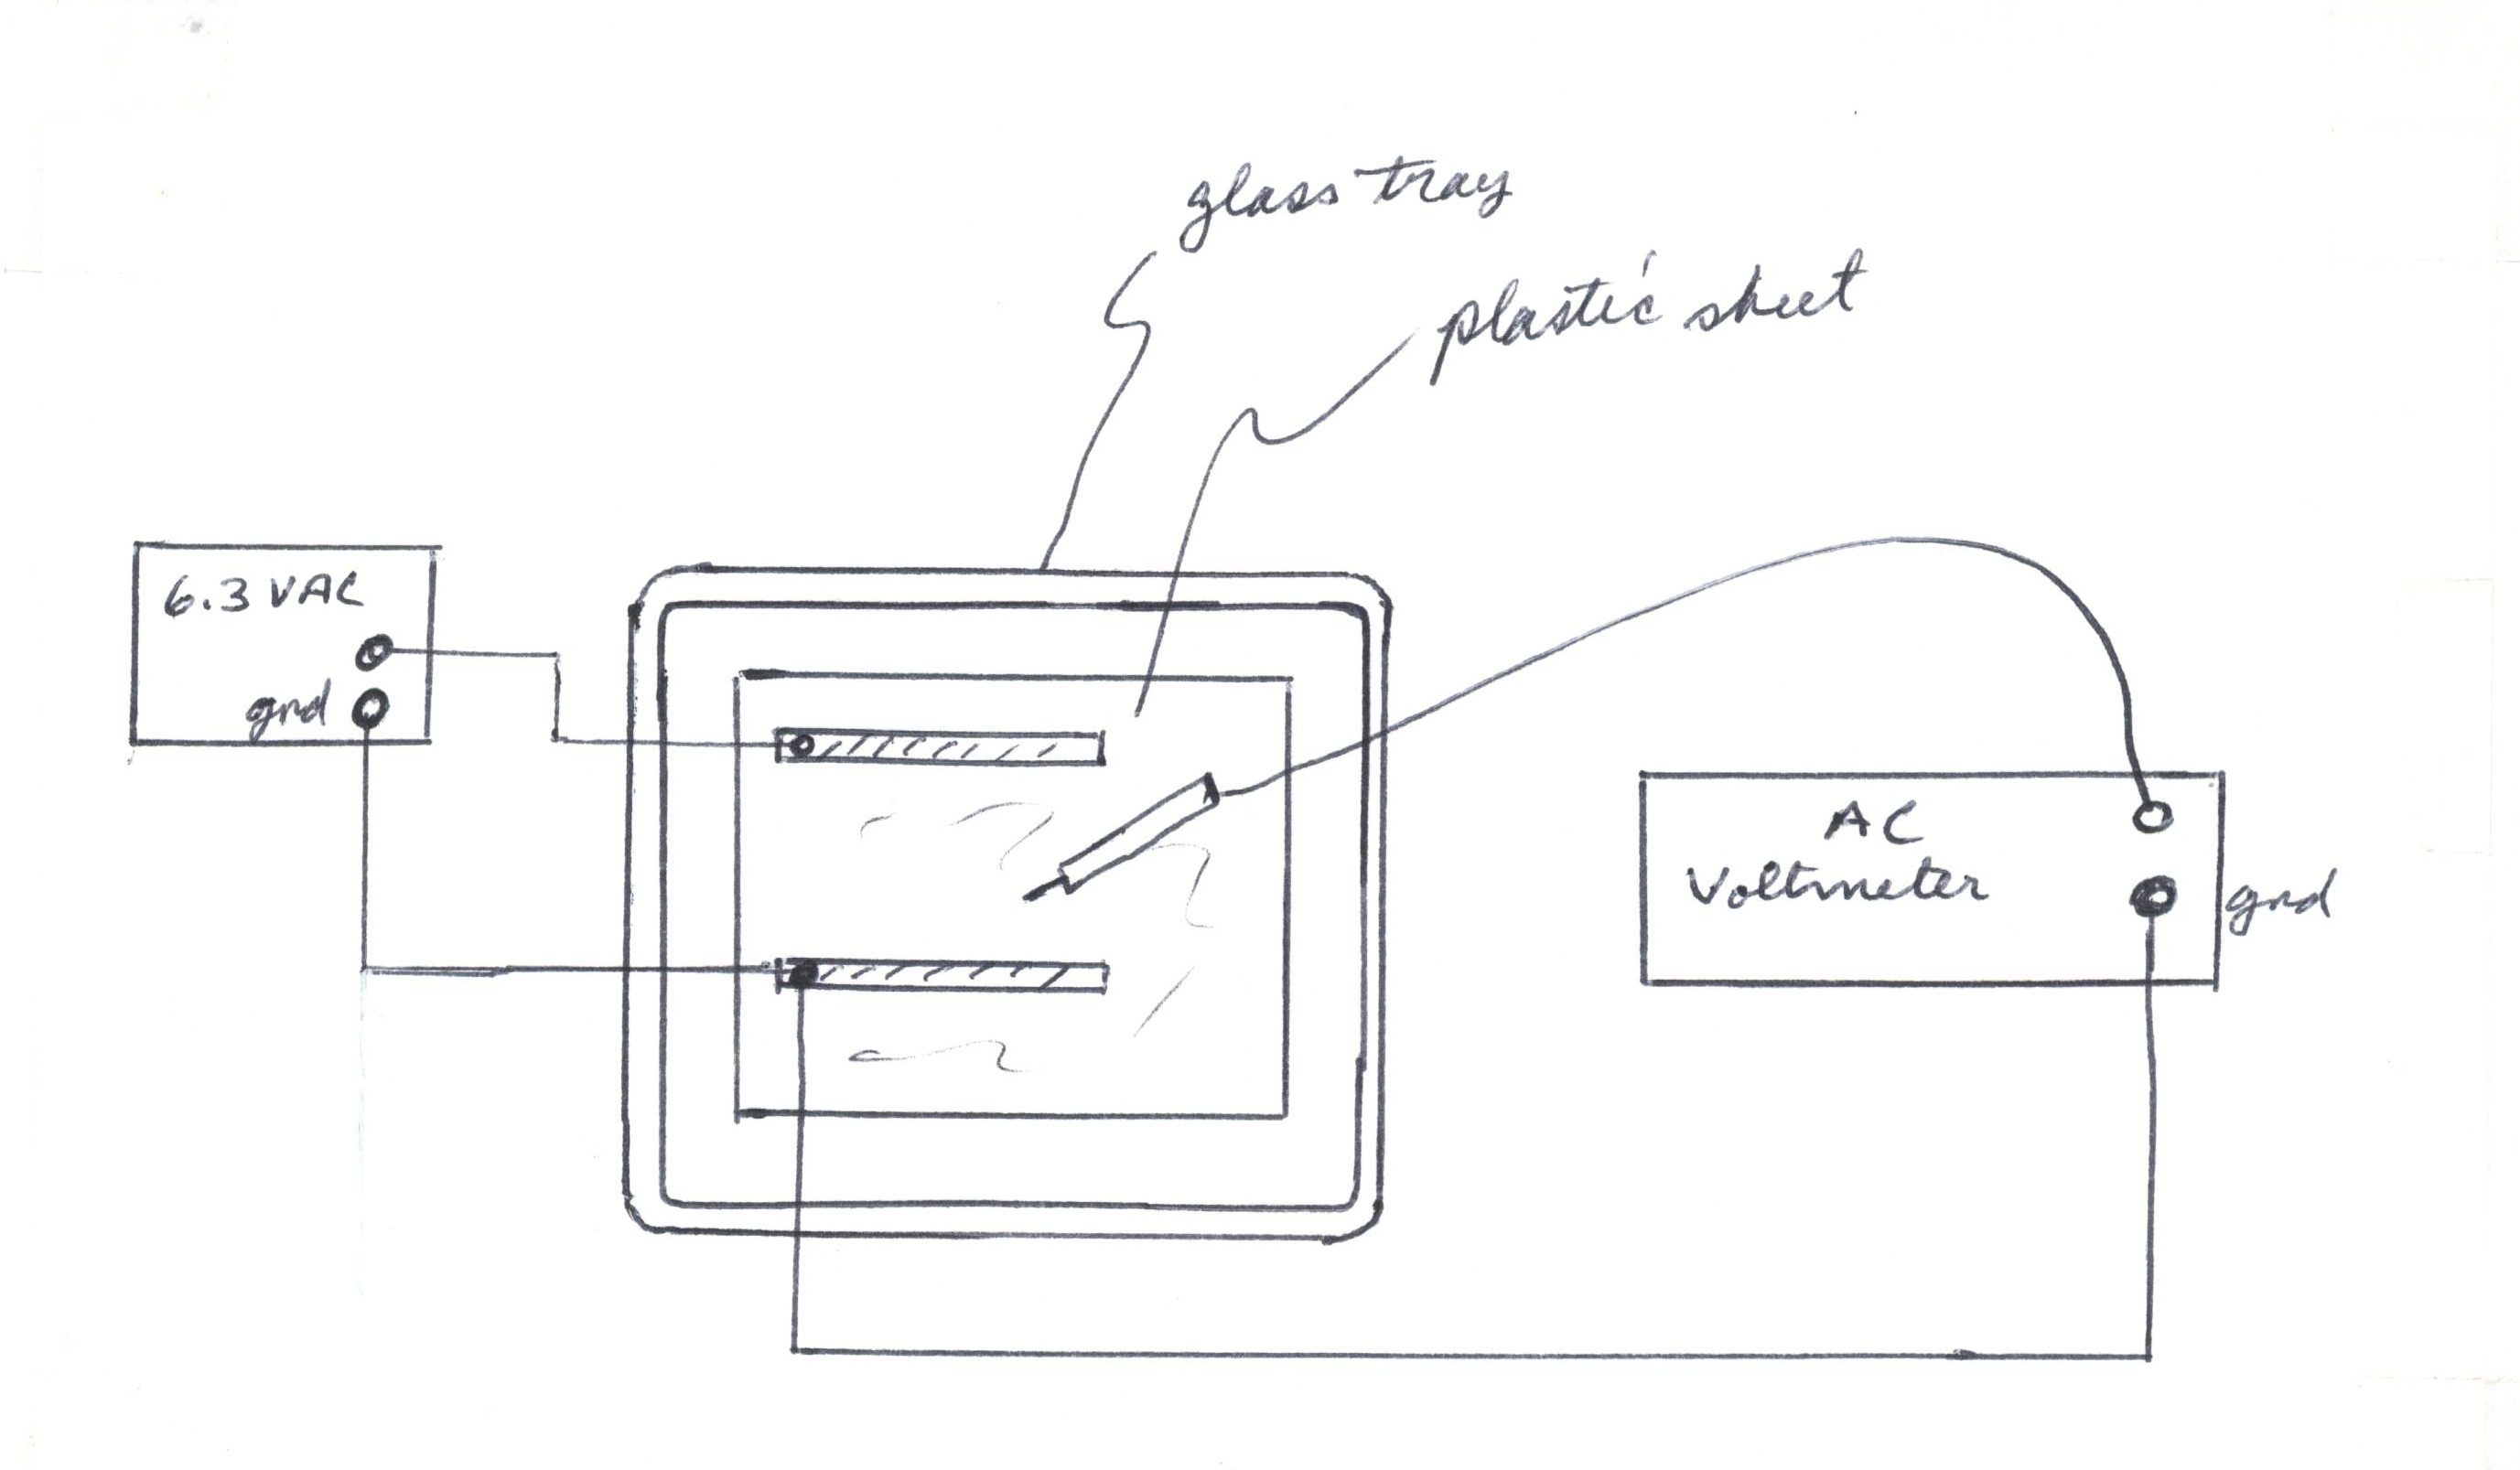
\includegraphics[bb = 20 0 400 200]{5bgraf/fig_1}
%	\caption{This simulation of charged plates allows you to map the electric potentials and determine the electric field between the plates.}
	\mfcaption{This simulation of charged plates allows you to map the electric potentials and determine the electric field between the plates.}
	\label{f:fig1}
%\end{figure}
\end{center}

\subsection{Activity: Parallel plates} %\label{s:plates}
\begin{enumerate}
	 \item Set up the two parallel bars as shown in \reffig{f:fig1} to simulate the potentials and fields surrounding parallel plates.
	 \item  Take data on a clear plastic sheet taped to the bottom of the tray.  Do this by finding locations of identical voltage and then dimpling (making small depressions) the plastic with the AC voltmeter probe.  
	 The dimples are not very visible under water but once you have measured four or five representative constant voltages (you should make note of the voltages separately), remove and dry the plastic sheet and the dimples will be easily seen.  
	 Use the provided marker pens to connect dots of equipotential (constant voltage), thereby determining equipotential lines.
	  \item Draw electric field lines using the rules for the relationships between them and equipotential lines discussed in the text. Essentially, the two lines are perpendicular to each other at every point.
	 \item Calculate the value of the electric field between three (3) different potential pair values inside the plates and at one (1) potential pair value outside the plates, and one (1) point in the ``fringe'' area using \refeqn{e:EandV}. For example, between the plates:\\[5pt] 
\[
	E = \frac{V_2 - V_1}{d_2 - d_1} = \frac{(4.0 - 2.5) \text{ V}}{(2.5 - 1.1)\text{ cm}}= 1.07 
	\frac{\text{V}}{\text{cm}}
\]

\begin{center}
\begin{tabularx}{\linewidth}{>{$}X<{$}>{$}X<{$}>{$}X<{$}} % p{35pt} for text col of 35pt
	\hline
	\Delta V \text{ (V)}&\Delta d \text{ (m)} & E \text{ (V/m)}\\
	\hline
	1.5 & 0.014 & 107 \\ 
\end{tabularx}
\mtcaption{Electric field values}
\end{center}


	\item Discuss and document (write down) your observations regarding whether the equipotential and field lines have the shapes and behaviors you would expect for this geometry.
%	\item Be prepared to show your field plot to the class using the overhead projector and also to explain your observations and analysis to the class.
\end{enumerate}

\subsection{Activity: Circular electrodes}
Repeat the activities under parallel plates for two small round electrodes that simulate point charges. Calculate the value of the electric filed between two (2) distinct locations.

\subsection{Activity: Other configurations}
Repeat the activities under parallel plates for a more creative configuration. Calculate the value of the electric filed between two (2) distinct locations.
\end{multicols}

\section{Questions}
\begin{enumerate}
	 \item Explain what aspects of these measurements contributed to experimental uncertainties.
	 \item Include an estimate of how much uncertainty there is in the measurements of voltage and position and whether these resulted in a departure of your experimental results from expected outcomes.
\end{enumerate}

%\newpage
%\includegraphics*[width=\textwidth,trim=120 80 80 120,clip]{5bgraf/pslabgrid} 

%---------------------------------------------------------------------
\endinput
%---------------------------------------------------------------------
			%--lab 02-------------------------------------
 
%--------------------------------------------------------------------------
% !TEX root = 5Blman.tex
% energy.tex
% 2012.12.27 changed to 2col format
%--------------------------------------------------------------------------
\chapter{Electric Energy}

%---------------------------------------------------------------------
\begin{multicols}{2}
\section{Purpose}
  The purpose of this laboratory exercise is to explore the relation between electrical energy and heat. You will find the energy transferred to a cup partially filled with water with a current passing through it.  The energy will be found using calorimetry methods and compared to electrical methods.  This lab will help you to understand concepts of energy and power associated with electric current and demonstrate the conversion of electrical energy to heat. You will also be able to describe what is meant by joule heat, explain the factors on which joule heat depends, and show how joule heat may be measured experimentally. The heat generated or power dissipated is referred to as joule heat.

%The purpose of this laboratory exercise is to describe what is meant by joule heat, explain the factors on which joule heat depends, and show how joule heat may be measured experimentally
\section{Preparation}
  Reread the sections in your text regarding electrical energy and power before coming to lab. Pay special attention to the relationship of voltage, current, and power.  You may also wish to review sections in your text on temperature change and specific heat.
%\paragraph{Short quiz }
% Be prepared to take a short quiz or hand in a prelab assignment at the beginning of lab related to the concepts of voltage, current, power, and energy.

%---------------------------------------------------------------------
\section{General Information}
Using your measured values of mass, temperature, voltage, current, and time you will calculate the energy put into a cup partially filled with water and associated material around it.  The energy will be calculated by two methods.  First by considerations of the energy needed to cause a temperature change and second by considerations of electrical energy.  The results of the two calculations should agree within experimental uncertainties if most or all of the energy put into the system by the electric current is retained as thermal energy in the system.  We thus verify that the energy associated with temperature change is the same as the energy associated with electric current. 
 \reffig{f:fig2} shows the basic set-up.  A DC power supply is connected to a coil of wire immersed in an aluminum cup partially filled with water.  (Not shown are the cup's lid, the stirring device, and the thermometer.)  The current is passed through an ammeter connected in series with the coil.  The voltage across the coil is measured by a voltmeter. %connected as shown.  
\paragraph{Caution}
Be sure you understand the operation of the various components in the circuit.  Do not turn on the power supply until the instructor has checked to see that the system is wired correctly.  The ammeter is particularly vulnerable to damage if improperly connected.  Also, do not turn on the current unless the heating coil is immersed in water or it may burn out or burn you.

\begin{center}
%\begin{figure}
%	\centering
	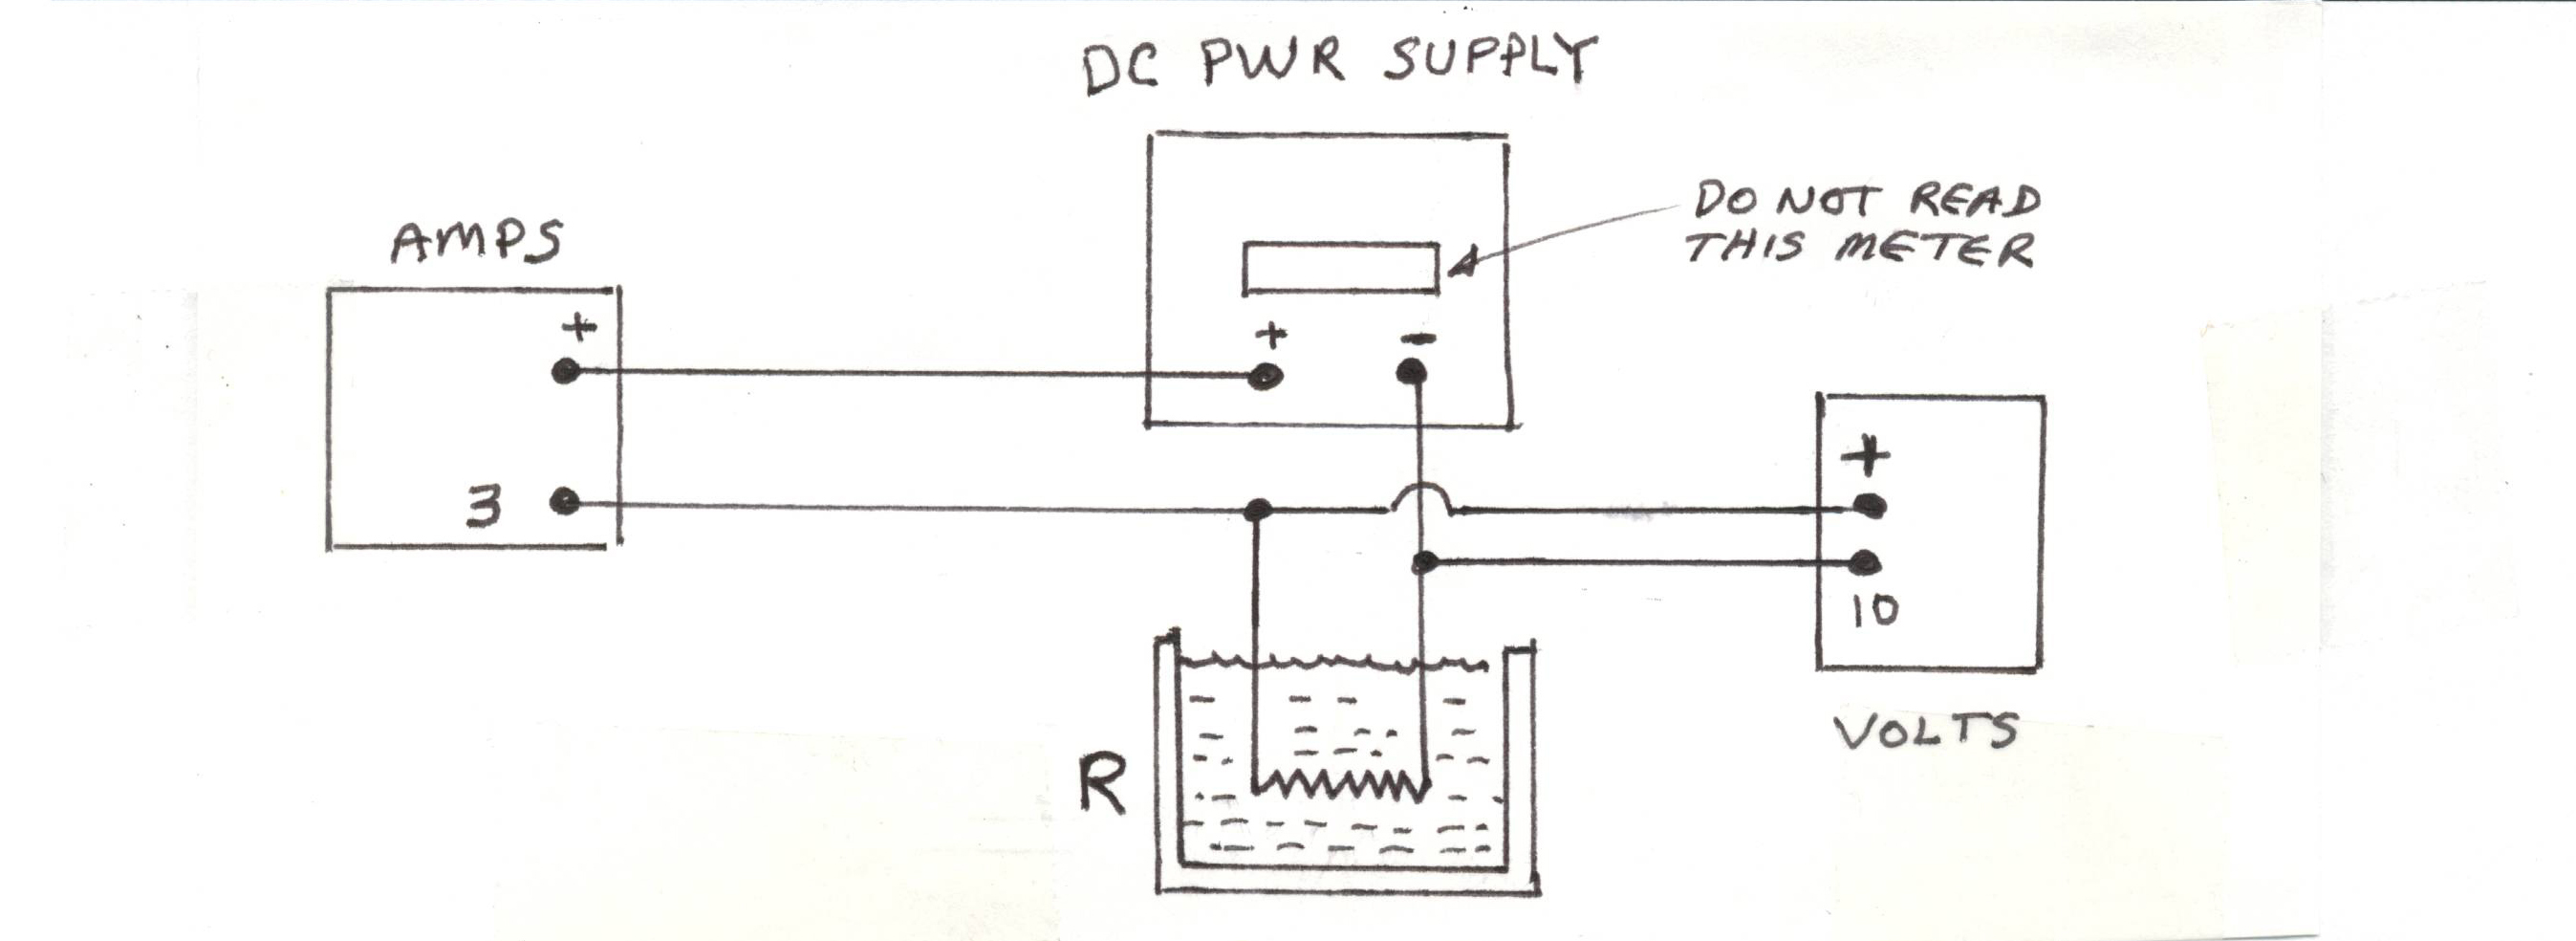
\includegraphics[scale=0.65]{5bgraf/fig_2}
%	\caption{Block diagram for calorimetry set-up}
	\mfcaption{Calorimetry set-up: block diagram}
	\label{f:fig2}
%\end{figure}
\end{center}

%\begin{center}
%	\includegraphics[scale=0.8]{5bgraf/fig_2b}
%	\mfcaption{Calorimetry set-up: schematic}
%	\label{f:fig3}
%\end{center}

%---------------------------------------------------------------------
\section{Theory}
To calculate the energy needed to heat the system by the calorimetry method we note that the amount of energy needed to increase the temperature of an object is
\begin{equation} \label{e:qheat1}
	Q = mc\Delta T 
\end{equation}
where $Q$ is the amount of heat, $m$ is the mass of the object, $c$ is its specific heat, and $\Delta T$ is the change in temperature, $\Delta T =T_2 - T_1$.  Since our system has more than one substance, the energy required is the sum of the energy needed for each substance in the system.

In this exercise we heat water in an aluminum cup.  But we also heat the coil of wire, stirrer, thermometer, and part of the lid and connecting rods.  This sounds complicated, but experimentation has determined that all of these other factors are equivalent to 6.00 cal/\si{\degree}C of water. Finally, we assume that everything that is heated has the same temperature change.  Therefore, the equation we use to calculate the energy input by the calorimetry method is
\begin{equation}\label{e:qheat2}
	Q = [m_wc_w + m_{Al}c_{Al} + m_{coil}c_{coil}](T_2 - T_1)
\end{equation}
where	
\begin{description}[itemsep=1pt]
	\item [$m_w$] = mass of water
	\item [$m_{Al}$]	= mass of Al calorimeter cup
	\item [$c_w$]	= specific heat of water (1.00 cal/g \si{\degree}C)
	\item [$c_{Al}$]	= specific heat of Al (0.22 cal/g \si{\degree}C)
	\item [$m_{coil}c_{coil}$] $\approx$ (6.00 cal/\si{\degree}C) = experimental \\estimate for heating coil
	\item [$T_2$]	= final temperature
	\item [$T_1$]	= initial temperature
\end{description}

%\vskip{6pc}
To calculate the electrical energy supplied by the current, $I=q/t$ note that the electrical energy, $E = W$ is: %the product of power and time ($E = Pt$), electrical power is the product of current and voltage ($P = IV$), so that electrical energy is:

\begin{equation}\label{e:iheat} E = W = qV = (It)V = IVt\end{equation}
which represents the energy expended or the work done in a circuit in a time  $t$ across a potential difference or voltage $V$.	

%\begin{description}[itemsep=1pt]
%	\item[$I$] 	= electric current
%	\item [$V$] = voltage
%	\item [$t$] = time (from turn on to turn off voltage)
%\end{description}

Then the power is 
\begin{equation}\label{e:power} P = W/t = IV \end{equation}

Apply this to a resistance $R$, the heating coil in our case, the expended energy or work done becomes

\begin{equation}\label{e:eWork} 
E = W = IVt = I^2Rt = \frac{V^2t}{R} 
\end{equation}

The electrical energy expended takes the form of heat energy and is commonly called \textsl{joule heat} or \textsl{$I^2 R$} losses, the power or energy expended per unit time.

By conservation of energy
\begin{align} 
\text{electrical energy expended} & = \text{heat gained} \notag \\
W & = Q \notag \\
IVt & = mc\Delta t \notag
\end{align}
or
\begin{equation}
IVt = [m_wc_w + m_{Al}c_{Al} + m_{coil}c_{coil}](T_2 - T_1)
\end{equation}

Thus in both the calorimetry and the electrical methods you will make calculations of energy based on simple physical measurements.  You will need to keep notes on the measurements to estimate their uncertainties.  The two methods should agree within experimental uncertainties.

%---------------------------------------------------------------------
\section{Activities}
Set up the equipment as shown in the block and schematic diagrams.  Ask your instructor to check the wiring before proceeding.  Estimate the uncertainty in each measured value and write a brief justification for each estimate. Perform two separate runs using ``fresh'' water in the calorimeter.

\subsection{Calorimetric and electrical measurement}

Measure and record the mass of the aluminum cup when empty and dry.
Add cold water until the cup is about \slashfrac{3}{4} full, then measure and record the mass again.

Assemble the calorimeter cup, insulating disk, and metal jacket and insert the heating coil, stirrer, and thermometer.  Be sure that the heating coil is completely submerged below the water surface and is a few degrees below room temperature. Allow the system to come to an equilibrium temperature and then record the initial temperature.

Prepare to take measurements of the time, temperature, voltage, and current and record the values in a table. Also, plot the temperature vs. time as you proceed so you can get a `visual' determination of when the system reaches equilibrium.

Turn on the power supply and start the timer once you have quickly adjusted the current to 2.2A.  You may have to adjust the power supply occasionally to keep the current constant at 2.2A.  Record both the current and the voltage during the experiment.  Stir the water and take temperature readings every 30 seconds until the temperature of the system has risen at least \ang{11}~C to \ang{15}~C above its initial starting value.  Turn off the power supply, but continue to take temperature measurements %for an additional 2 minutes with power off. 
until a maximum temperature is reached. Record this temperature as $T_2$, the final temperature.

Compute the heat energy (in calories) gained by the calorimeter system using \refeqn{e:qheat2} to complete the calorimetry method. %associated with the temperature increase. Also, convert the value in calories to Joules. 

Compute the electrical energy (in Joules) your readings of current, voltage, and time (in seconds) using  \refeqn{e:iheat} for the electrical energy  method.

Then compute the ratio of the electrical energy to the heat energy to determine the ``electrical equivalent of heat'' in \emph{J/cal} or \emph{J/kcal}. Compare the result to the accepted value of the mechanical equivalent of heat by comparing the percent uncertainty or percent error, given by
\[ \frac{|Expt. - Std. value|}{Std. value} \times 100\% \]
 The standard accepted value is, 1~cal = 4.186~J.

%Find the percent difference between the two calculations and discuss whether they agree within estimated experimental uncertainties.
\end{multicols}
%---------------------------------------------------------------------
\section{Questions}
\begin{itemize}
	\item Determine the uncertainties in reading the voltmeter, ammeter, thermometer, and the balance scale.
	\item For a constant current, $I$, how is the joule heat related to the resistance of the heating coil?
	\item Which method (calorimetry or electric) should be inherently more precise?  Why is this so?
	\item What do your graphs of temperature versus time tell you about the assumption that the energy put into the system is retained as thermal energy?
	\item If the cost of electricity were \$0.12 per kWh, what is the cost of electricity in cents per kJ used for this experiment?
\end{itemize}

%--------------------------------------------------------------------------
\endinput
%--------------------------------------------------------------------------
			%--lab 03-------------------------------------

%--------------------------------------------------------------------------
% !TEX root = 5Blman.tex
% dc1.tex
% 2013.01.06 changed to 2col format
%--------------------------------------------------------------------------
\chapter {DC Circuits Part I}

%---------------------------------------------------------------------
\begin{multicols}{2}
\section{Purpose}  
The purpose of this laboratory exercise is to explore series and parallel connections of resistances as well as series and parallel connections of emfs.  More importantly, you will practice the measurement and calculation of voltage, current, resistance, and power in simple circuits.

%---------------------------------------------------------------------
\section{Preparation}  
Read the material in your textbook regarding resistance, voltage, current, and simple DC circuits before coming to lab. Pay special attention to the major features of resistors in series and parallel and to the associated problem-solving strategies for them.

%---------------------------------------------------------------------
\section {Short quiz}  Be prepared to take a short quiz at the beginning of lab related to the concepts of series and parallel connections of resistors and emfs.

%---------------------------------------------------------------------
\section{General Information}
You will use three different methods to find resistance.  In the first you will simply use a color code to ``read'' the resistance value from the resistor markings. In the second method, you will the use an ohmmeter (one of the functions provided by a multimeter) to measure resistance directly.  In the third method you will use instruments to measure voltage across and current through a resistor, then calculate the resistance using Ohm's law --- this process is  referred to as ohm's method.

\begin{equation} R = V/I \label{e:ohm} \end{equation}

% \paragraph {You will calculate and measure the resistance of series and parallel connections of resistors.}  

Within experimental uncertainties the ohmmeter readings and the ohm's law measurements should be consistent.  Your instructor will inform you what error analysis to perform and direct you regarding how to report your results.

In series the total or equivalent resistance $R_S$ is 

\begin{equation} \label{e:ser}
	R_S  =  R_1  +  R_2  +  R_3  + \cdots	
\end{equation}

For resistors in parallel, the total or equivalent resistance $R_P$ is

\begin{equation} \label{e:par}
	%1/R_P  =  1/R_1  +  1/R_2  +  1/R_3  + \cdots
	R_P  =  \left (1/R_1  +  1/R_2  +  1/R_3  + \cdots \right)\relax^{-1}
\end{equation}

\paragraph {Color codes.}Some resistors are marked with colored bands to indicate the resistance they had at the time of manufacture.  Although reading the color code does not constitute a measurement of resistance which may have changed over time by usage, it is useful to see what the nominal resistance should be.  The first and second colored bands give the first and second digits of the resistance.  The third band gives the power of ten and the fourth band indicates the precision of the manufactured resistance:  5\% for gold and  10\% for silver.

For example, if the bands are red, blue, green, and gold, the resistance is $26 \times 10^5\,\Omega$ with 5\% precision.

%\begin{table}
%\caption{Resistor Color Code}
%\centering
%\begin{tabular}{l c l c}Color & \# & Color & \# \\
%\hline
%Black	&	0 &	Green	& 5\\
%Brown	&	1 &	Blue	& 6\\
%Red		&	2 &	Violet	& 7\\
%Orange	&	3 &	Gray	& 8\\
%Yellow	&	4 &	White	& 9\\
%\end{tabular}
%\end{table}
%
%\begin{center}
%%\begin{tabularx}{\linewidth}{>{$}X<{$}>{$}X<{$}>{$}X<{$}}
%\begin{tabularx}{\linewidth}{XcXc}Color & \# & Color & \#}
%	\hline
%	Black	&	0 &	Green	& 5\\
%	Brown	&	1 &	Blue	& 6\\
%	Red		&	2 &	Violet	& 7\\
%	Orange	&	3 &	Gray	& 8\\
%	Yellow	&	4 &	White	& 9\\
%\end{tabularx}
%\mtcaption{Electric field values}
%\end{center}

\begin{center}
\begin{tabularx}{\linewidth}{@{}XXXc@{}}
	\hline
	Color	& \# & Color	& \# \\
	\hline
	Black	&	0 &	Green	& 5\\
	Brown	&	1 &	Blue	& 6\\
	Red		&	2 &	Violet	& 7\\
	Orange	&	3 &	Gray	& 8\\
	Yellow	&	4 &	White	& 9\\
\end{tabularx}
\mtcaption{Resistor Color Code}
\end{center}

\paragraph{Warning}  Your instructor will describe the operation of the instruments -- electronic multimeter, voltmeter, and ammeter.  Ammeters are instruments used to measure current and are particularly vulnerable to damage.  Have your instructor check your connections the first time you measure current to be certain that the meter is arranged correctly so that it is not damaged. The multimeter has a very low resistance when measuring current --  this allows the meter to be placed in series and not significantly change the resistance of the circuit.  The ammeter is placed in series so that it has the full current of the circuit branch passing through it.  This also makes the ammeter vulnerable to high currents and subsequent damage if it is connected directly to a voltage source.

%---------------------------------------------------------------------
\section {Measuring resistance}
These activities center on measuring resistance using three different methods. (1) Read the color code to get the value of a resistor. (2) Measure the resistor with an ohmmeter to get  its resistance value. (3) Measure voltage across and current through a resistor, then calculate the resistance value --- this process is  referred to as ohm's method.

%\begin{figure}[htb]
%	\centering
%	\includegraphics[scale=0.6]{5bgraf/mohm} %{5bgraf/fig_3}
%	\caption{Single resistor connected to an ohmmeter}
%	\label{f:mohm}
%\end{figure}

\begin{center}
	\includegraphics[scale=0.6]{5bgraf/mohm} %{5bgraf/fig_3}
	\mfcaption{Single resistor connected to ohmmeter}
	\label{f:mohm}
\end{center}

\subsection{Activity: Ohm's law} \label{s:ohmlaw}
\begin{enumerate}
	\item \label{l:mm} Determine the individual resistances of three different resistors using the multimeter as indicated by \reffig{f:mohm}.
	
	\item \label{l:olm}Determine the resistances by the Ohm's law method in which applied voltage and current are measured and the resistance is calculated using \refeqn{e:ohm}.  The block diagram in \reffig{f:mamblock} indicates how to set up these measurements.

	\item Make a table of the voltages and currents measured in item \ref{l:olm} and the resistances calculated from them.  Also list the measured values of resistance found directly with the multimeter from item \ref{l:mm} and those determined from the color code so that you can make side-by-side comparisons.
	
%\begin{center}
\begin{tabularx}{\linewidth}{@{}lllll@{}}
	\hline
	V(V)	& I(mA) & $R_{calc}$(\si{\ohm})	& $R_{msrd}$(\si{\ohm}) & $R_{code}$(\si{\ohm}) \\
	\hline
\end{tabularx}
\mtcaption{Ohm law method comparisons}
%\end{center}


	\item Estimate the percent uncertainties in the voltage and current measurements and calculate the percent uncertainty in the resistances found in item \ref{l:olm} with the Ohm's law method.  Do the resistances found by the three different methods for each resistor agree with one another within these experimental uncertainties? If not, discuss why they might disagree.
	
	%\item Find the percent difference between the values of resistance found in item \ref{l:olm} and measurement by ohm's law and color code values. Discuss whether the values agree within experimental uncertainties.  If not, discuss why they might disagree.
	% This section can be confusing to read. Essentially, students are checking how direct measurement with an ohmmeter compares with current and voltage measurement followed by a calculation of resistance. This can also be compared with a direct rendering from the color code.
\end{enumerate}

%\begin{figure}[htb]
%	\centering
%	\includegraphics[scale=0.8]{5bgraf/mamblock} %{5bgraf/fig_4}
%	\caption{Measurement of current through and voltage across a resistor}
%	\label{f:mamblock} %{f:fig4}
%\end{figure}

\begin{center}
	\includegraphics[scale=1]{5bgraf/mohmLaw}%{5bgraf/mamblock} %{5bgraf/fig_4}
	\mfcaption{Schematic for Ohm's law measurement}
	%{Measurement of current through and voltage across a resistor}
	\label{f:mamblock} %{f:fig4}
\end{center}

\subsection{Activity: Resistances in series} \label{s:series}
\begin{enumerate}
	\item \label{l:eqs} Determine the equivalent resistance of each resistor connected in series using the Ohm's law method. To do this measure the voltage across each resistor separately and the current through it. The current is the same through each resistor. The schematic in \reffig{f:mamblock} shows the measurement of the voltage across and the current through a single resistor. Use  \reffig{f:serpar}. to measure the voltages and current for multiple resistors in series.
	
	\item Once you have measured the voltage and current for each resistor separately, calculate the equivalent series resistance $R_S$ using \refeqn{e:ohm}.
	
	\item Determine the experimental uncertainty in the value of $R_S$. %found in item \ref{l:eqs}.
	
	\item Calculate the equivalent resistance $R_S$ using \refeqn{e:ser} where the individual resistances are those found by the Ohm's law method.
\end{enumerate}

%\begin{figure}
%	\centering
%	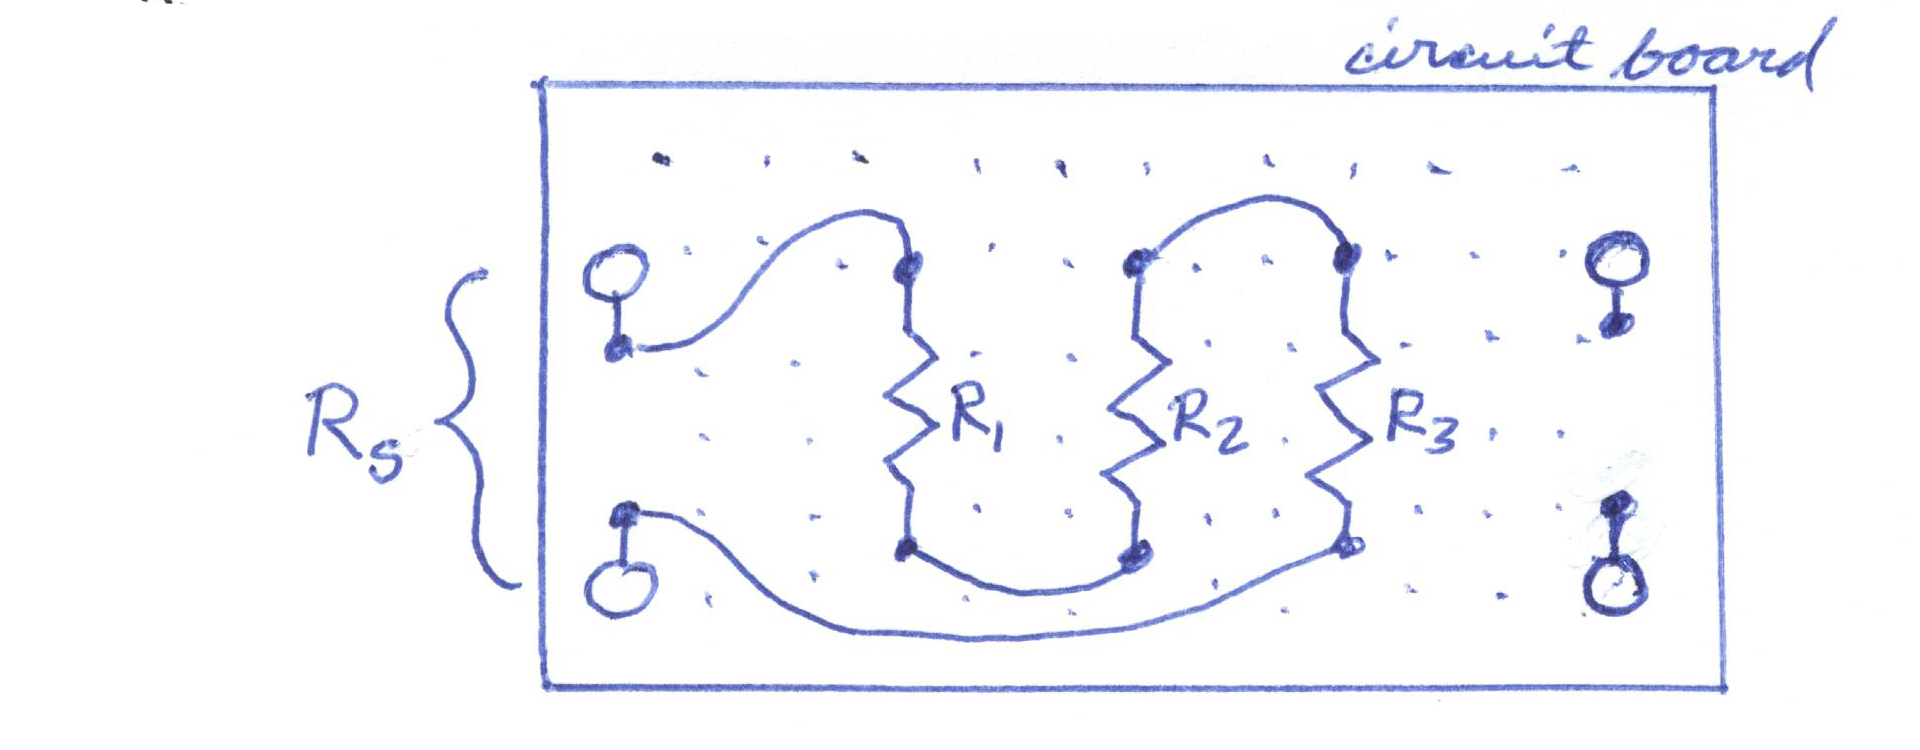
\includegraphics[scale=0.8]{5bgraf/fig_5}
%	\caption{Resistors in series}
%	\label{f:fig5}
%\end{figure}

%\begin{figure}[htb] \centering
% \subfloat[series circuit]
%   {\includegraphics[scale=0.5]{5bgraf/r3series}\label{f:fig5}} % fig_5
% \hfill
% \subfloat[parallel circuit]
%   {\includegraphics[scale=0.5]{5bgraf/r3parallel}\label{f:fig6}} % fig_6
% \caption{Resistors in series and parallel}\label{f:serpar}
%\end{figure}

\begin{center}
   {\includegraphics[scale=1]{5bgraf/r3series2}
   \label{f:r3series}} % fig_5
% \vfill
	\vskip 0.5cm
   {\includegraphics[scale=1]{5bgraf/r3parallel2}
   \label{f:r3par}} % fig_6
 \mfcaption{Resistors in series and parallel}
 \label{f:serpar}
\end{center}


\subsection{Activity: Resistances in parallel}
\begin{enumerate}
	\item Determine the equivalent resistance of three resistors connected in parallel using the Ohm's law method.  Again, review \reffig{f:mamblock} to remind yourself how to measure voltage and current for a single resistor --- use \reffig{f:serpar} for voltage and current measurements of multiple resistors in parallel.
	
	\item Calculate the equivalent resistance $R_P$ using \refeqn{e:ohm} where the individual resistances are those found by the Ohm's law method.

	\item Once you have measured the voltage and current, calculate the equivalent parallel resistance $R_P$ using \refeqn{e:par}.
	
	\item Determine the experimental uncertainty in the value of $R_P$.
\end{enumerate}

%\begin{figure}
%	\centering
%	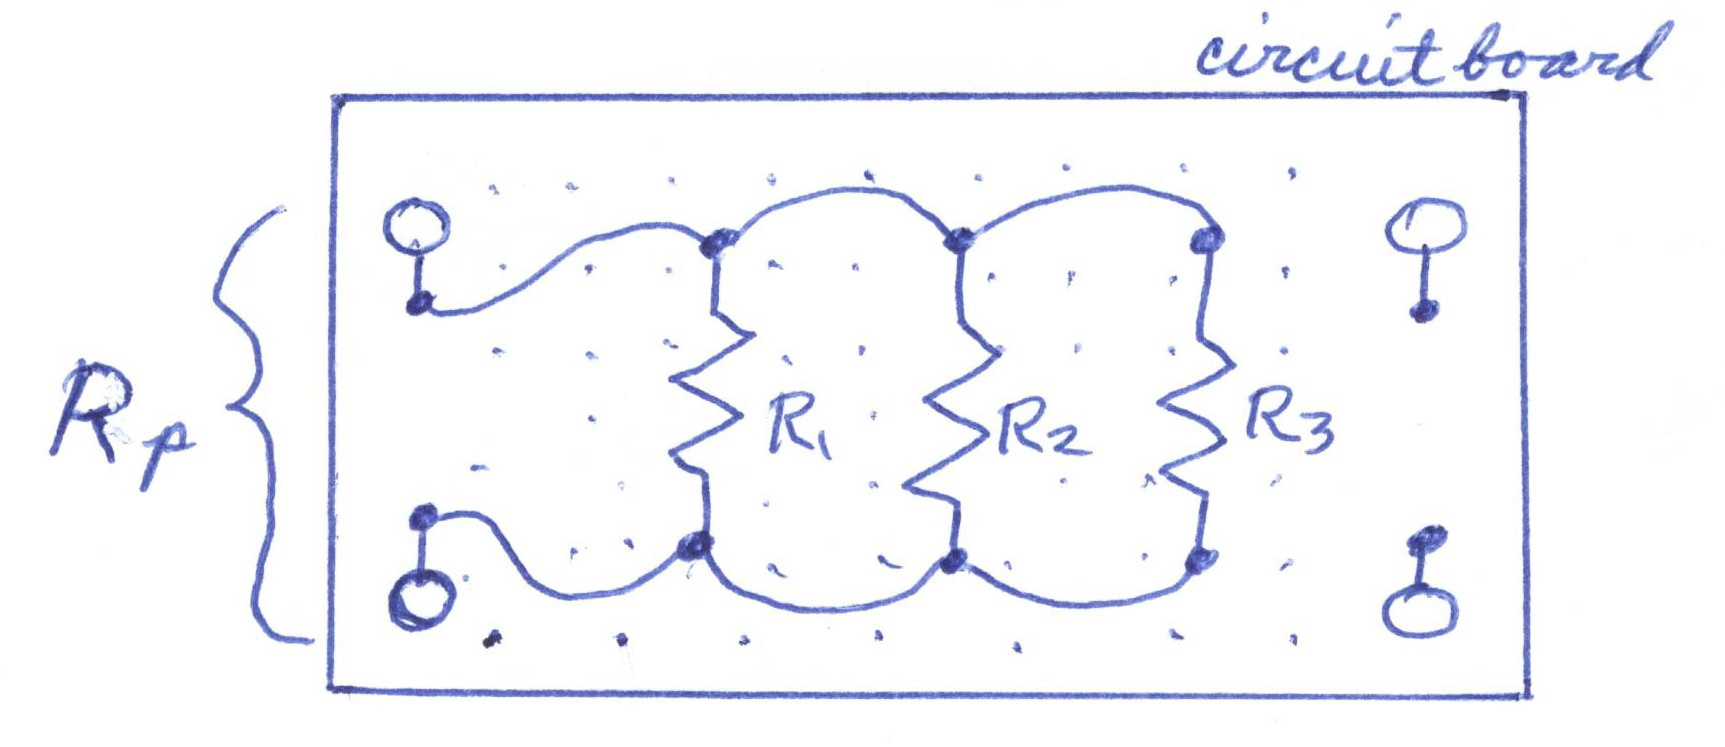
\includegraphics[scale=0.8]{5bgraf/fig_6}
%	\caption{Resistors in parallel}
%	\label{f:fig6}
%\end{figure}

\subsection{Activity: EMF's in series and parallel}
\begin{enumerate}
	\item Measure the emfs of two individual dry cells and the total emfs when they are placed in series and in parallel as shown in \reffig{f:vseriespar}.
	
	\item Explain the values obtained in the series and parallel connections.
	
	\item Do they agree with theory?  If not, could the internal resistance of the emfs be responsible for the disagreement or is it within experimental uncertainties?
\end{enumerate}

%\begin{figure}[htbp]
%	\centering
%	\includegraphics[scale=0.7]{5bgraf/mvoltswitch}
%	\caption{Measurement of single dry cell}
%	\label{f:mvoltswitch}
%\end{figure}
%
%
%\begin{figure}[htb]
%	\centering
%	\includegraphics[scale=.9]{5bgraf/vseriespar} %{5bgraf/fig_7}
%	\mfcaption{Battery configurations in series and parallel}
%	\label{f:vseriespar} %{f:fig7}
%\end{figure}

\begin{center}
	\includegraphics[scale=1]{5bgraf/mvSwitch}	%{5bgraf/mvoltswitch}
	\mfcaption{Measurement of single dry cell}
	\label{f:mvSwitch}
\end{center}

\begin{center}
	\includegraphics[scale=1]{5bgraf/vserpar} %{5bgraf/fig_7}
	\mfcaption{Batteries in series and in parallel}
	\label{f:vseriespar} %{f:fig7}
\end{center}


\paragraph{If time permits}  Using the set-up in \reffig{f:serpar}, measure the voltage drops across each of the three resistors and compare these with the terminal voltage of the dry cell.  Discuss the meaning of your results.

\end{multicols}

\endinput

%\clearpage
%%\newpage
%\includegraphics*[width=\textwidth,trim=120 80 80 120,clip]{5bgraf/pslabgrid} 

%--------------------------------------------------------------------------
\endinput
%--------------------------------------------------------------------------
				%--lab 04-------------------------------------

%--------------------------------------------------------------------------
% !TEX root = 5Blman.tex
% dc2.tex
% 2013.01.07 changed to 2col format
%--------------------------------------------------------------------------
\chapter {DC Circuits Part II}

\begin{multicols}{2}
%---------------------------------------------------------------------
\section {Purpose}  
The purpose of the first part of this laboratory exercise is to explore the internal resistance of an emf.  The purpose of the second part is to analyze a circuit that is not a simple combination of series and parallel connections.  You will measure currents in this circuit and compare the results to an analysis using Kirchhoff's rules.  The concepts of emf, terminal voltage, and internal resistance as well as Kirchhoff's rules are also explored in lecture, your text, and in homework questions and problems.  By exploring them in lab you will not only become more familiar with them, but also build your skills in the measurement and evaluation of voltage, current, and resistance.

%---------------------------------------------------------------------
\section {Preparation} Pay special attention in your text to the major features of terminal voltage and Kirchhoff's rules and to the associated problem-solving strategies for them.

\paragraph {Short quiz}  Be prepared to take a short quiz at the beginning of lab related to the concepts associated with this laboratory exercise.

%---------------------------------------------------------------------
\section {General Information}
\paragraph {Warning}  You are already aware that ammeters (meters used to measure current) are particularly vulnerable to damage.  If you are not certain that you have correctly connected your ammeter have your instructor check your connections before you close the switch(es) that apply voltage to the circuit.

%---------------------------------------------------------------------
\section {DC Circuits}

%\begin{figure}
%	\centering
%	\includegraphics[scale=0.6]{5bgraf/vimtr} %{5bgraf/fig_8}
%	\caption{Setup to measure internal resistance of a battery}
%	\label{f:vimtr}
%\end{figure}

\begin{center}
	\includegraphics[scale=1]{5bgraf/vimtr} %{5bgraf/fig_8}
	\mfcaption{Setup to measure internal resistance of a battery}
	\label{f:vimtr}
\end{center}

\subsection{Activity: Internal resistance of a battery}
\begin{enumerate}
	 \item Set up the circuit shown in \reffig{f:vimtr}.  Use a precision resistor for $R$ and estimate the current that will flow so that you can choose an appropriate scale for the ammeter.
	\item Measure and record the current and terminal voltage as accurately as possible: $V_T$ = the terminal voltage, $E$ = the $emf$, $I$ = the current, and $r$ = the internal resistance.
\begin{equation} \label{e:vterm}
	V_T  =  E -Ir 	%\quad \text{with E = emf voltage}	
\end{equation}
	\item Replace the precision resistor with one having a different resistance and repeat the measurements of current and terminal voltage.
	\item Calculate the internal resistance $r$ of the battery for each resistor. Measure the the emf of the battery with nothing connected to it, and measure $V_T$ for each resistor.  Are your values consistent?  If not, it may be that the internal resistance actually varies with load.
\begin{equation} \label{e:rintern}
	r  =  \dfrac{E - V_T}{I} = \dfrac{E - IR}{I}	%\quad \text{with E = emf voltage}	
\end{equation}

	\item Discuss these results and your observations regarding the internal resistance of your battery in your lab report.
\end{enumerate}


\subsection{Activity: Kirchoff's rules}
%\begin{figure}
%	\centering
%	\includegraphics[scale=0.7]{5bgraf/kvlr3}	 %{5bgraf/fig_9}
%	\caption{Multiloop circuit with 3 unknown currents}
%	\label{f:kvlr3}
%\end{figure}

\begin{center}
	\includegraphics[scale=0.6]{5bgraf/kvlr3}	 %{5bgraf/fig_9}
	\mfcaption{Multiloop circuit with 3 unknown currents}
	\label{f:kvlr3}
\end{center}

\begin{enumerate}
	 \item Measure the emfs of both of your batteries.  Assuming the voltmeter has high resistance, the emf, $E$ is the voltage you measure with the battery alone connected to the voltmeter.
	\item Assemble the circuit shown in \reffig{f:kvlr3}.
	See \reffig{f:circboard} for a pictorial representation of the circuit.
	\item Measure the terminal voltages of your batteries with both tap keys held down.
	\item Using the block diagram of \reffig{f:circboard} on page \pageref{f:circboard} as a guide, measure the currents $I_1$, $I_2$, and $I_3$, --- remove the appropriate wire, insert the ammeter, then measure the current.
	\item Apply Kirchhoff's junction rule to junction $A$ and Kirchhoff's loop rule to the top and bottom loop.  Enter the values of the currents, resistances, and voltages for this circuit into each equation.  Are the rules verified by your values? Discuss your results.
	\item Solve the three equations obtained from the application of Kirchhoff's rules for the currents $I_1$, $I_2$, and $I_3$, treating them as unknowns. (Your instructor can provide some guidance in how to solve three equations for three unknowns.)
	\item Then calculate the currents using the known values of the resistances and voltages.  Compare the calculated values of the currents to the measured values and discuss how well they agree. 
\end{enumerate}

%\begin{figure} \centering
% \subfloat[circuit board]
%   {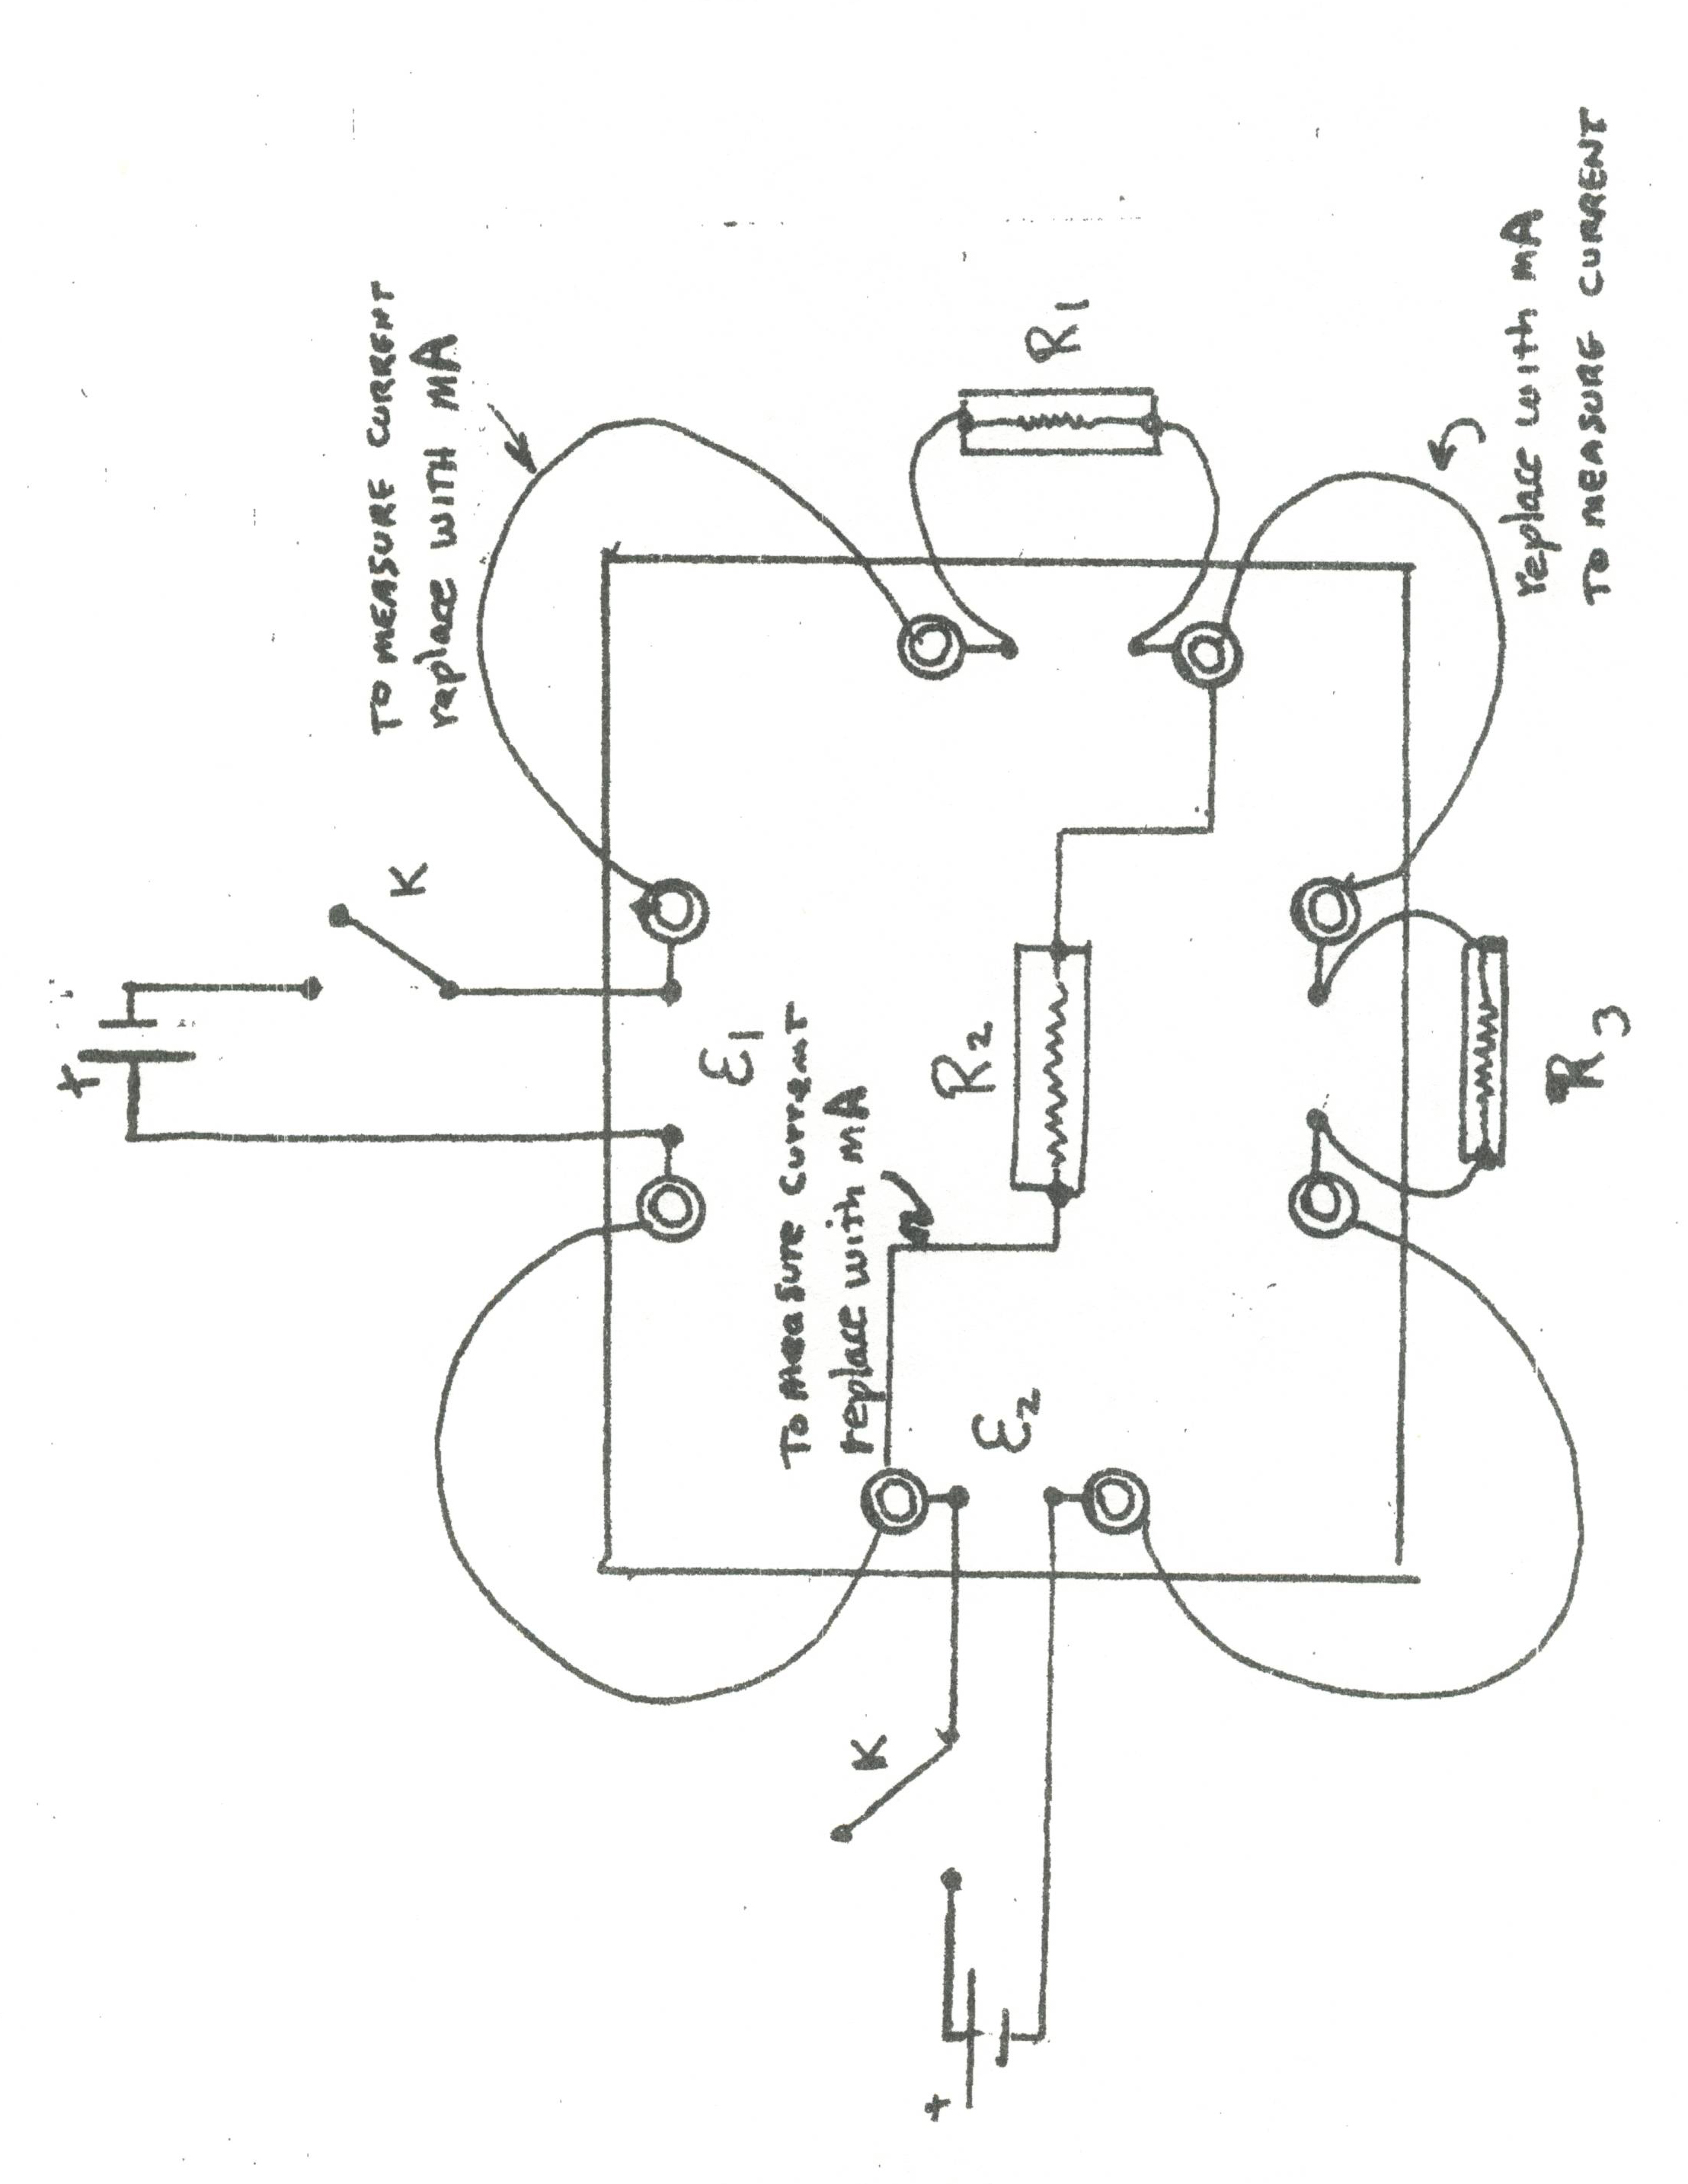
\includegraphics[scale=0.9]{5bgraf/fig_10b}\label{f:fig10b}}
%
% \subfloat[multimeter]
%   {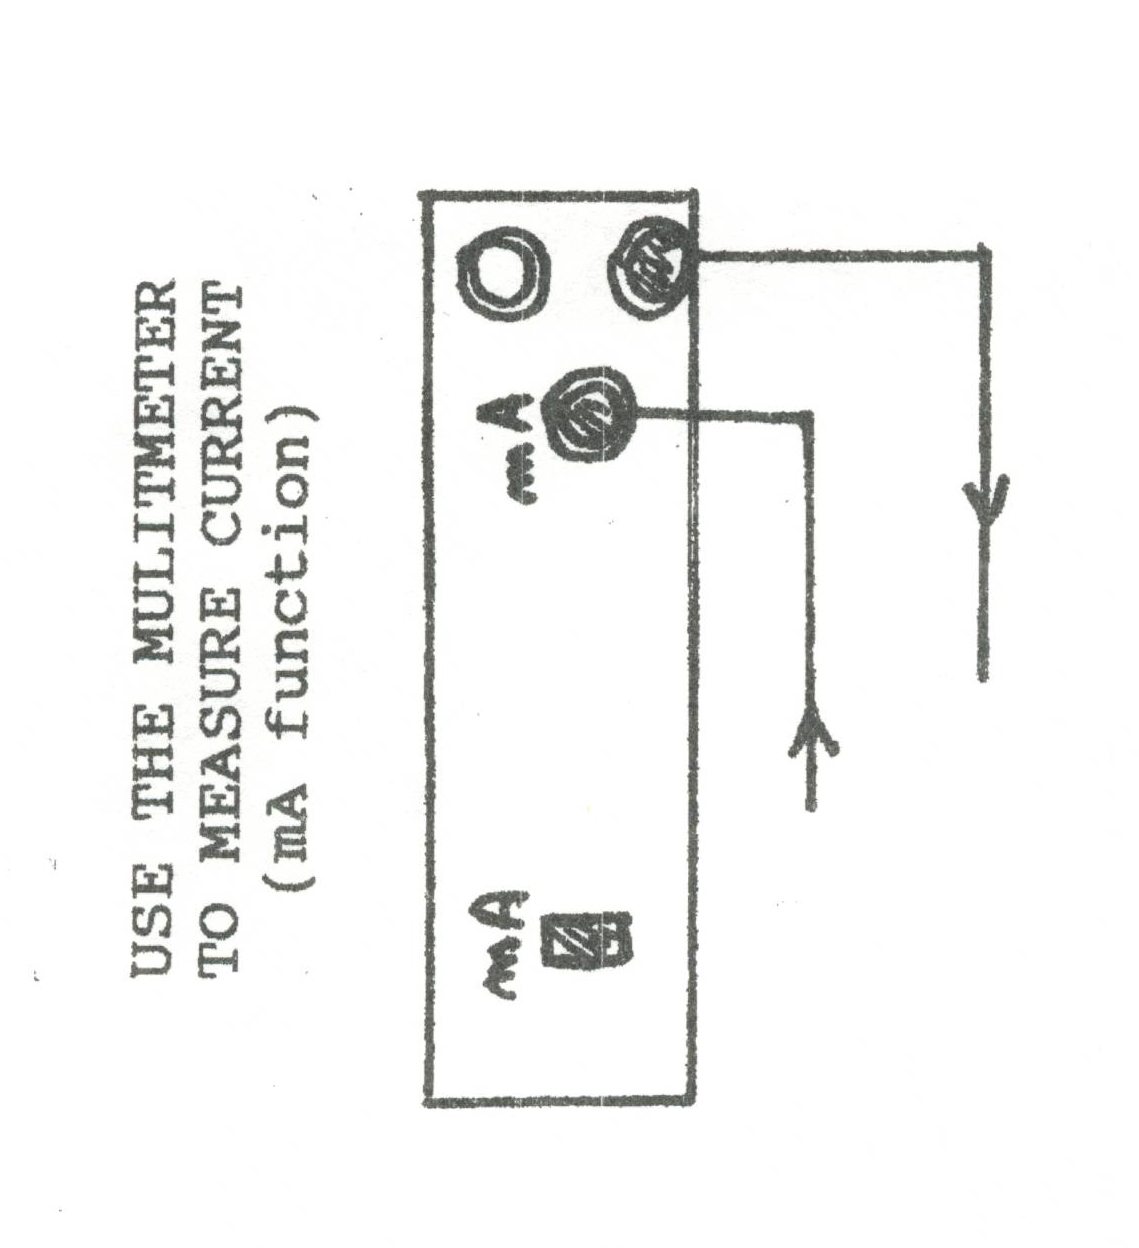
\includegraphics[scale=0.4]{5bgraf/fig_10a}\label{f:fig10a}}
% \caption{Circuit board arrangement for Kirchoff's rules}\label{f:circboard}
%\end{figure}
\end{multicols}

\begin{center}
   {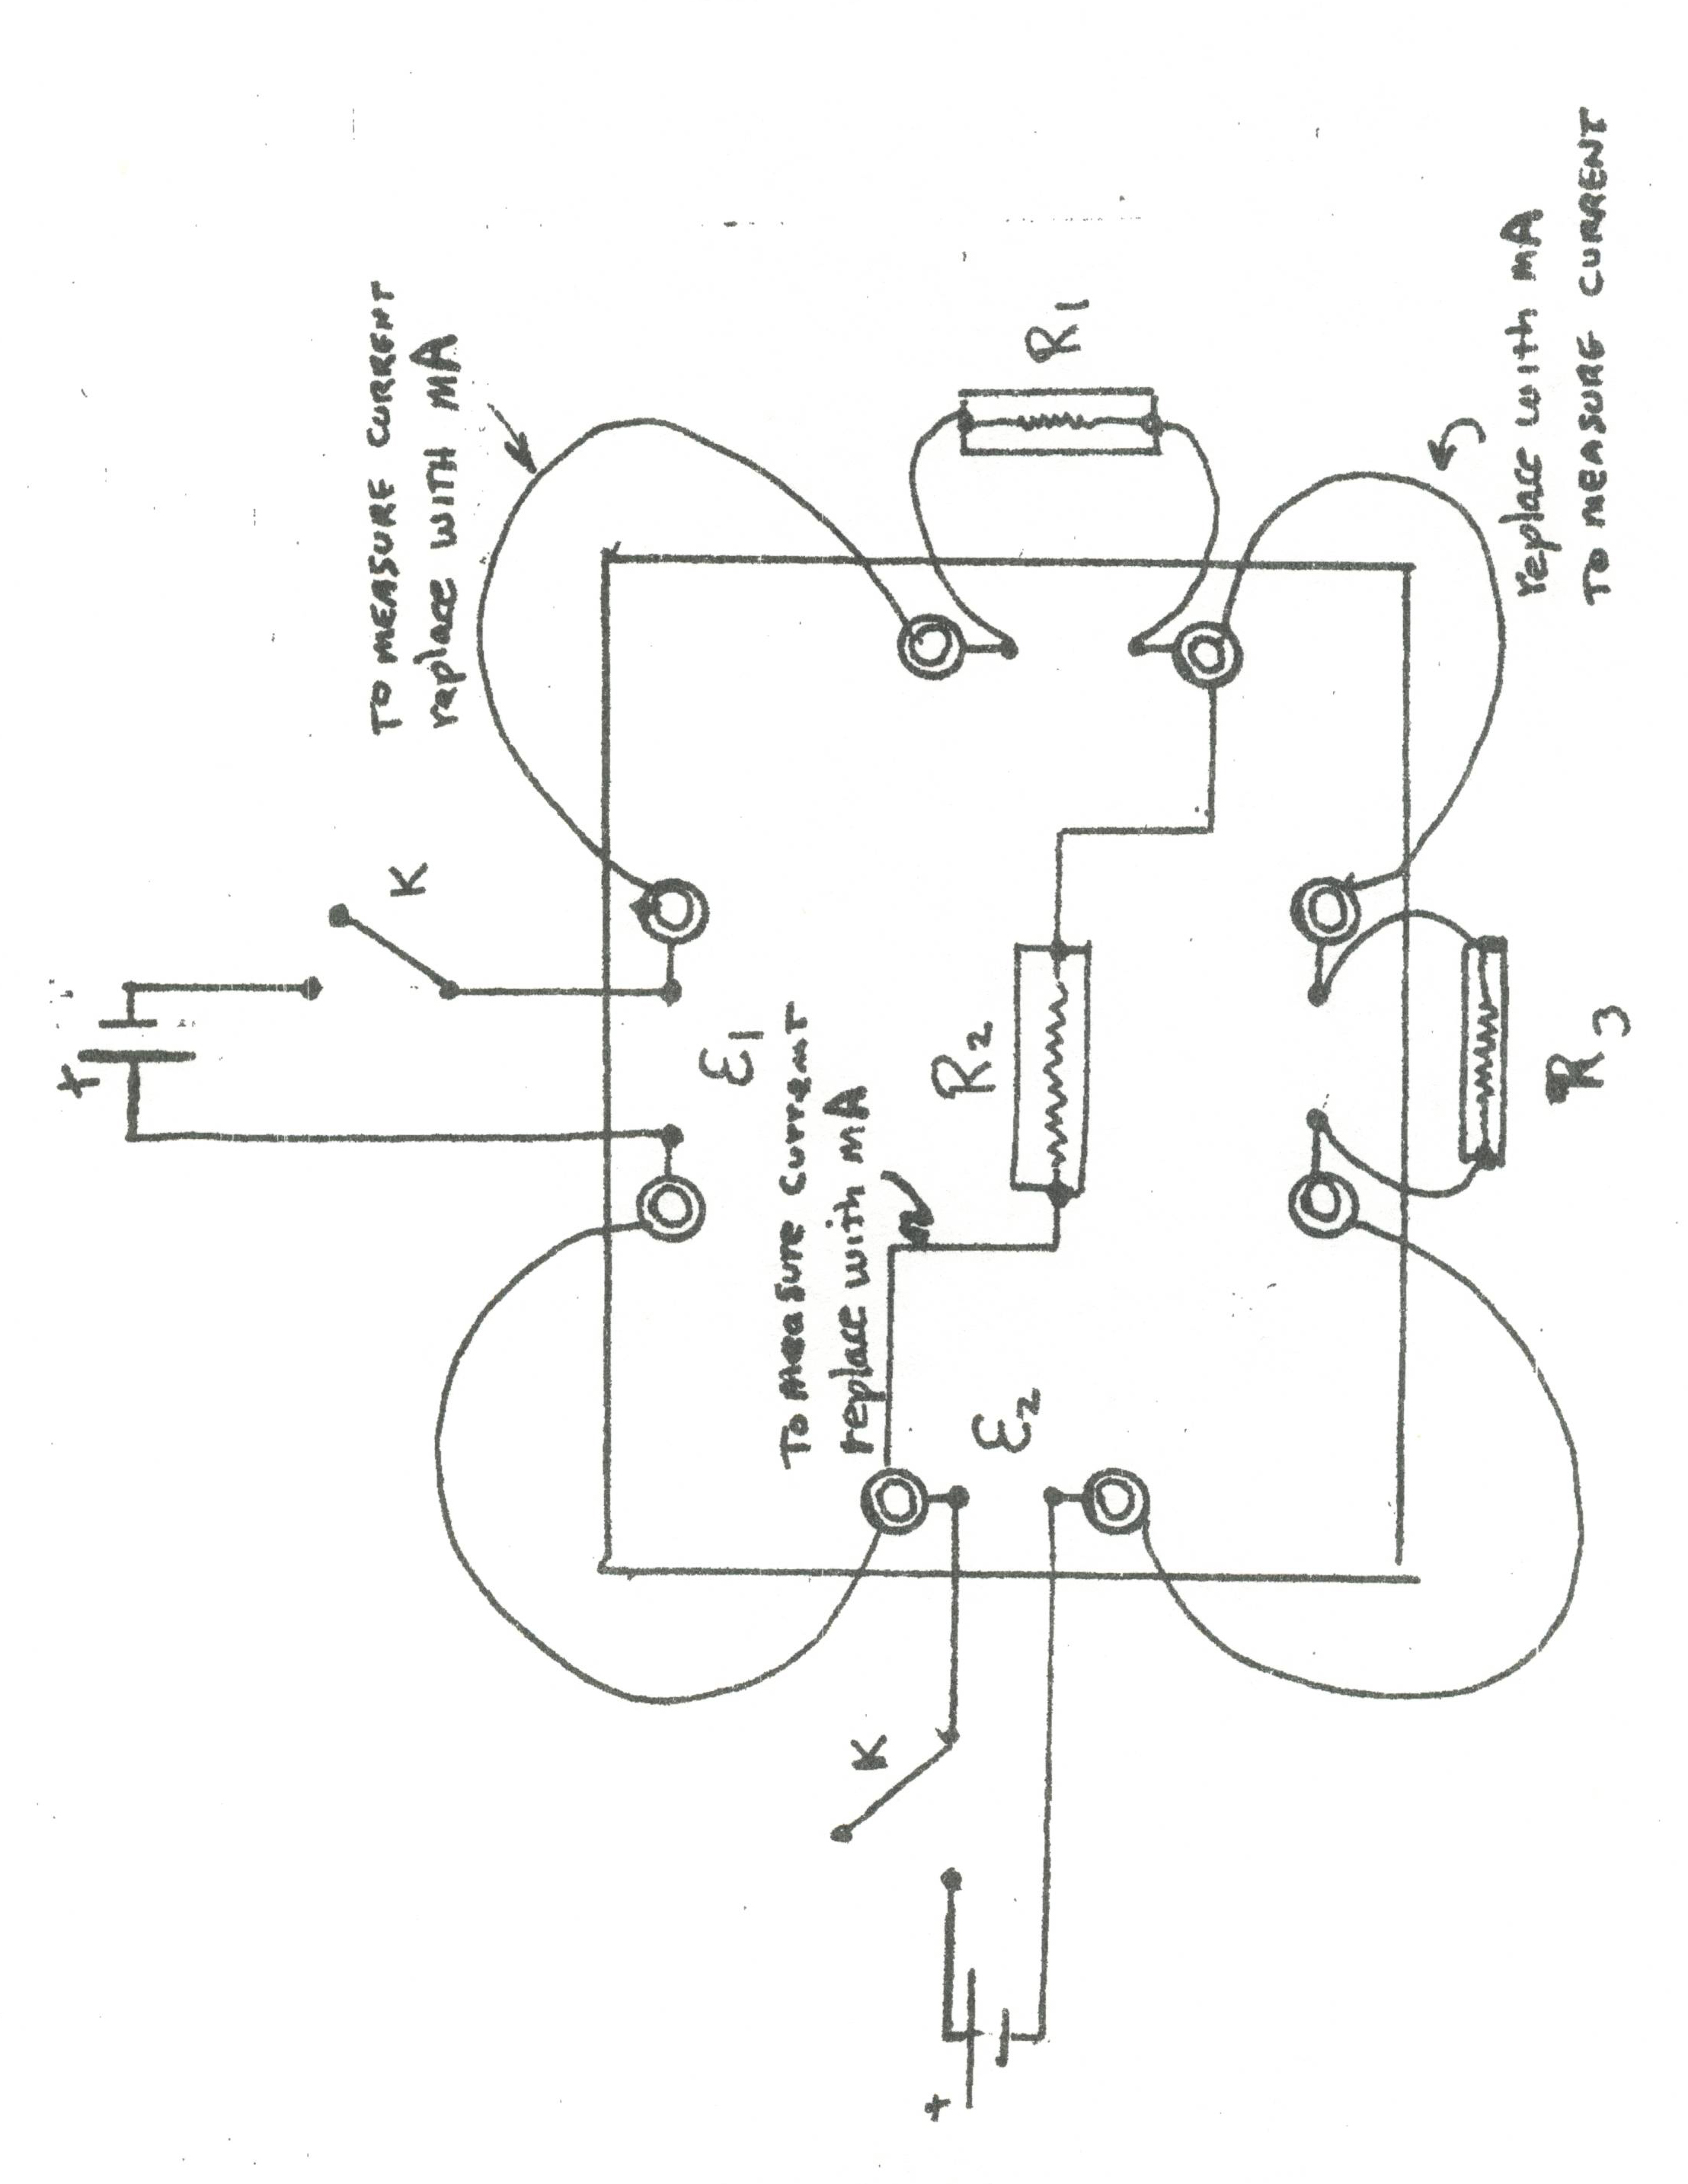
\includegraphics[scale=0.9]{5bgraf/fig_10b}\label{f:fig10b}}
   {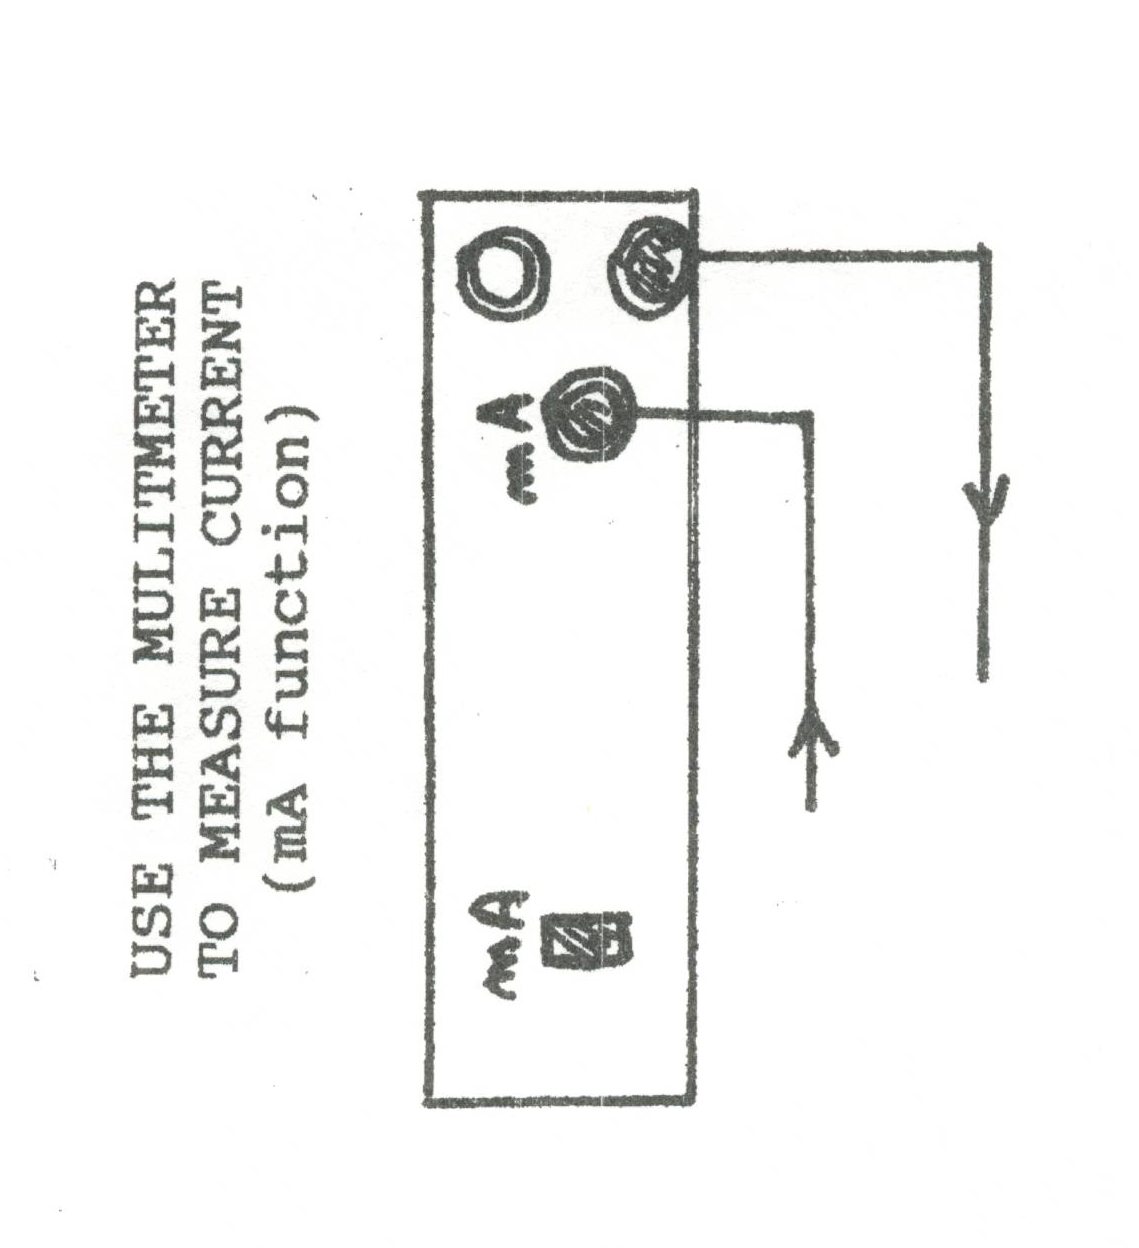
\includegraphics[scale=0.4]{5bgraf/fig_10a}\label{f:fig10a}}
	\mfcaption{Circuit board arrangement for Kirchoff's rules}\label{f:circboard}
\end{center}


\paragraph {Conclusions:}  What general conclusions can you make concerning the internal resistance of batteries and the application of Kirchhoff's rules?

%--begin comment---------------------------------------------------------
\begin{comment}
\begin{enumerate}
	\item Determining the Internal Resistance of a Battery
	\begin{enumerate}
		\item Set up the following circuit.  Use a precision resistor for $R$ and estimate the current that will flow so that you can choose an appropriate scale for the ammeter.

\begin{figure}
	\centering
	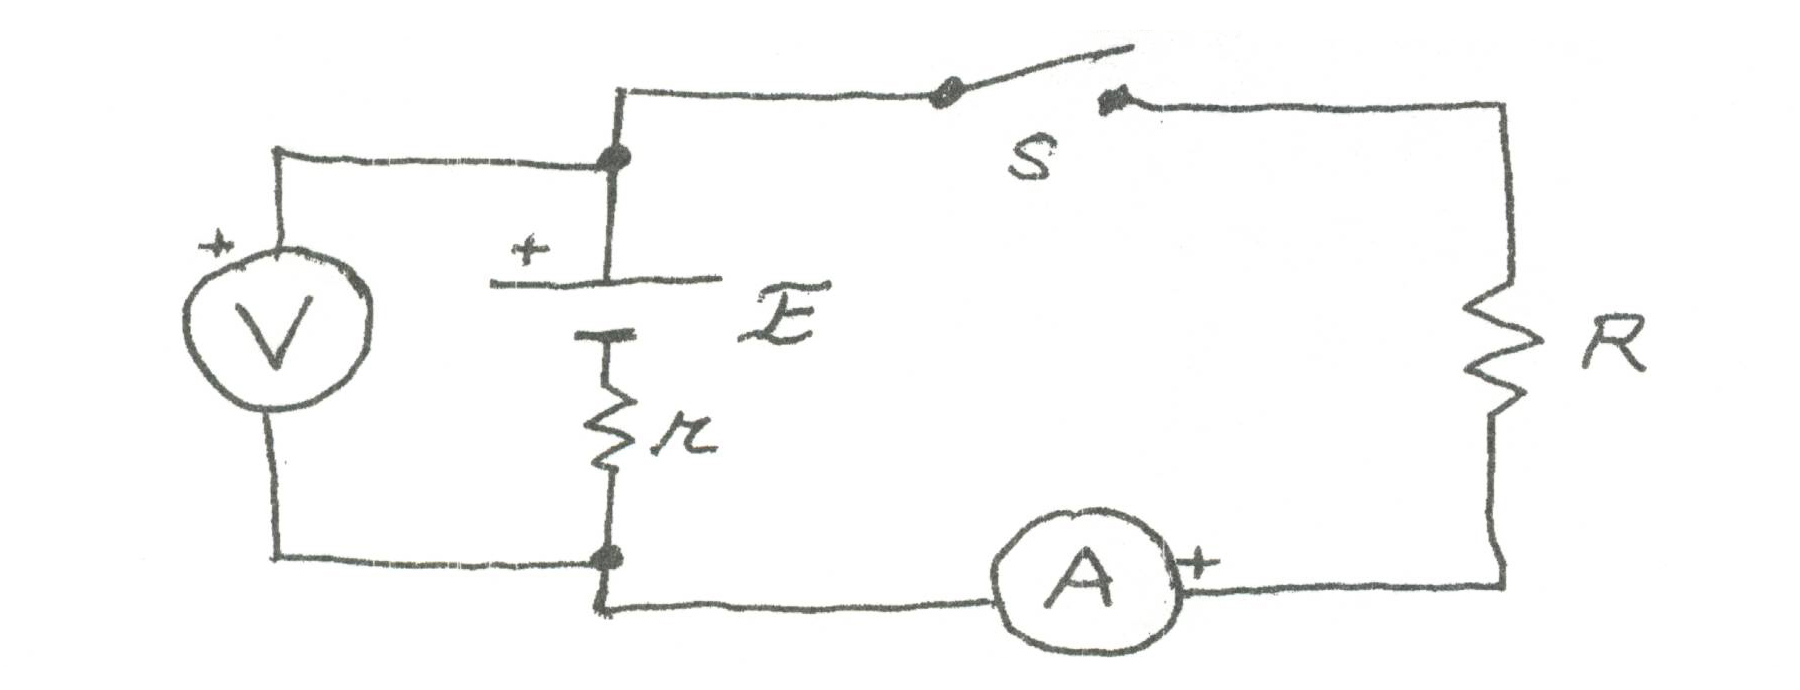
\includegraphics[scale=0.8]{5bgraf/fig_8}
	\caption{Setup to measure internal resistance of a battery}
	\label{f:fig8}
\end{figure}

		\item Measure and record the current and terminal voltage as accurately as possible.
		\item Replace the precision resistor with one having a different resistance and repeat the measurements of current and terminal voltage.
		\item Calculate the internal resistance $r$ of the battery for each measurement taking the emf to be $E = 1.54 V$.  Are your values consistent?  If not, it may be that the internal resistance actually varies with load.  Discuss these results and your observations regarding the internal resistance of your battery in your lab report.
	\end{enumerate}
	\item Kirchhoff's rules
	
	\begin{enumerate}
		\item Measure the emfs of both of your batteries.  Assuming the voltmeter has high resistance, the emf, $E$ is the voltage you measure with the battery alone connected to the voltmeter.
		\item Assemble the circuit shown in fig. \ref{f:fig_9}.  (See fig. \ref{f:fig10b} for a pictorial representation of the circuit.)

\begin{figure}
	\centering
	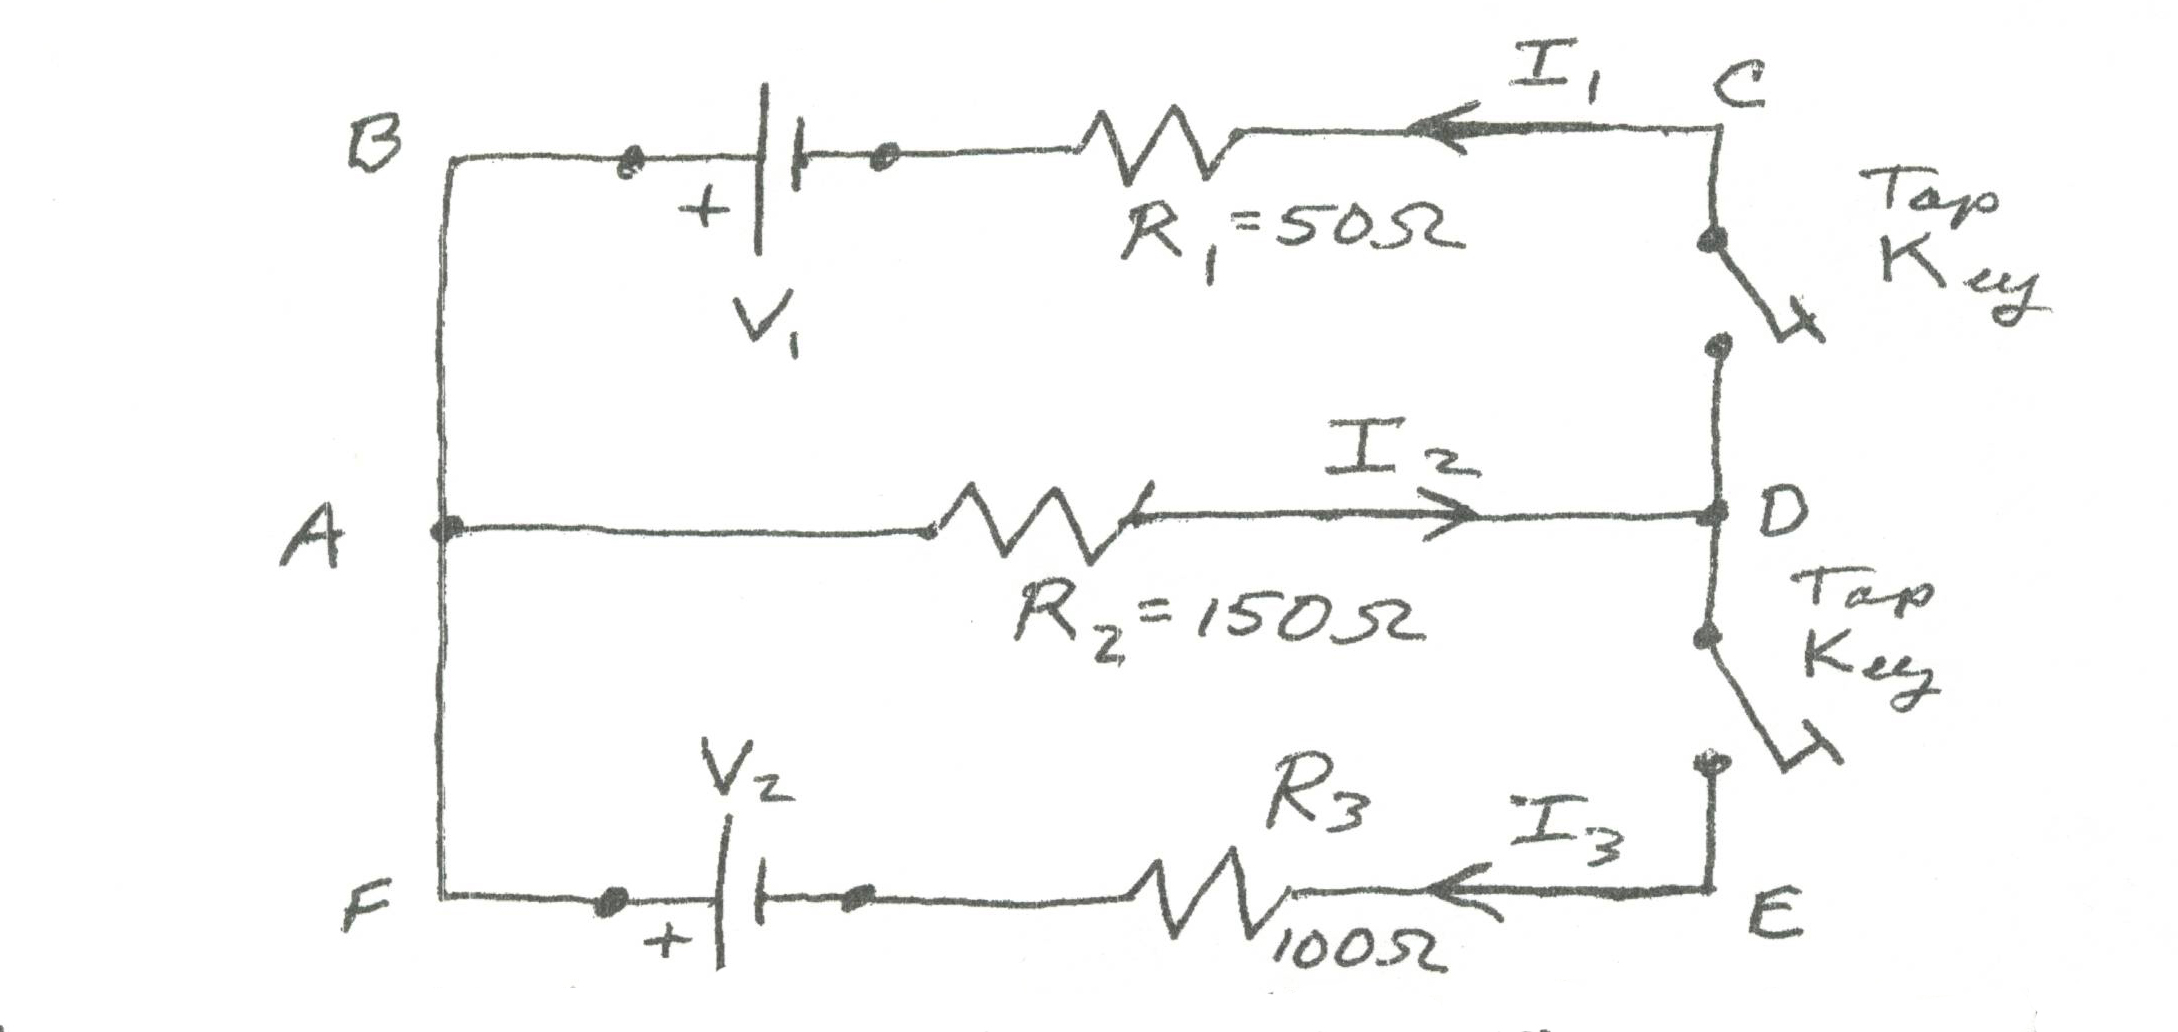
\includegraphics[scale=0.8]{5bgraf/fig_9}
	\caption{Multiloop circuit with 3 unknown currents}
	\label{f:fig9}
\end{figure}

		\item Measure the terminal voltages of your batteries with both tap keys held down.
		\item Using the diagram on the next page as a guide, measure the currents $I_1$, $I_2$, and $I_3$, by removing the appropriate wire and running the current that would flow through that wire through the ammeter.
		\item Apply Kirchhoff's junction rule to junction $A$ and Kirchhoff's loop rule to the top and bottom loop.  Enter the values of the currents, resistances, and voltages for this circuit into each equation.  Are the rules verified by your values? Discuss your results.
		\item Solve the three equations obtained from the application of Kirchhoff's rules for the currents $I_1$, $I_2$, and $I_3$, treating them as unknowns.  (Your instructor will provide some guidance in how to solve three equations for three unknowns.)  Then calculate the currents using the known values of the resistances and voltages.  Compare the calculated values of the currents to the measured values and discuss how well they agree.
	\end{enumerate}
\end{enumerate}
\end{comment}
%--end comment----------------------------------------------------------


%\begin{figure}
%	\centering
%	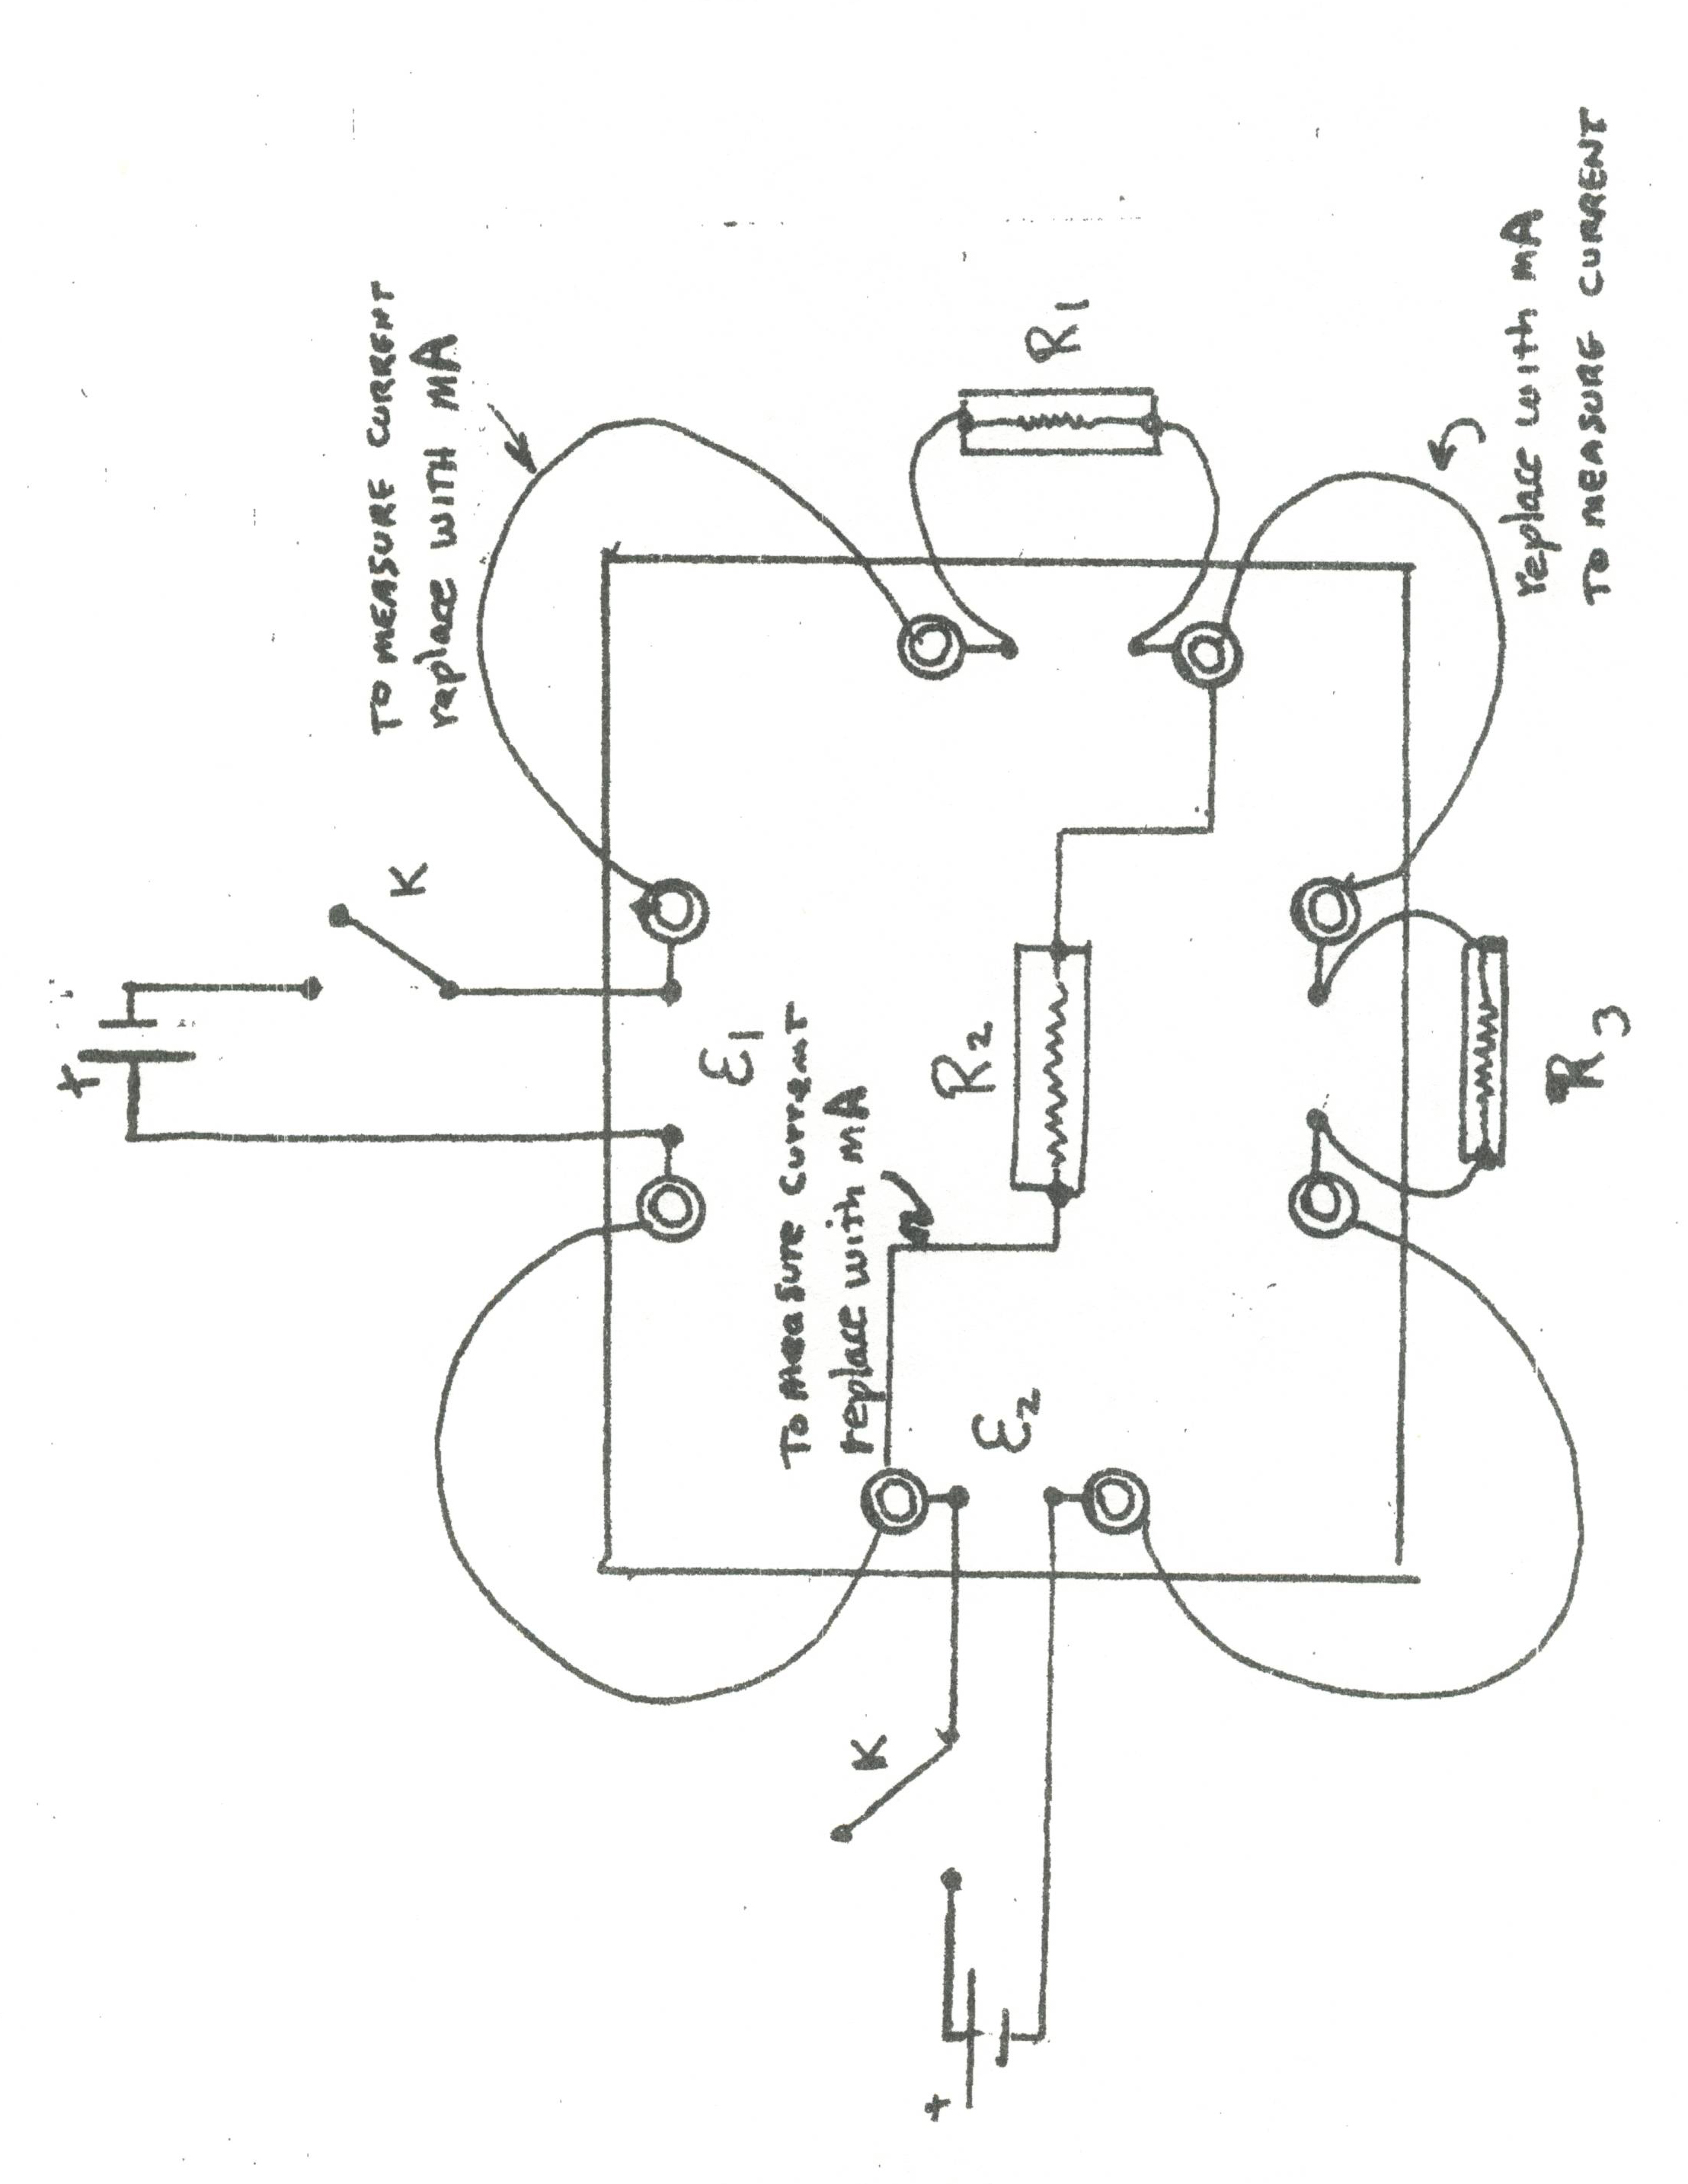
\includegraphics[scale=0.8]{5bgraf/fig_10b}
%	\caption{Circuit board arrangement for Kirchoff's rules}
%	\label{f:fig10b}
%\end{figure}

%\begin{figure}
%	\centering
%	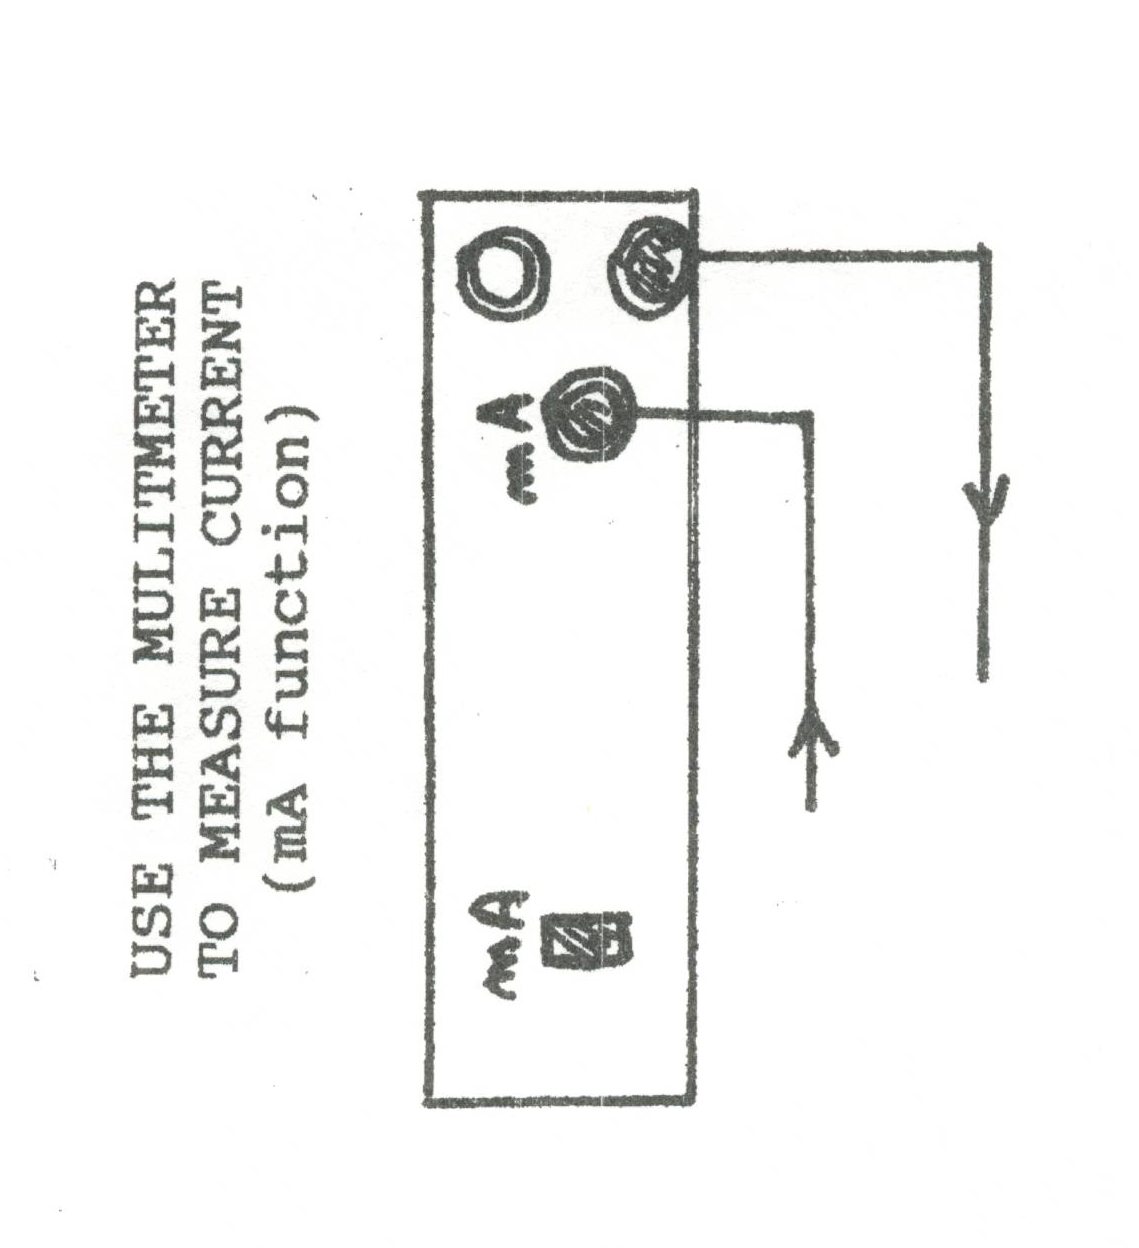
\includegraphics[scale=0.4]{5bgraf/fig_10a}
%	\caption{Multimeter for current measurement}
%	\label{f:fig10a}
%\end{figure}

%--------------------------------------------------------------------------
\endinput
%--------------------------------------------------------------------------
				%--lab 05-------------------------------------

%--------------------------------------------------------------------------
% !TEX root = 5Blman.tex
% induction.tex
% 2013.01.07 changed to 2col format
%--------------------------------------------------------------------------
\chapter{Electromagnetic Induction}

\begin{multicols}{2}
%---------------------------------------------------------------------
\section{Purpose}
The purpose of this laboratory exercise is to explore the phenomenon of electromagnetic induction.  Electromagnetic induction is the creation of an emf using magnetic fields.  It is the basis of most electric generators as well as being responsible for a number of other effects.  The connections between electric and magnetic forces shown by electromagnetic induction is also evidence of the underlying unity of physical laws.

%---------------------------------------------------------------------
\section{Preparation}
Reread the sections in your text on electromagnetic induction before coming to lab. Pay special attention to the concepts of magnetic flux, Faraday's law of induction, and Lenz's law.  You should also review the \textsf{right hand rule for forces} of magnetic fields produced by currents --- in wires and by loops of wire.  You should be able to apply the \textsf{right hand rule for forces} to similar situations as shown in \reffig{f:fig11} to perform this lab.


%\begin{figure}[hbt]
%	\centering
%	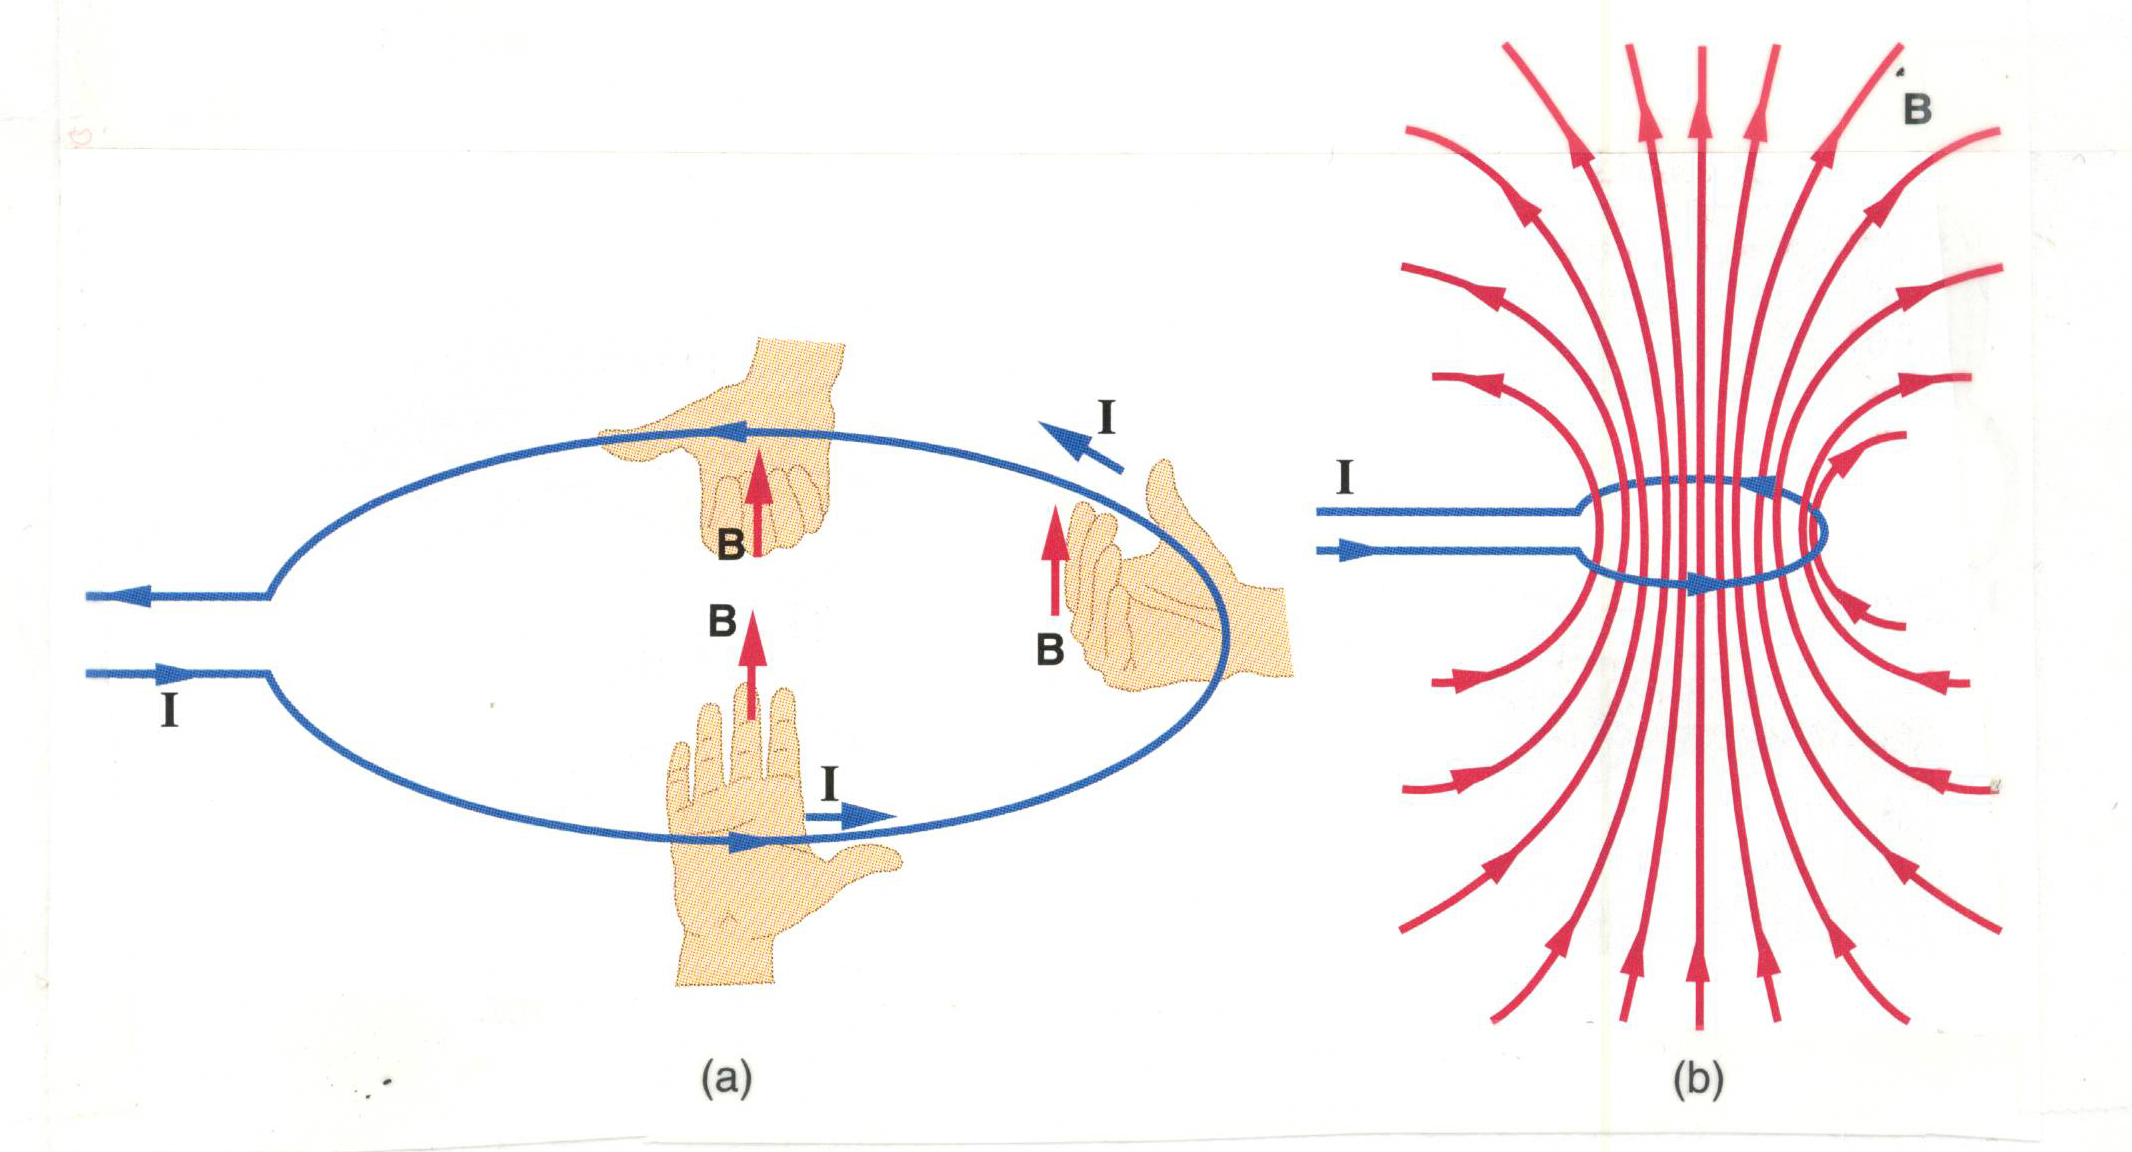
\includegraphics[scale=0.6]{5bgraf/fig_11}
%	\caption{Right hand rule for magnetic fields}
%	\label{f:fig11}
%\end{figure}

\begin{center}
	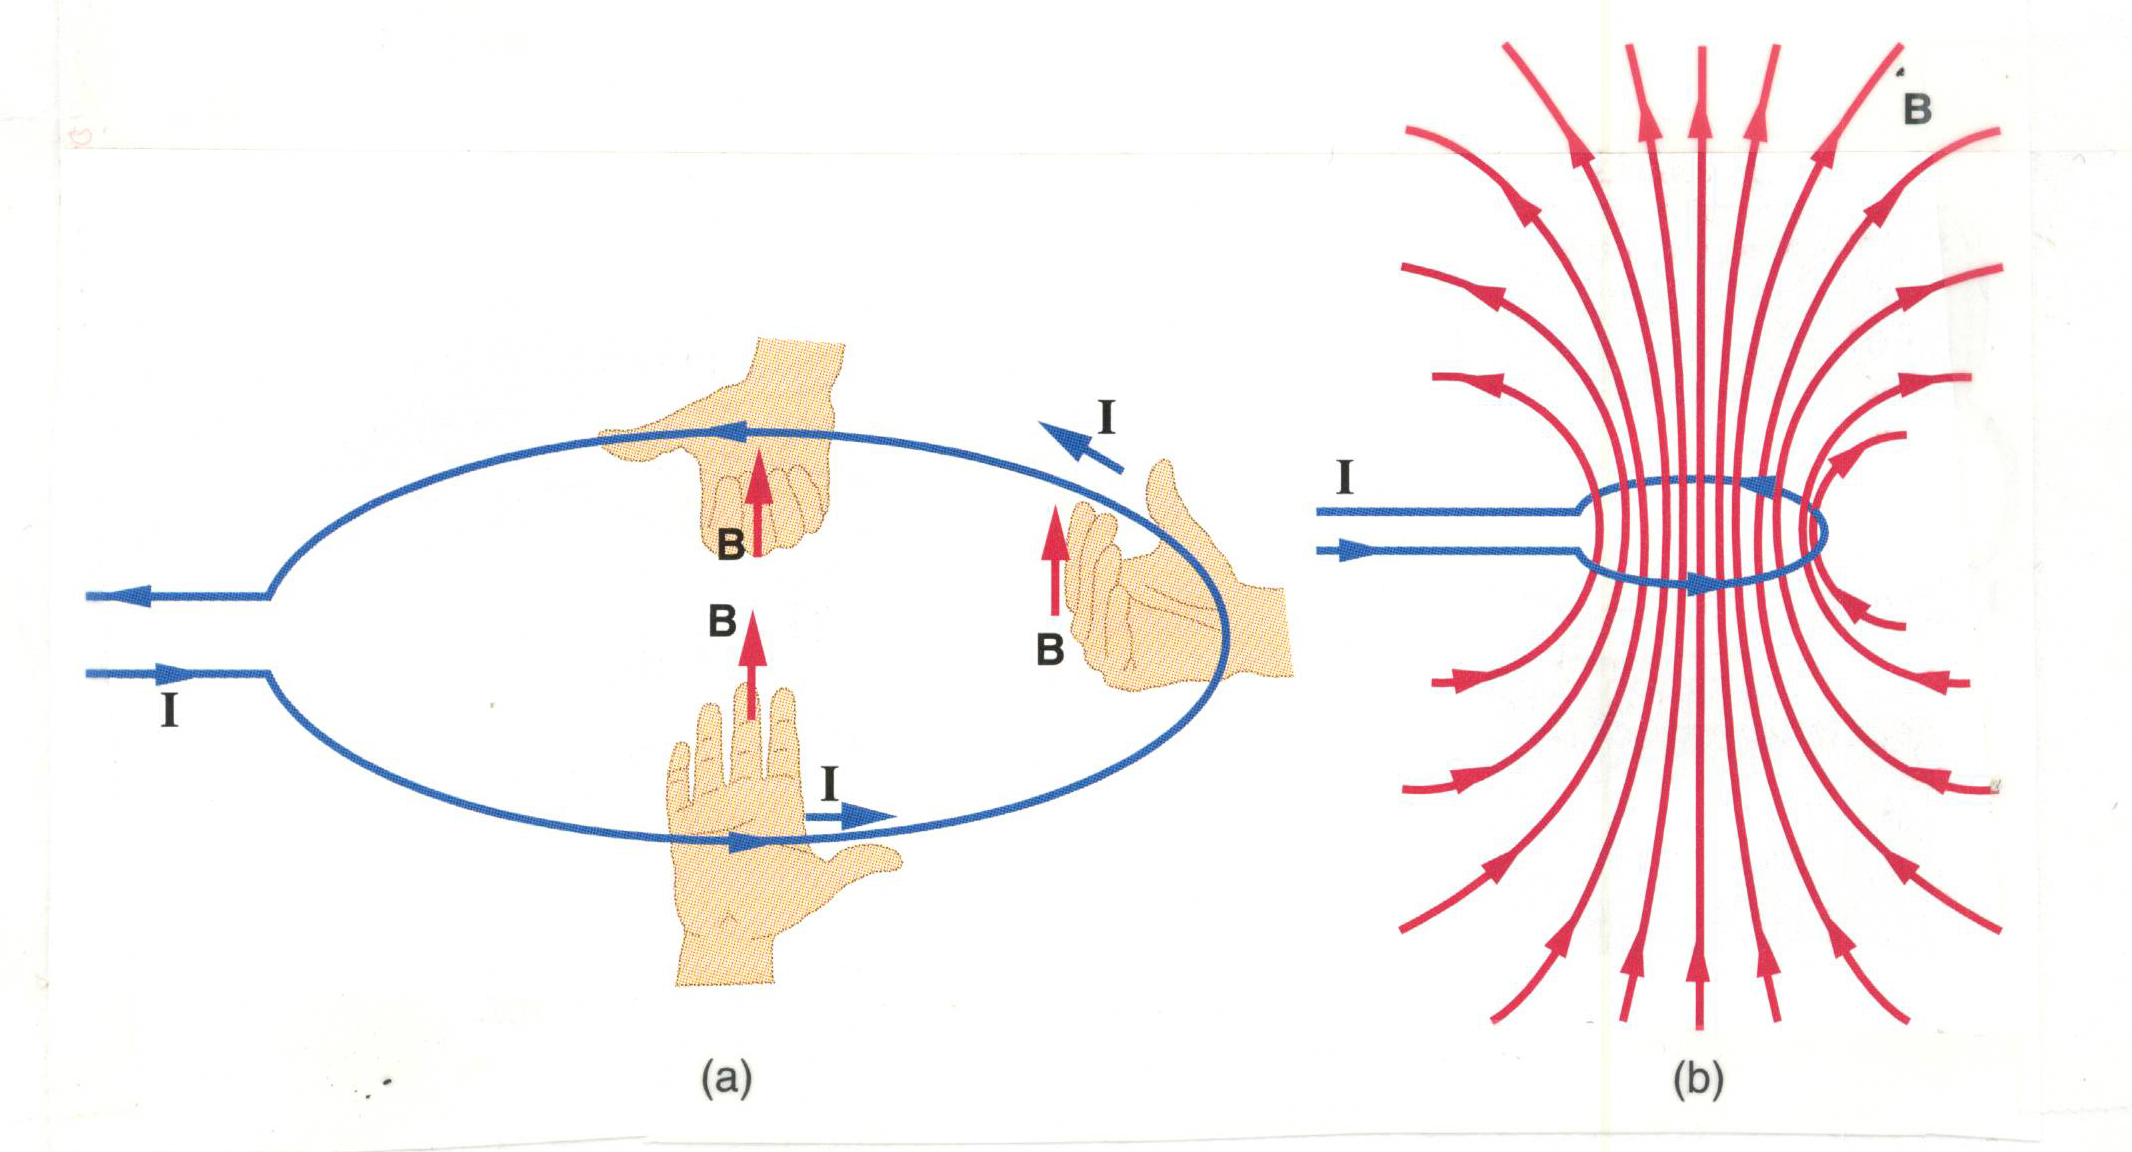
\includegraphics[scale=0.6]{5bgraf/fig_11}
	\mfcaption{Right hand rule for magnetic fields}
	\label{f:fig11}
\end{center}

\paragraph{Short problem}
Suppose the current in coil 1 is increasing in \reffig{f:fig12}.  Explain the direction of the current induced in coil 2 using Faraday's law, Lenz's law, and RHR-2.  You may be asked to turn in your explanation at the beginning of class as a short preparatory quiz.

%\begin{figure}
%	\centering
%	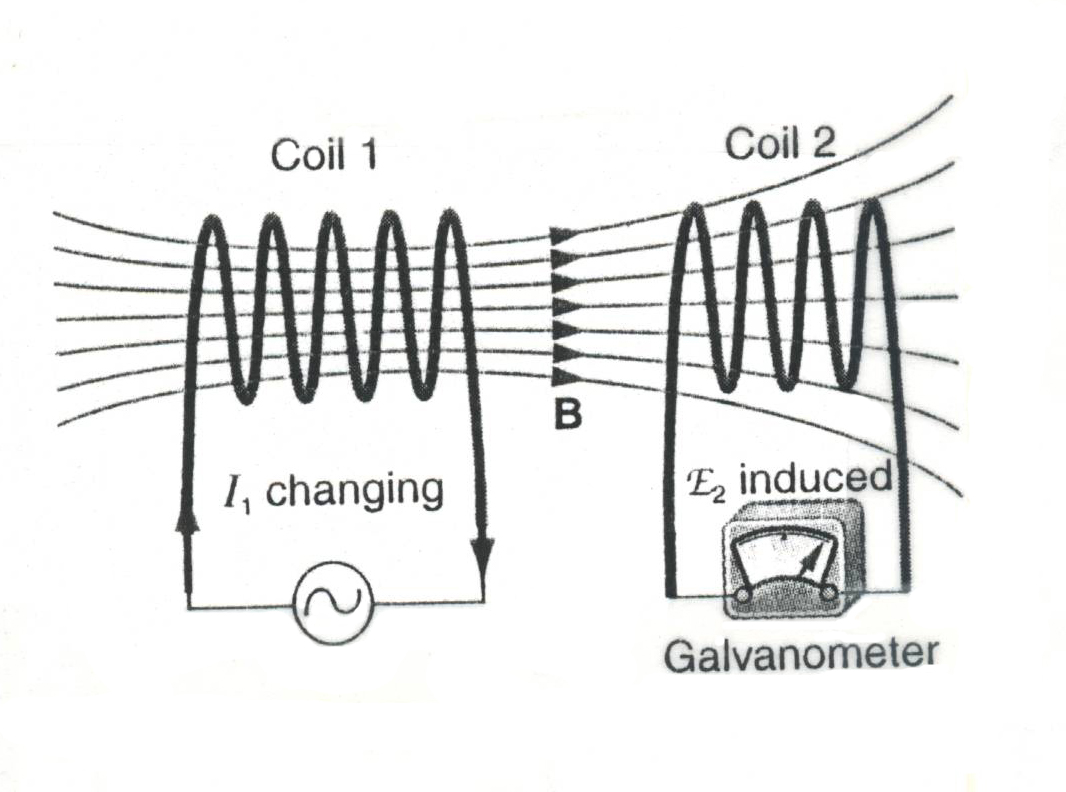
\includegraphics[scale=0.8]{5bgraf/fig_12}
%	\caption{A changing current in one coil induces an EMF in another coil}
%	\label{f:fig12}
%\end{figure}

\begin{center}
	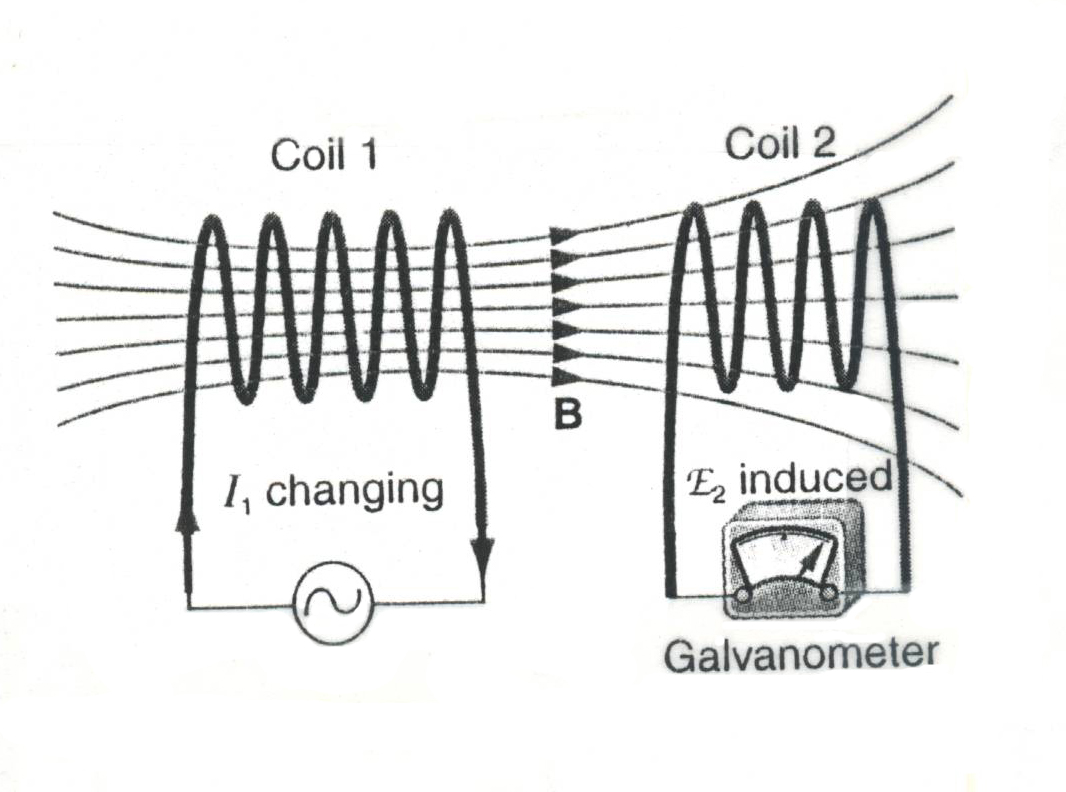
\includegraphics[scale=0.8]{5bgraf/fig_12}
	\mfcaption{A changing current in one coil induces an EMF in another coil}
	\label{f:fig12}
\end{center}

%---------------------------------------------------------------------
\section{Experimental Set-Up}
You will use two coils in a series of activities.  These are shown in \reffig{f:fig13} as one of the configurations you will explore.  The primary coil is the one that you connect to a battery and switch.  The secondary coil is the one you connect to a galvanometer.  Current into the + side of the galvanometer causes a deflection of the meter to the right: this allows you to determine the direction and relative magnitude of any current induced in the secondary.


%\begin{figure}
%	\centering
%	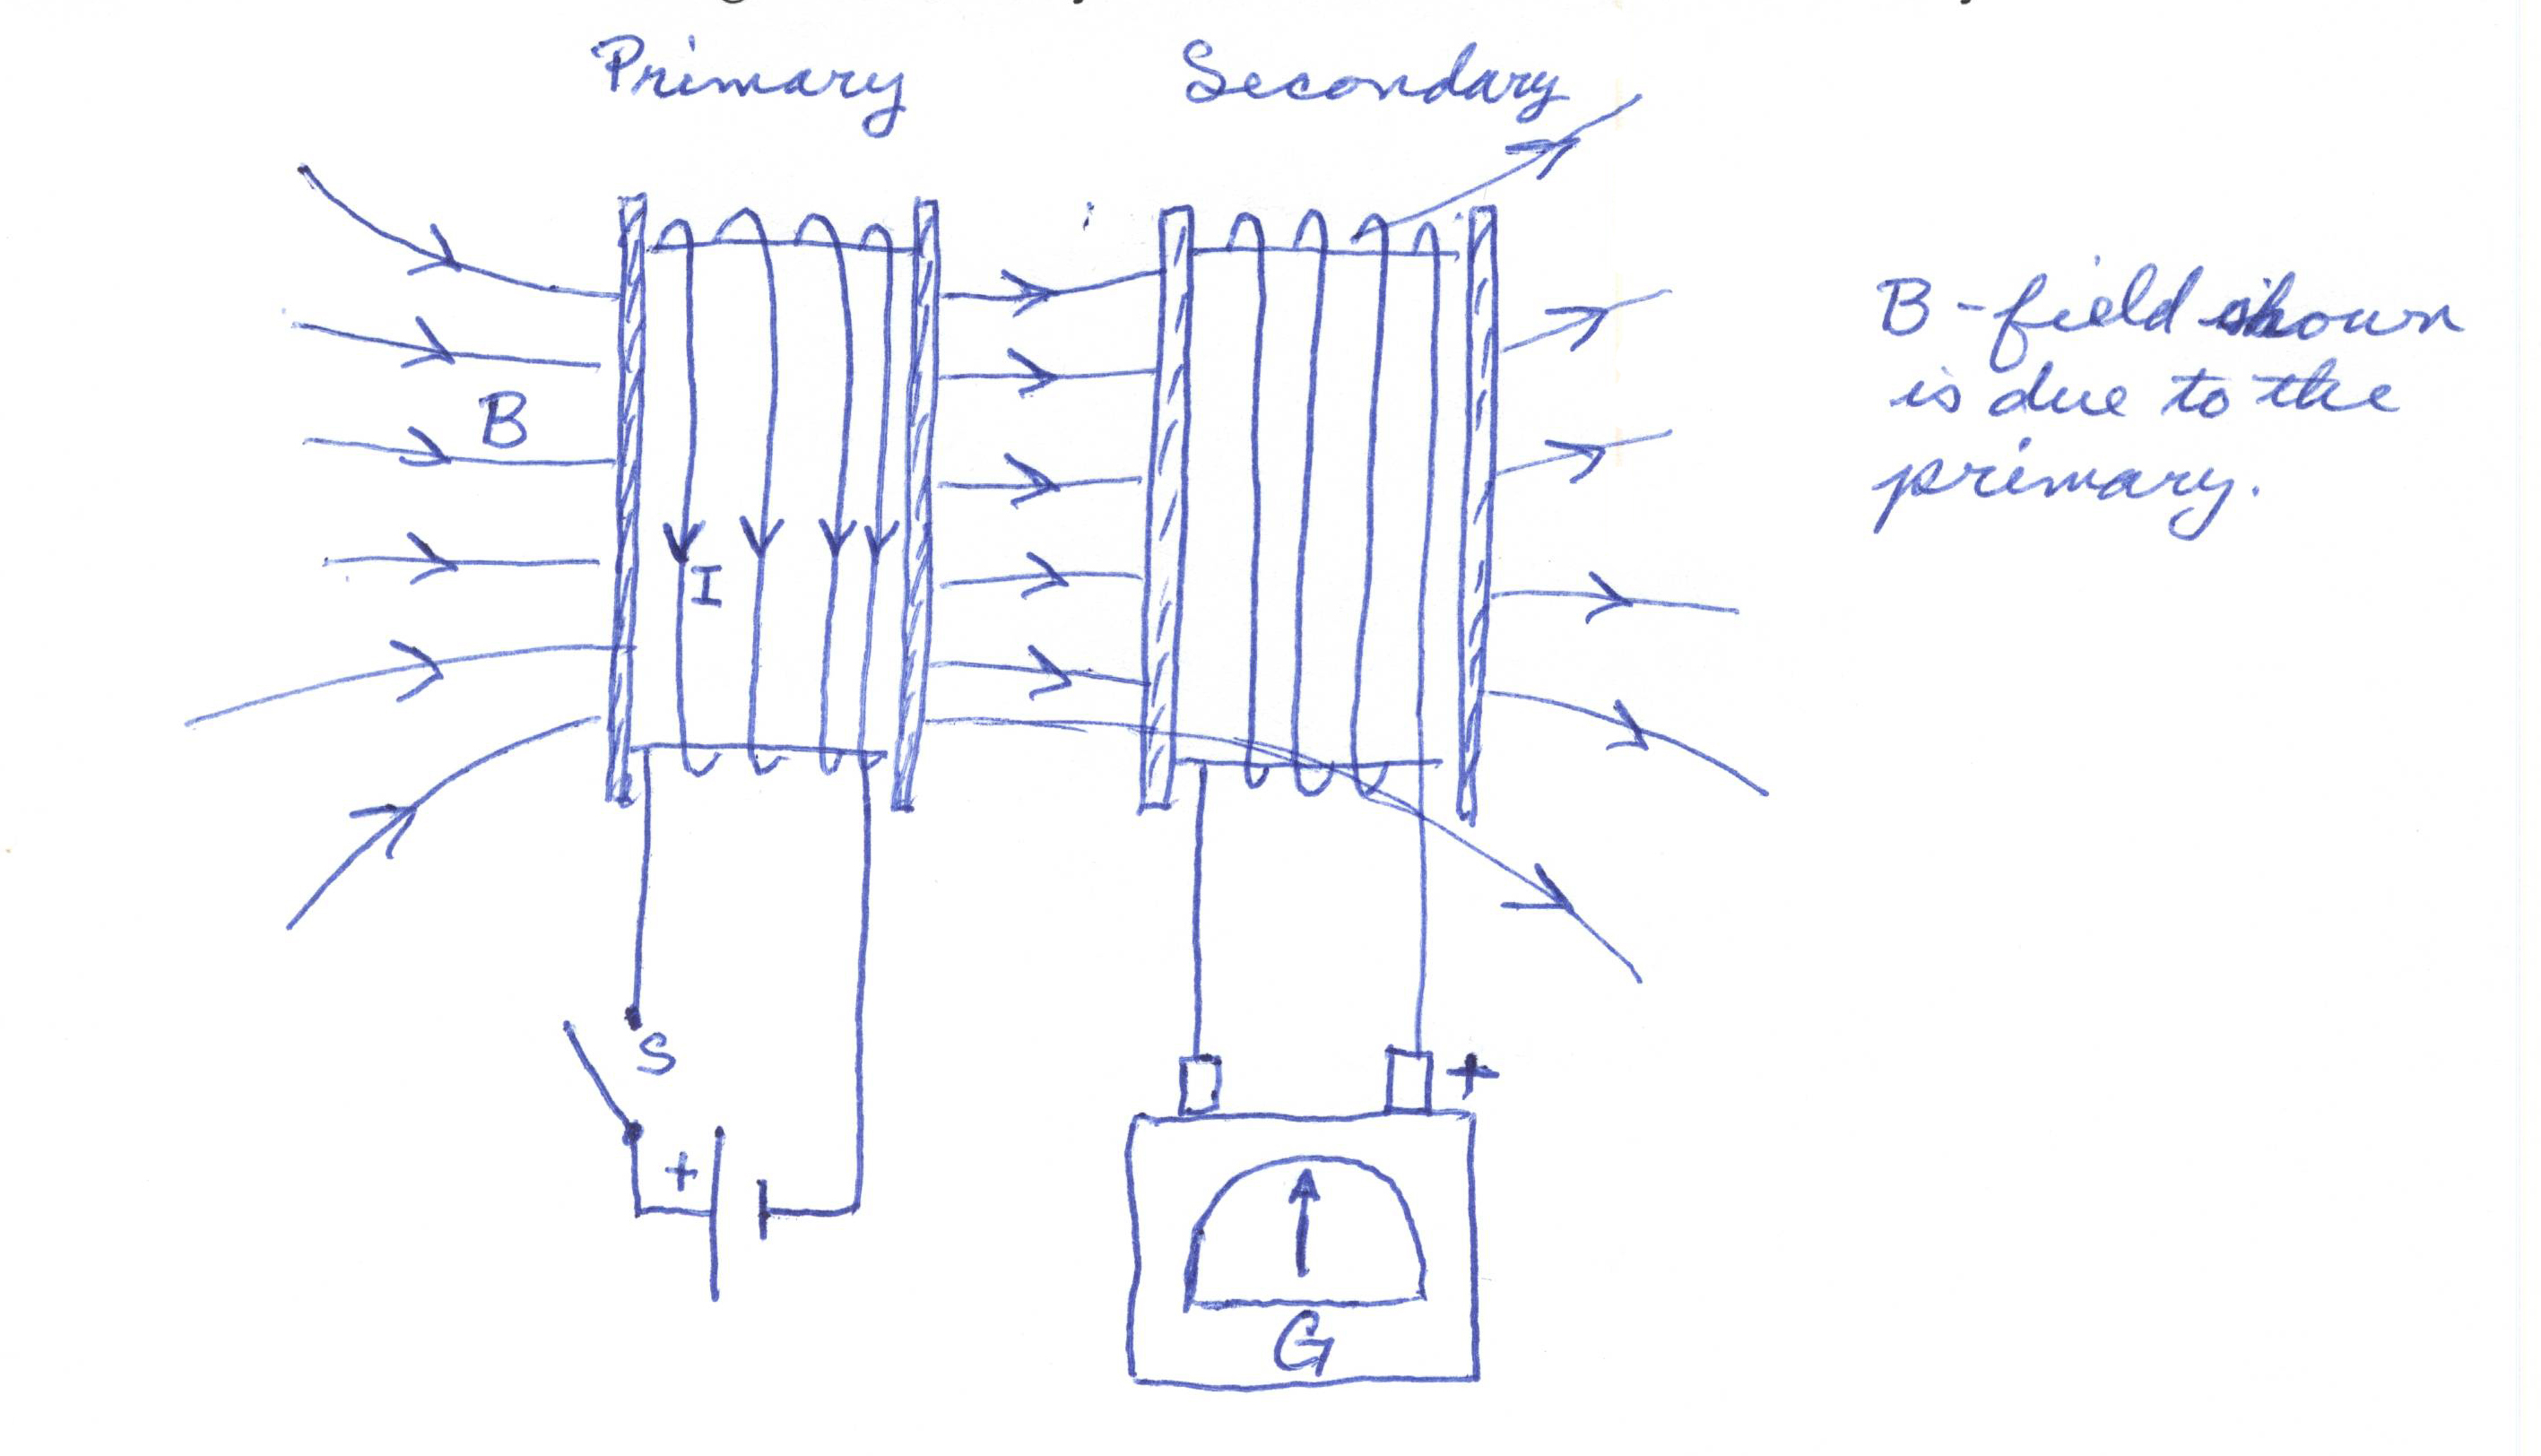
\includegraphics[scale=0.6]{5bgraf/fig_13}
%	\caption{Primary and secondary coils illustrate Lenz's law}
%	\label{f:fig13}
%\end{figure}

\begin{center}
	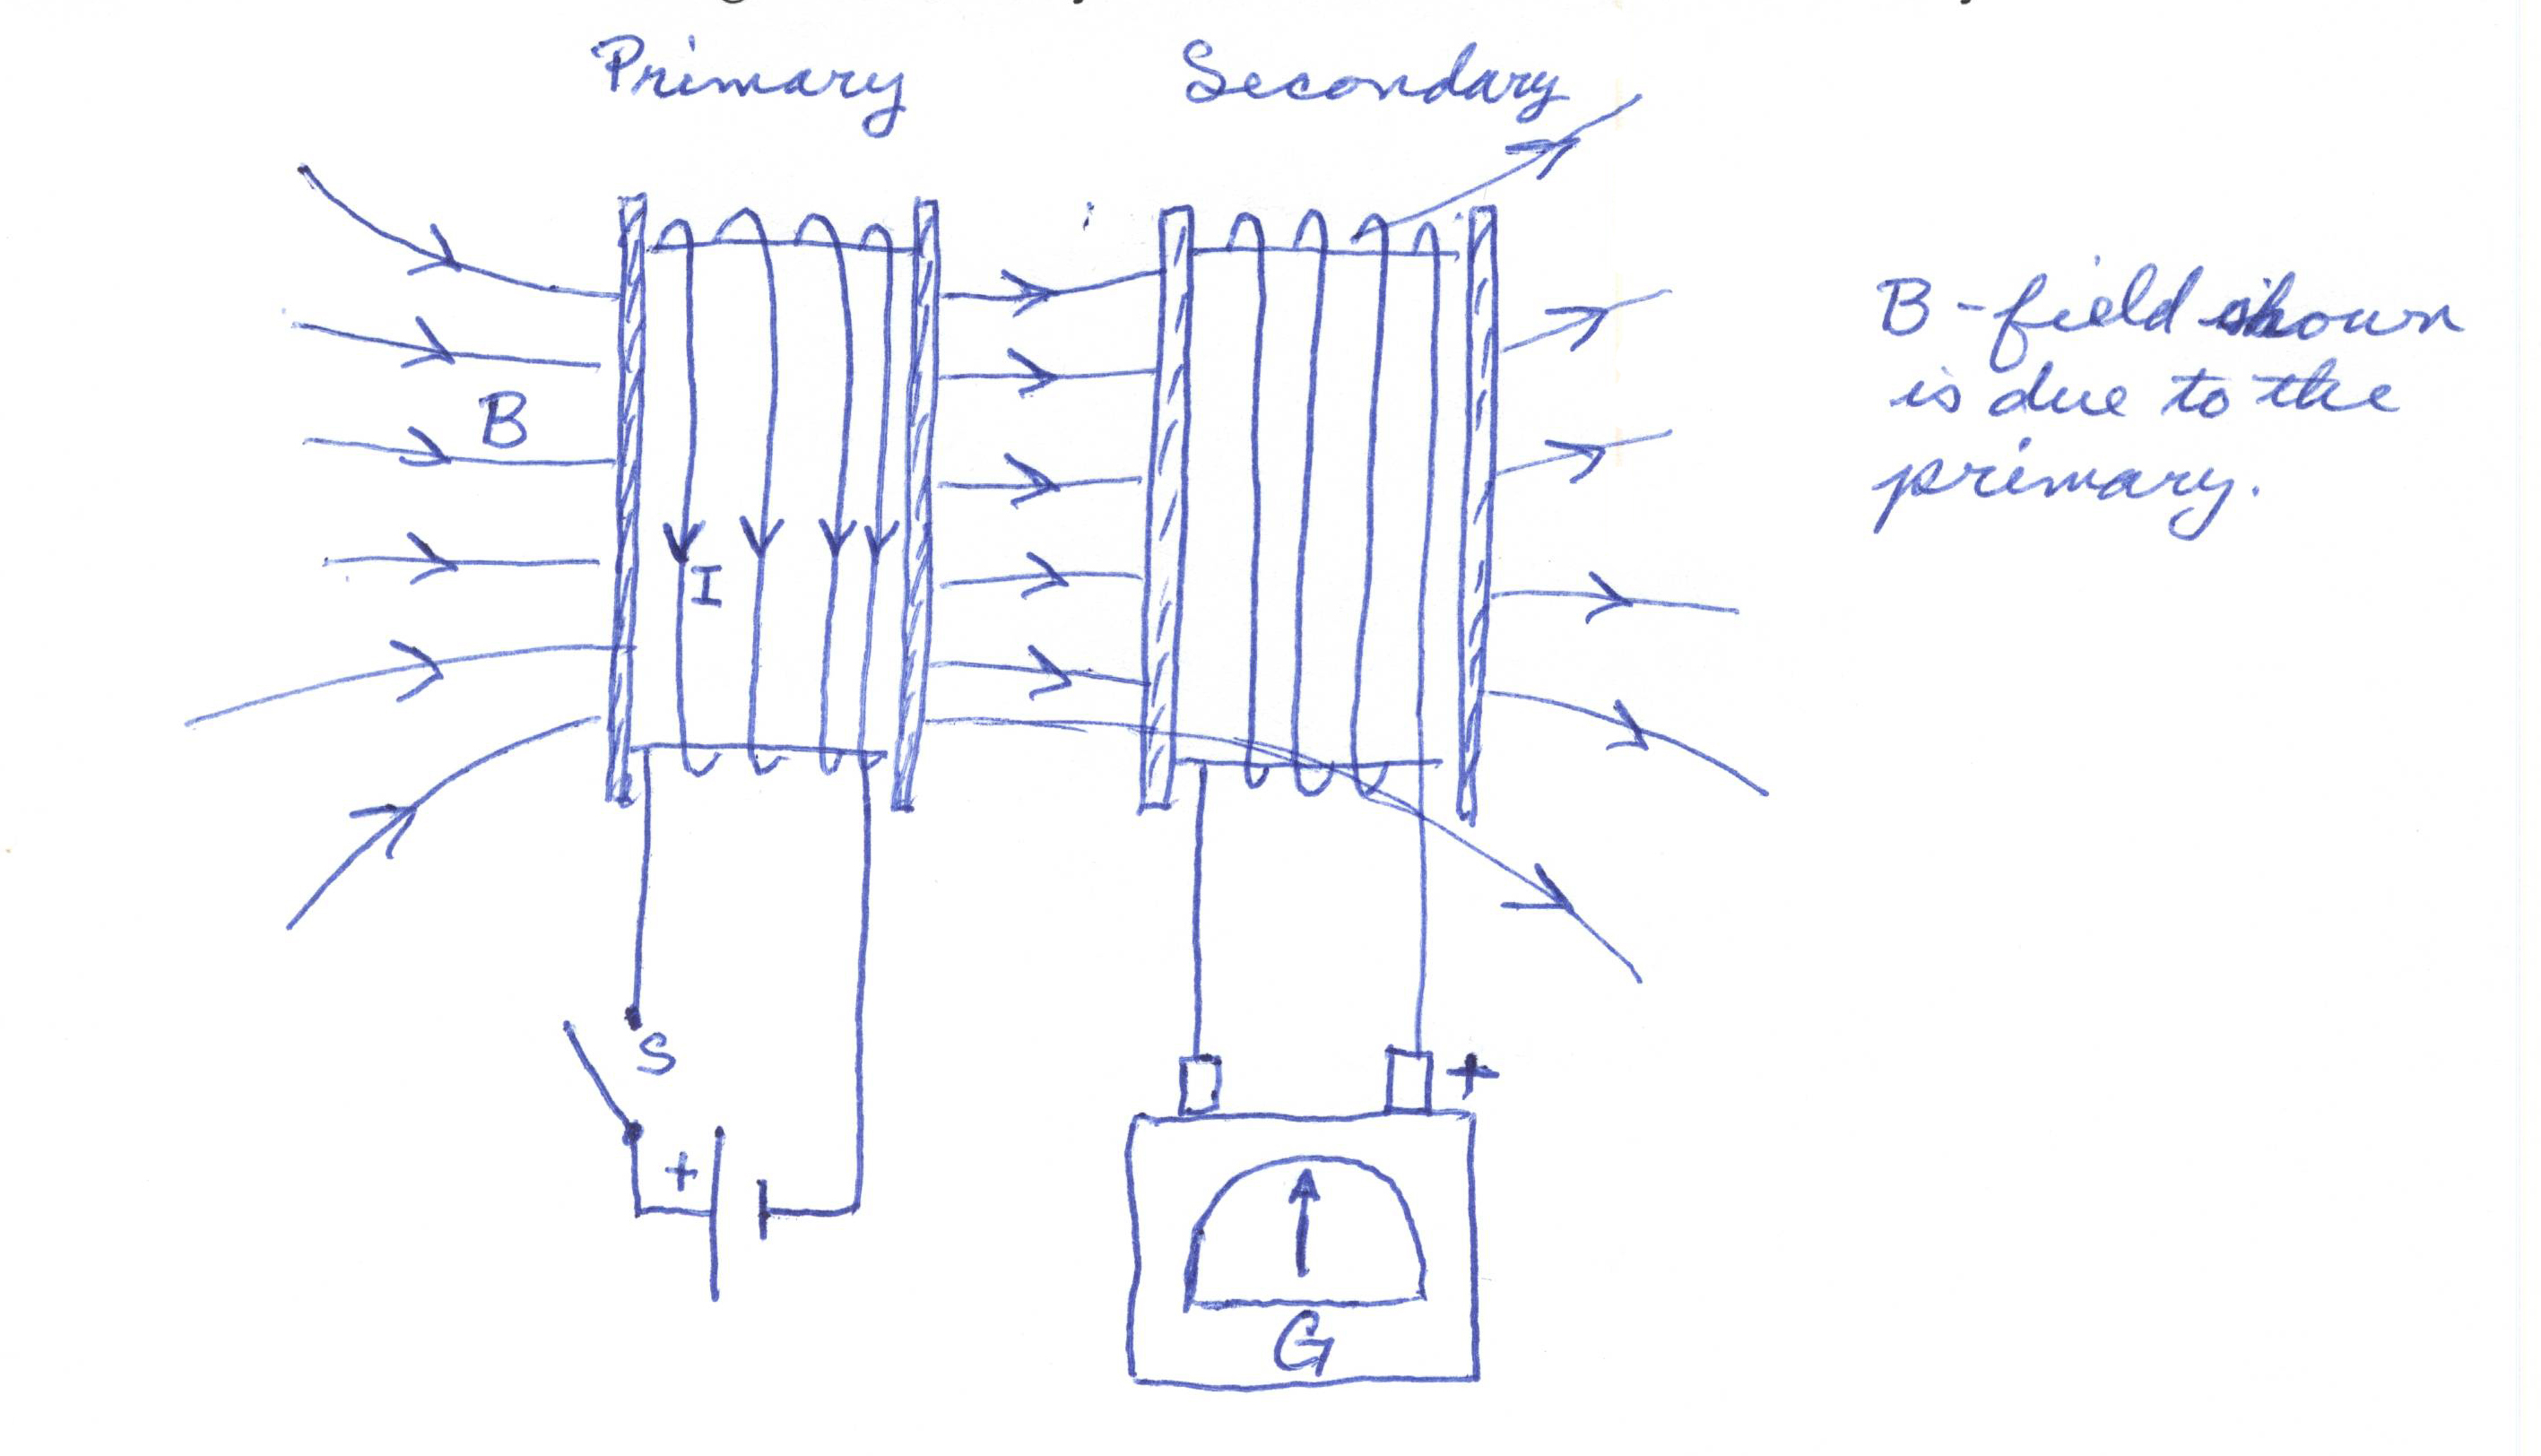
\includegraphics[scale=0.45]{5bgraf/fig_13}
	\mfcaption{Primary and secondary coils illustrate Lenz's law}
	\label{f:fig13}
\end{center}

%---------------------------------------------------------------------
\section{Exploring Magnetic Induction}

\subsection{Activity: Magnetic field and current direction}
% Verification of RHR-2
\begin{enumerate}
	 \item 	Use the primary coil and the small compasses to verify the \textsf{right hand rule for forces} -- that is, verify the relationship of the direction of the magnetic field to the direction of current through the primary coil.
	 \item 	Note that current flows out of the + terminal of the battery and that the magnetic field direction is (by definition) the direction that the north seeking end of a compass points.  You should explore the direction of the field inside and outside of the coil first for current flowing in one direction and again for current flowing in the opposite direction.
	 \item 	Make drawings that indicate the direction of current and magnetic field in both cases.  Explain how the direction of the field is consistent with the \textsf{right hand rule for forces}.
\end{enumerate}

\subsection{Activity: Induced emf by a coil} \label{s:coilind}
% Emf $E$ induced in the secondary coil by the primary coil
	Line up the primary and secondary coils in an arrangement similar to that in \reffig{f:fig13} above with the primary connected to the battery and switch and the secondary connected to the galvanometer.  Be certain that the windings of both coils are in the same direction: that is, both clockwise or both counterclockwise. 
	
	Explain all observations by making drawings and using Faraday's law, Lenz's law, and the \textsf{right hand rule for forces}
\begin{enumerate}
	 \item Open and close the switch.  What direction does the galvanometer deflect?  Does it show a deflection at all times?  
	\item Close the switch and leave it closed.  Move the secondary away from the primary and bring it back.  Note the reaction of the galvanometer and any dependence on how fast the secondary is moved.
	\item Repeat part ($1$), but move the primary instead of the secondary cois.
	\item Use an iron rod to link the primary and secondary coils instead of the wood rod.  Starting with the coils separated by 10 cm, open and close the switch to the primary.  Record the relative magnitude of the deflection of the galvanometer then decrease the separation of the coils to 9 cm, then 8 cm, and so on.  Make a graph of the galvanometer deflection versus distance between the coils. 
\end{enumerate}

\subsection{Activity: Induced emf by a magnet}
% Emf $E$ induced in the secondary coil by a bar magnet
\begin{enumerate}
	 \item First verify with small compasses that the bar magnet has its poles correctly labeled.
	\item  Remove the primary coil and keep the secondary coil connected to the galvanometer.  Thrust the north pole of the bar magnet into the core of the secondary coil.  Then pull it out.  Repeat with the south pole of the bar magnet.  Examine the effect of the speed of the motion.  
	\item Explain all observations by making drawings and using Faraday's law, Lenz's law, and the \textsf{right hand rule for forces}.  Also verify that the observations are consistent with those obtained in activity \ref{s:coilind}. 
\end{enumerate}

%---------------------------------------------------------------------
\section{Conclusions}
 What aspects of Faraday's law, Lenz's law, and the \textsf{right hand rule for forces} have you verified in today's laboratory exercise?
 
% \clearpage
%\newpage
%\includegraphics*[width=\textwidth,trim=120 80 80 120,clip]{5bgraf/pslabgrid} 

\end{multicols}
%--------------------------------------------------------------------------
\endinput
%--------------------------------------------------------------------------
		%--lab 06-------------------------------------

%--------------------------------------------------------------------------
% !TEX root = 5Blman.tex
% emrad.tex
%--------------------------------------------------------------------------
\chapter{Electromagnetic Radiation}

\section{Purpose}
  The purpose of this laboratory exercise is to explore both the wave and photon nature of electromagnetic radiation.  In the process you will manipulate and observe several distinct types of electromagnetic radiation ranging from microwaves to x rays, thereby gaining a hands-on familiarity with these entities.

\section{Preparation}
  Read the sections in your text and become familiar with the electromagnetic spectrum before coming to lab.  Note the definitions of the various types of electromagnetic waves.  Pay special attention to the effects of these waves, the manner in which they are created, and how they may be detected.

\paragraph{Short quiz}
  Be prepared to take a short quiz for which you need to be familiar with the major categories of electromagnetic waves and their properties.
\section{General Information}

Your instructor will explain the operation of the numerous pieces of apparatus in the room.  There is only one station for each activity so you will circulate about the room to perform this lab.  You may perform the activities in any order.
Your instructor will also summarize the wave and photon characteristics of electromagnetic radiation.

\section{Exploring EM radiation}
Perform each of the following activities.  Be certain to keep good records of your observations and to answer the specific questions posed.  Note anything that you observe in addition to what is mentioned in this write up.  Such observations may be at least as important as those you are asked to make.

\subsection{Microwaves}
Microwaves are the highest-frequency electromagnetic waves that can be produced by currents in circuits.  They generally have a frequency that is the same as the oscillation frequency of the circuit.

\begin{enumerate}
	\item Sketch the microwave apparatus, labeling the major components.  Note that the only evidence for the microwaves is given by the meter connected to a detection device.
	\item Can you feel the microwaves?  Why don't they cook you like a microwave oven would?
	\item Explore the microwaves for evidence that the wavelength is on the order of the size of the wave guides that carry the microwaves (about 4 cm).  Describe your method and observations.  Calculate the frequency of the microwaves assuming they have a 4.00 cm wavelength. \par
	Alternatively, use the data in Table \ref{t:microwavesignal} to determine the microwave wavelength and frequency.
	\item Explore the microwaves for evidence of polarization.  Describe your method and observations.  Is polarization a characteristic of waves?  Explain briefly.
\end{enumerate}
	
\subsection{Infrared (IR)}
Infrared radiation is usually produced by thermal motion and the vibration and rotation of atoms and molecules.  Its frequencies overlap with the upper end of the microwave range and extend to the lower end of the visible range hence the name infrared or ``below red.''
\begin{enumerate}
	\item Can you see infrared radiation with your eyes?  How do you detect it in this exercise?  Your skin absorbs about 98\% of the infrared radiation that falls on it.  What "color" is your skin in the infrared?
	\item Manipulate the reflectors to determine whether infrared radiation and visible light follow the same laws of reflection.  Perform a similar experiment with the large lens.  Do your results support the contention that infrared and visible light behave similarly?
\end{enumerate}
	
\subsection{Visible Light} 
Visible light is defined to be the part of the electromagnetic spectrum to which the eye normally responds, producing nerve signals.  Visible light can be produced by a wide variety of processes.
\begin{enumerate}
	\item Visible Laser Light
	The name "LASER" is an acronym for Light Amplification by Stimulated Emission of Radiation.  Lasers emit electromagnetic waves that have a very pure frequency and wavelength and which are coherent (all the waves are in phase).  Our lasers emit narrow beams of light and are not dangerous to your vision, but should be treated with caution (like an unloaded gun) since some lasers can easily blind you if the beam enters the eye directly.
	\begin{enumerate}
		\item Pass the laser light through a narrow slit and describe what you observe.  How are your observations consistent with the wave nature of electromagnetic radiation?
		\item Observe the hologram image.  How can you tell that it is a true three-dimensional image?
		\item List several applications of lasers.  Explain how each application is related to the pure frequency and coherent nature of laser output.
	\end{enumerate}
	
	\item Polarization of Visible Light
	\begin{enumerate}
		\item Devise an experiment that demonstrates the polarization of visible light. Two methods are effective and should be explored. The first is the passage of light through certain materials and the second is the reflection of light.
		\item Describe a specific use of a polarizing material.
	\end{enumerate}
	
	\item Visible Spectra	
		Use the diffraction gratings to observe the spectra of the light sources in the large black box.
	\begin{enumerate}	
		\item Sketch the spectrum of each of the five light sources.
		\item What characteristic (if any) of each spectrum is "quantized?"  By quantized we mean that only certain values are observed.
		\item Why does each gas have a different spectrum?
		\item Briefly explain why the filament's spectrum is not quantized (continuous rather than discrete bands of color).
	\end{enumerate}
\end{enumerate}

\subsection {Photoelectric Effect}	
The photoelectric effect is the only observation in today's laboratory exercise that cannot be explained by the wave nature of electromagnetic radiation alone.  It can be explained by the existence of photons (your instructor should discuss the nature of photons or particles of light).
\begin{enumerate}
	\item Describe the operation of the photoelectric apparatus.
	\item Devise an experiment with red and blue filters that implies the photon energy of blue light is greater than the photon energy of red light.
	\item Pick some feature of the photoelectric effect that cannot be explained by waves alone and elaborate on how the wave picture is insufficient to describe this feature.
\end{enumerate}

	
\subsection {Ultraviolet Radiation (UV)}
\begin{enumerate}
	\item Ultraviolet radiation has higher frequencies and hence higher photon energies than visible light.  Many UV characteristics can be explained by the higher photon energy.  One example is the damage done to biological cells by UV.
	\item Fluorescence
	\begin{enumerate}
		\item Observe fluorescence with the black light and the mineral samples provided.
		\item Explain the process of fluorescence in terms of photon energies and atomic excitations and de-excitations.
	\end{enumerate}
	\item A weak source of UV is one with low intensity (a relatively small number of photons emitted per second).  Even weak sources of UV can be good sterilizers and pose a hazard to skin and other living tissue.  Explain why in terms of photon energy.
\end{enumerate}
	
\subsection {X-rays}
X-rays are produced when energetic electrons strike a material.  Inner shell electrons are ejected from some atoms when the incoming electrons strike them.  When another electron fills the hole left, an x-ray is produced.  Cathode ray tubes (such as those in televisions and computer monitors) have energetic electrons that cause a screen to glow.  X-rays are also produced and must be shielded to protect the observer.  Our cathode ray tube is not shielded so you can observe the x-rays it produces.  The intensity of the x-rays is too small to be harmful.
\begin{enumerate}
	\item Describe how you observe the x rays produced by the cathode ray tube.  Does their detection imply the existence of photons?  Explain.
	\item Where do the x-rays seem to originate?
	\item Demonstrate that the x-rays can be shielded against.
	\item How do the damaging properties of x-rays relate to their photon energy?
	\item What precautions are used to protect humans from x-rays produced by televisions and x-ray machines?  Note that all protection involves various combinations of shielding, distance, and time limitation of exposure.
\end{enumerate}

\section{Conclusions}
  For which types of electromagnetic radiation did you observe wave characteristics?  For which did you observe photon characteristics?\\
\hrule 
\begin{table}[b]
\begin{minipage}{0.4\textwidth} 
\centering
\caption{Microwave Peak Signal} \label{t:microwavesignal}
\begin{tabular}{l l l}\toprule
\# & X(cm) & Signal\\
\midrule
1.	&	2.84 &	max\\
2.	&	3.59 &	min\\
3.	&	4.31	 &	max	\\
4.	&	5.09 &	min\\
5.	&	5.86 &	max\\
6.	&	6.57	 &	min\\
7.	&	7.36 &	max\\
8.	&	8.14 &	min\\
9.	&	8.85 &	max\\
10.	& 	9.55 &	min\\
\bottomrule
\end{tabular}
\end{minipage} \hfill
\begin{minipage}{0.5\textwidth} 
The values shown in Table \ref{t:microwavesignal} display the results from a microwave setup. The displacement values, x, are measured along a straight line between the microwave transmitter and receiver. The signal values represent the locations where the voltage strength reaches a minima or maxima. For example, the value x = 2.84 cm indicates the location where the voltage reading is a maxima whereas the location x = 3.59 cm represents a location where the voltage reading is a minima. From these values you can determine the wavelength.
\end{minipage}
\end{table}

%--------------------------------------------------------------------------
\endinput
%--------------------------------------------------------------------------
			%--lab 07-------------------------------------

%--------------------------------------------------------------------------
% !TEX root = 5Blman.tex
% reflect.tex
%--------------------------------------------------------------------------
\chapter{Reflection and Refraction}

\section{Purpose}
  The purpose of these laboratory exercises is to give you hands-on experience with the two basic laws of geometrical optics the laws of reflection and refraction. This lab continues the study of light, in particular the ray nature of light when light interacts with objects that are much larger than its wavelength.
  
\section{Preparation}
Note the definitions of important concepts in your text.  Pay particular attention to the laws of reflection and refraction.  Be certain you are comfortable with the ray model of light and the manner in which angles are denoted to specify the direction of a light ray.
\paragraph{Short quiz}
  Be prepared to take a short quiz at the beginning of lab related to the concepts associated with this laboratory exercise.
\section{General Information}

\paragraph{Warning}
  Never look directly into a laser beam and do not shine the beam into anyone's eye.  The lasers used in this laboratory are considered to be relatively safe, but should be treated with caution since lasers that are similar in appearance can have intensities great enough to do permanent harm to the eye.  
  
We use lasers in this laboratory exercise because they produce a narrow beam of monochromatic light.  The path of the light can therefore be more accurately determined than with other light sources.  (This underlies many of the applications of lasers.)  The path of light is a straight line until it interacts with some object.  When light encounters an object that is much larger than its wavelength  (as is the case in this laboratory exercise), it behaves like a ray and its direction is changed in accordance with the laws of reflection and refraction.
 
To measure the direction of a ray of light produced by a laser we use the set up shown here schematically.

\begin{figure}
	\centering
	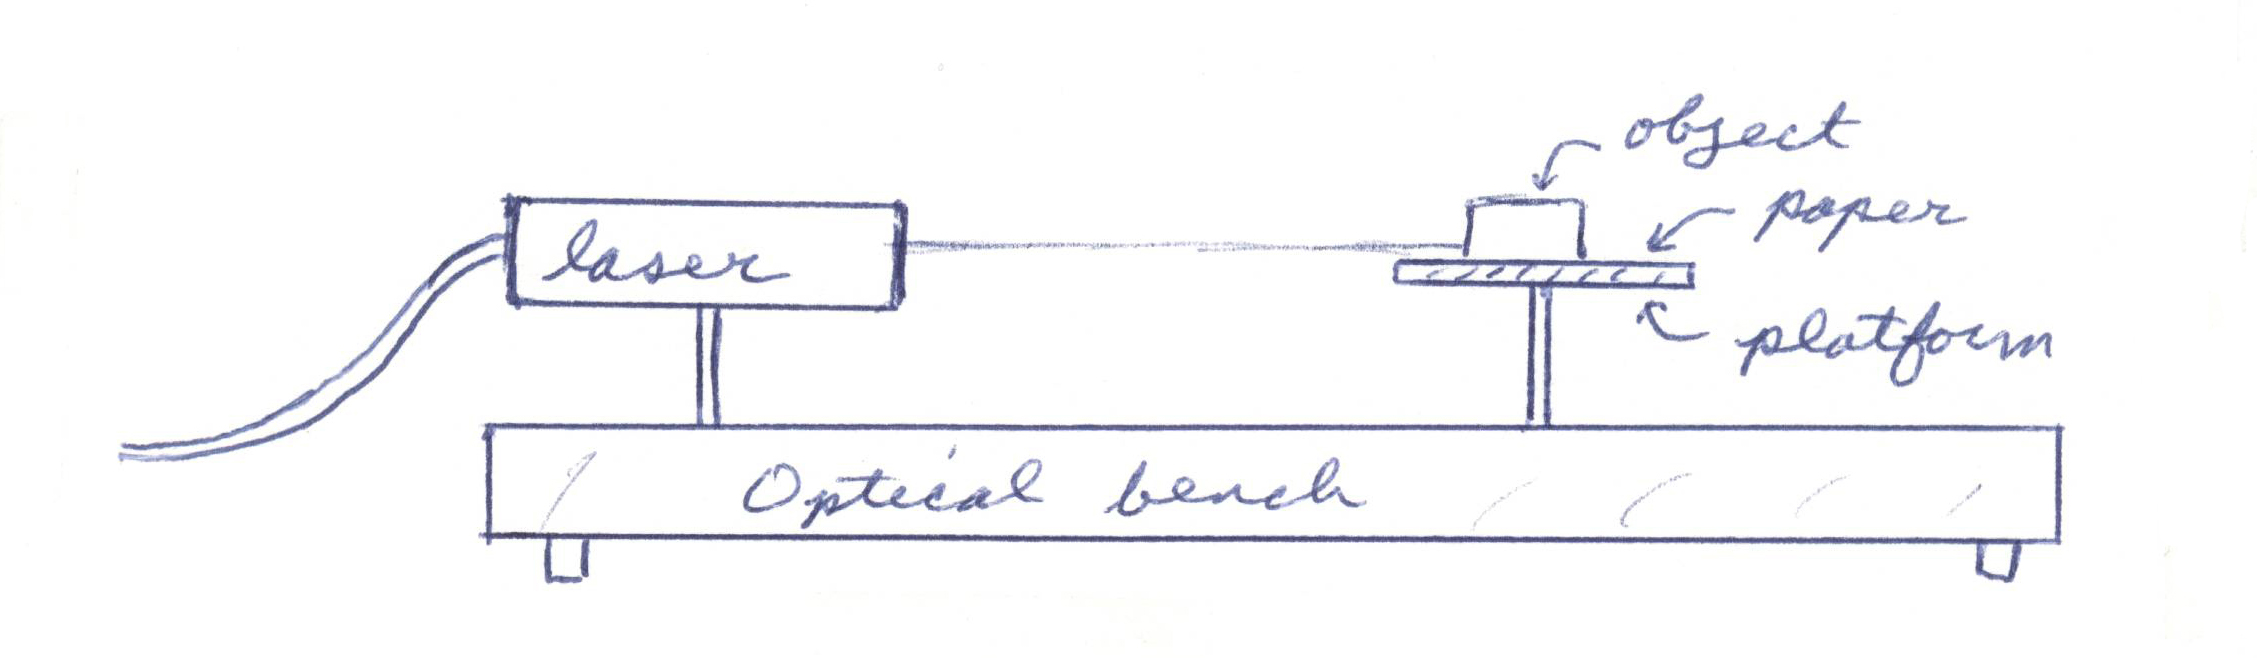
\includegraphics[scale=0.8]{5bgraf/fig_14}
	\caption{Laser on optical bench}
	\label{f:fig14}
\end{figure}

An optical bench is used to provide firm support for the laser and the platform on which measurements are made.  Align the laser and platform so that the beam is parallel to the surface of the platform.  Place a cork pad on the platform and a sheet of paper on top of the cork.  Pins placed judiciously can then be used to trace the path of the laser beam.

The law of reflection is particularly simple.  It is illustrated in the fig. {\ref{f:fig15}  The angle of incidence $\theta_i$ equals the angle of reflection $\theta_r$.  The law of refraction governs the direction of light rays when their speed changes, as in passing from one medium to another.  It is illustrated in fig. \ref{f:fig16}.  The equation for the law of refraction is called Snell's law and is written
\begin {equation} \label{e:snell}
n_1 \ \text{sin} \ \theta_1 = n_2 \ \text{sin} \ \theta_2
\end {equation}

where $n_1$ and $n_2$ are the indices of refraction for the media involved.  

%\begin{comment}
%\begin{figure}
%	\centering
%	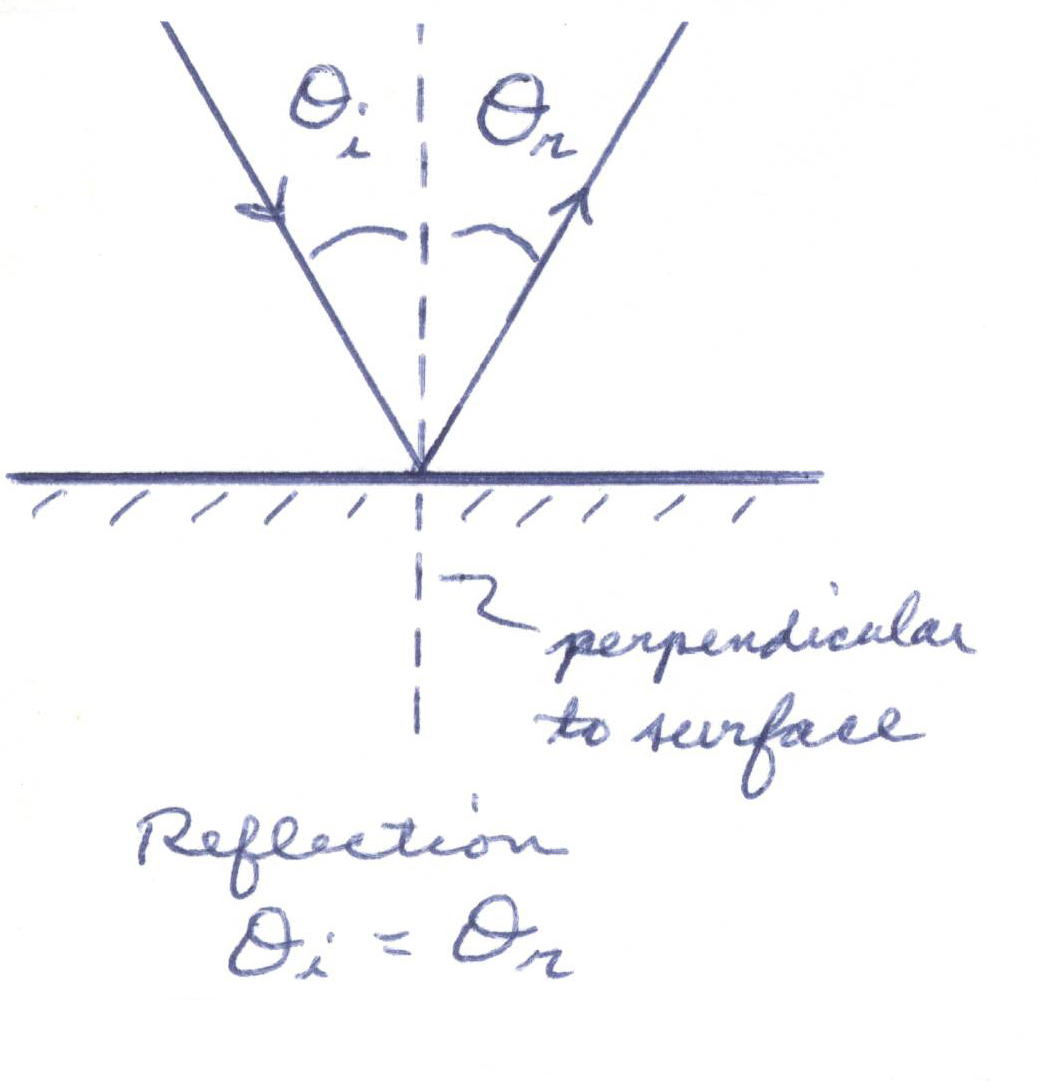
\includegraphics[scale=0.8]{5bgraf/fig_15}
%	\caption{Law of reflection}
%	\label{f:fig15}
%\end{figure}

%\begin{figure}
%	\centering
%	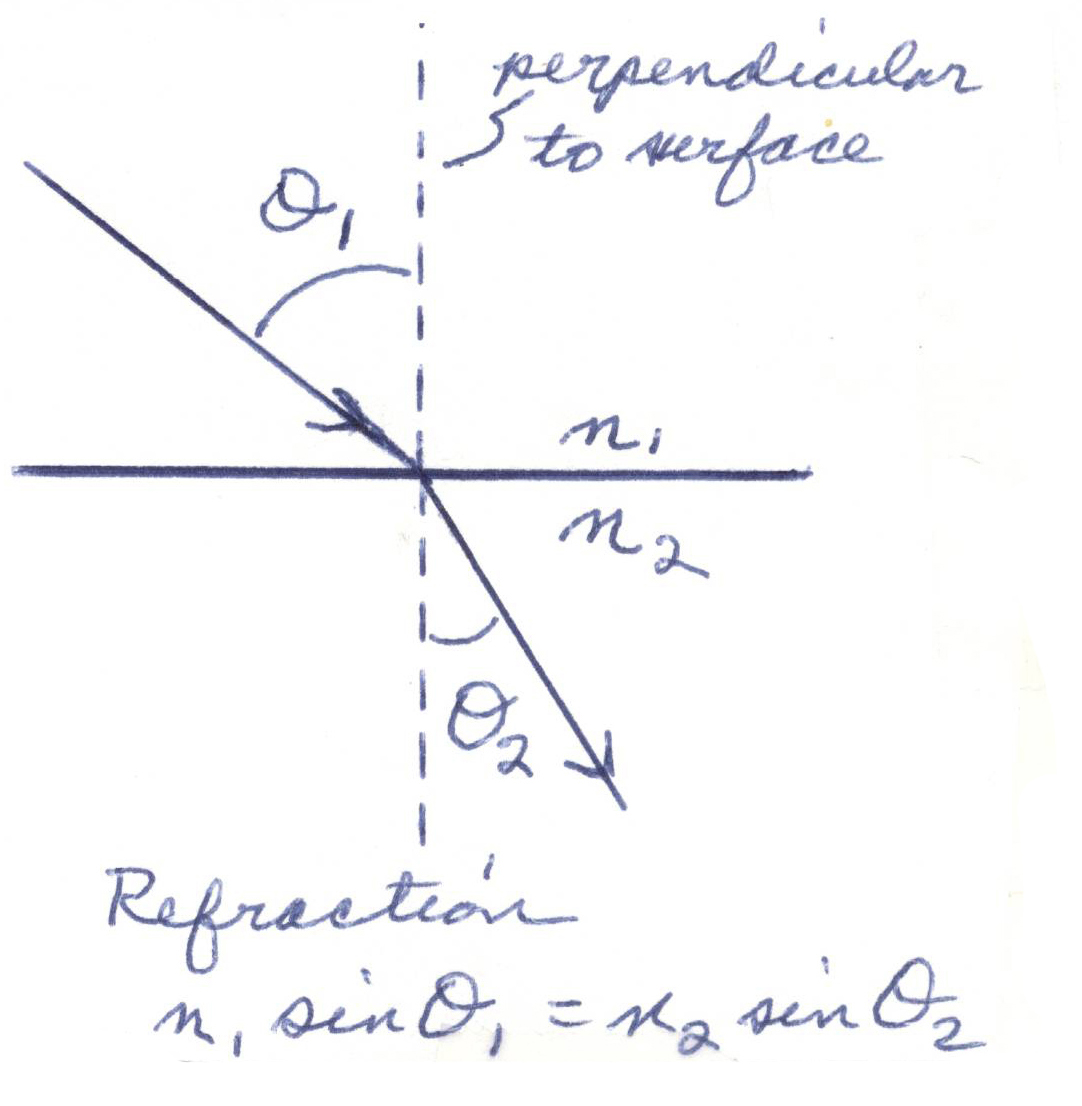
\includegraphics[scale=0.8]{5bgraf/fig_16}
%	\caption{Law of refraction}
%	\label{f:fig16}
%\end{figure}
%\end{comment}

\begin{figure} \centering
 \subfloat[reflection]
   {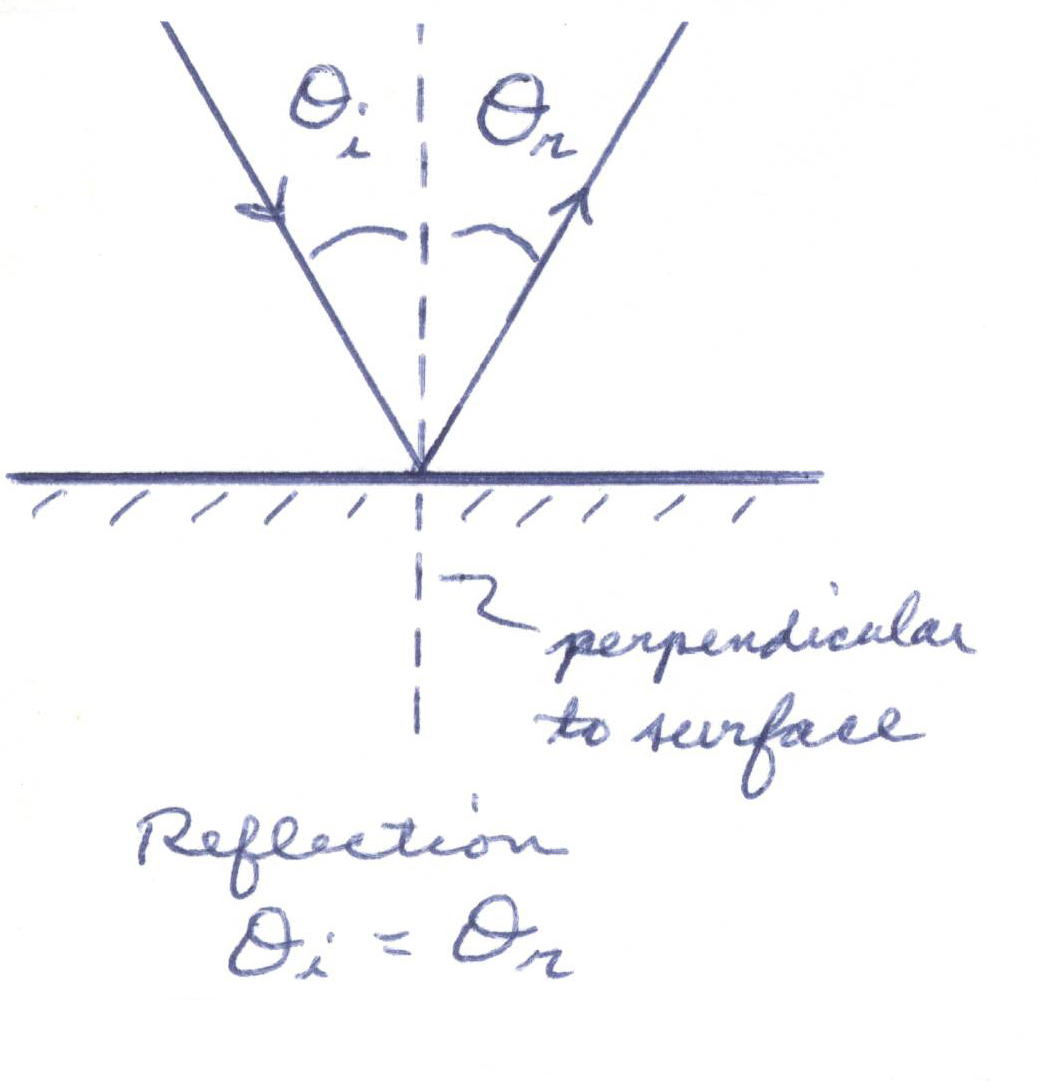
\includegraphics[scale=0.9]{5bgraf/fig_15}\label{f:fig15}}
 \qquad \qquad
 \subfloat[refraction]
   {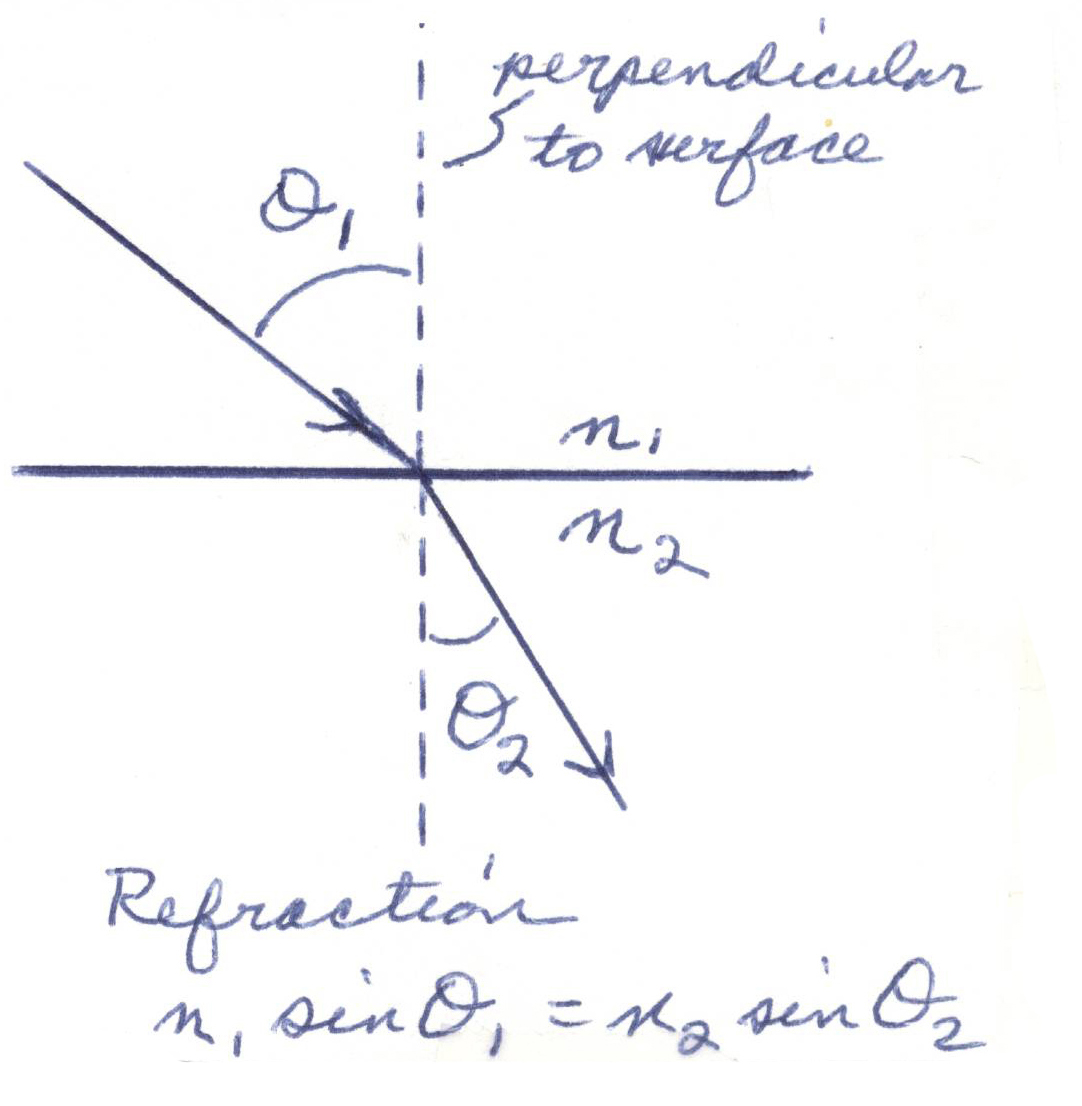
\includegraphics[scale=0.9]{5bgraf/fig_16}\label{f:fig16}}
 \caption{Laws of Reflection and Refraction}\label{f:rfract}
\end{figure}

Note that the angles are measured relative to a line that is perpendicular to the surface at the point where the light ray meets the surface.  The perpendicular is shown as a dashed line.  You can use a protractor to draw the perpendicular.  Your instructor will guide you in both determining the perpendicular and measuring pertinent angles.

\section{Geometric optics: ray model}

\subsection{Activity: Reflection and Refraction}
\begin{enumerate}
% Verify the law of reflection
	\item Use the front silvered mirror to verify the law of reflection.  Make measurements for three different angles of incidence.  Discuss whether the law is verified within experimental uncertainties.

% Verify the law of refraction
	\item Partially fill the pie box with water and a small amount of powdered milk. Trace a ray of light as it enters and leaves the pie box.  
	\item Taking the index of refraction of water to be 1.33 and that of air to be 1.00, check to see if the law of refraction (Snell's law: eqn.\ref{e:snell}) is verified at both the entry and exit points.  As usual, the verification need only be within experimental uncertainties.
	\item Discuss your results. Also discuss why your results are not affected by the fact that the light goes through plastic as well as air and water.
\end{enumerate}
	
\subsection{Activity: Index of refraction of glass}
Trace a ray of light through a glass block and glass prism.  Using the law of refraction and your measured angles, find the index of refraction of the glass.  Take the index of refraction of air to be 1.00.  How does your value for glass compare with the values listed in your text?

\begin{equation} \label{e:critang}
	\theta_c = \sin^{-1} \left(\frac{n_2}{n_1}\right) \text{where} \ n_1 > n_2
\end{equation}
	 

\subsection{Activity: Critical angle for a glass-air surface}
Pass the ray of light through a prism.  Gradually rotate the prism so that the ray leaving the other side comes out at progressively greater angles relative to the perpendicular to the surface.  Determine at what internal angle the light no longer emerges.  The smallest such angle is the critical angle.  Compare your measured value with that calculated using equation \ref{e:critang}:

\subsection{Activity: Focal point and length}
%  Find the focal point and focal length of a concave mirror
\begin{enumerate}
	 \item 	Use the curved metal mirror to verify that the focal length of such a mirror is one half its radius of curvature.  Measure the radius of curvature $R$ of the mirror by tracing its curve with a large compass.  Then trace the paths of parallel incident rays before and after they are reflected by the mirror.  The point at which they cross after reflection is the focal point.  
	 \item Measure the distance of this point from the mirror.  This is the focal length $f$ of the mirror.  
	 \item Discuss whether $f$ is half the radius of curvature $R$, as is predicted by the law of reflection.
\end{enumerate}
	
\section{Conclusions}
  What general conclusions can you make concerning the laws of reflection and refraction based on your experiences in this lab?
 
% \clearpage
%\newpage
%\includegraphics*[width=\textwidth,trim=120 80 80 120,clip]{5bgraf/pslabgrid} 
 
%--------------------------------------------------------------------------
\endinput
%--------------------------------------------------------------------------
			%--lab 08-------------------------------------

%--------------------------------------------------------------------------
% !TEX root = 5Blman.tex
% lenses.tex
% 2013.01.07 changed to 2col format
%--------------------------------------------------------------------------
\chapter{Thin Lenses and Their Images}

\begin{multicols}{2}
%---------------------------------------------------------------------
\section{Purpose}
  The purpose of these laboratory exercises is to give you hands-on experience with thin lenses and the images they form. In this lab, you will also determine the focal length of a lens, determine image distances and magnifications, and verify the thin lens equation.
  
%\begin{wrapfigure}[13]{r}[90pt]{0pt}	
%  \centering
%  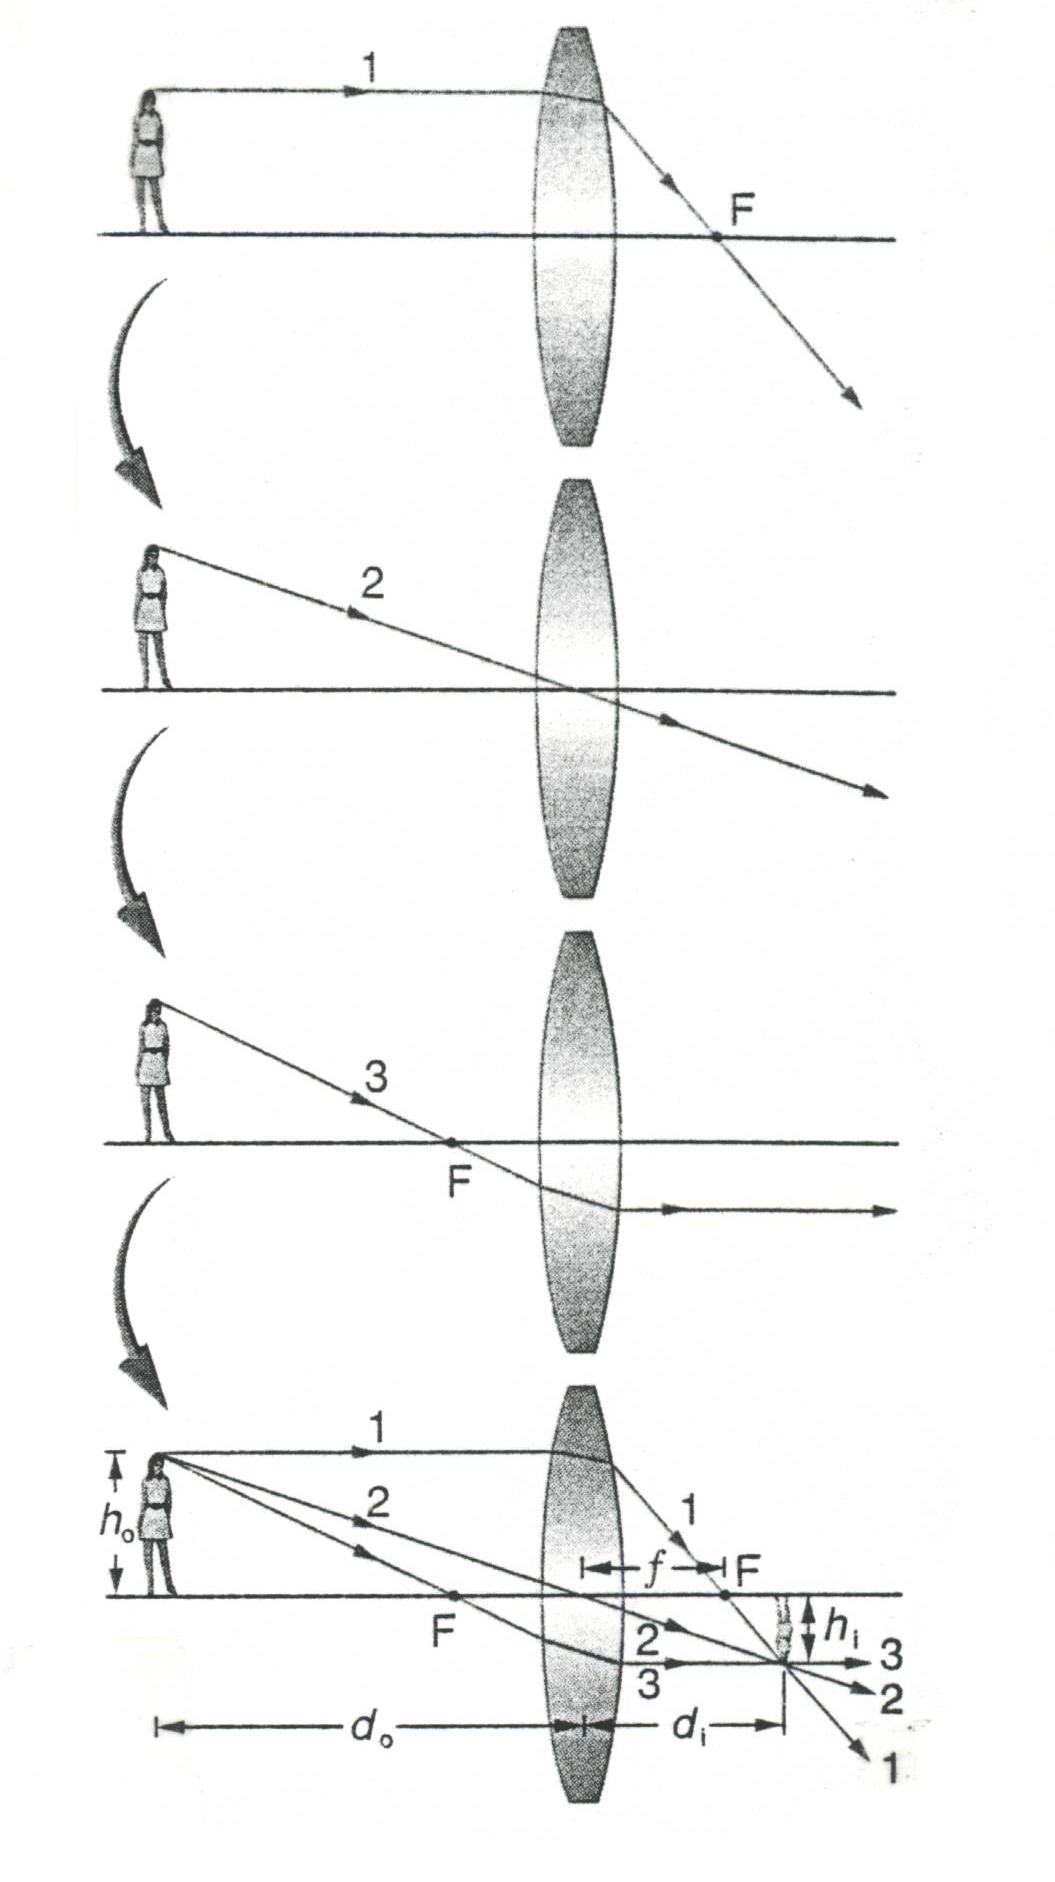
\includegraphics[scale=0.7]{5bgraf/fig_17}
%  \label{f:fig17}
%  \caption{Ray tracing}
%\end{wrapfigure}

%\parpic[r]{\fbox{\Large\scshape Box}}
%\newcommand\FIG{\includegraphics%		 set path on next line
%                 [scale=0.6]{5bgraf/fig_17}}
%                  [width=4cm]{5bgraf/fig_17}}
%                  [width=110pt]{5bgraf/fig_17}}
%\parpic[r]{\FIG}

% may get unpredictable behavior if order is not followed. Option cmds precede \parpic, followed by text. There should be enough text to 'cover' the figure.


%\piccaptiontopside
%\piccaption{Ray tracing} 
%\label{f:fig17}
%\parpic(4cm,6cm)(40mm,110mm)[r]{\FIG}
%\picskip{2}

%---------------------------------------------------------------------
\section{Preparation}
Reread the sections in your text on thin lenses.  Pay particular attention to the technique of ray tracing and the application of the thin lens equations for image formation by lenses.  Become familiar with the three types of images that can be formed by a single thin lens and the conditions under which each type is formed.

\paragraph{Short quiz}
  Be prepared to take a short quiz at the beginning of lab related to the concepts associated with this laboratory exercise.

%---------------------------------------------------------------------
\section{General Information}

%\piccaption{Ray tracing} 
%\label{f:fig17}
%\parpic(0cm,0cm)(40mm,70mm)[r]{\FIG}
%\picskip{2}

The technique of ray tracing is used to find the location and type of image formed by an optical system. In your text you will find several examples of ray tracing that are pertinent to this laboratory exercise. \reffig{f:fig17} shows a step-by-step illustration of ray tracing for a convex lens with an object at a distance greater than the focal length of the lens.  When ray tracing is performed carefully to scale it accurately predicts information about the size and location of images formed by optical instruments.

%\begin{figure}
%	\centering
%	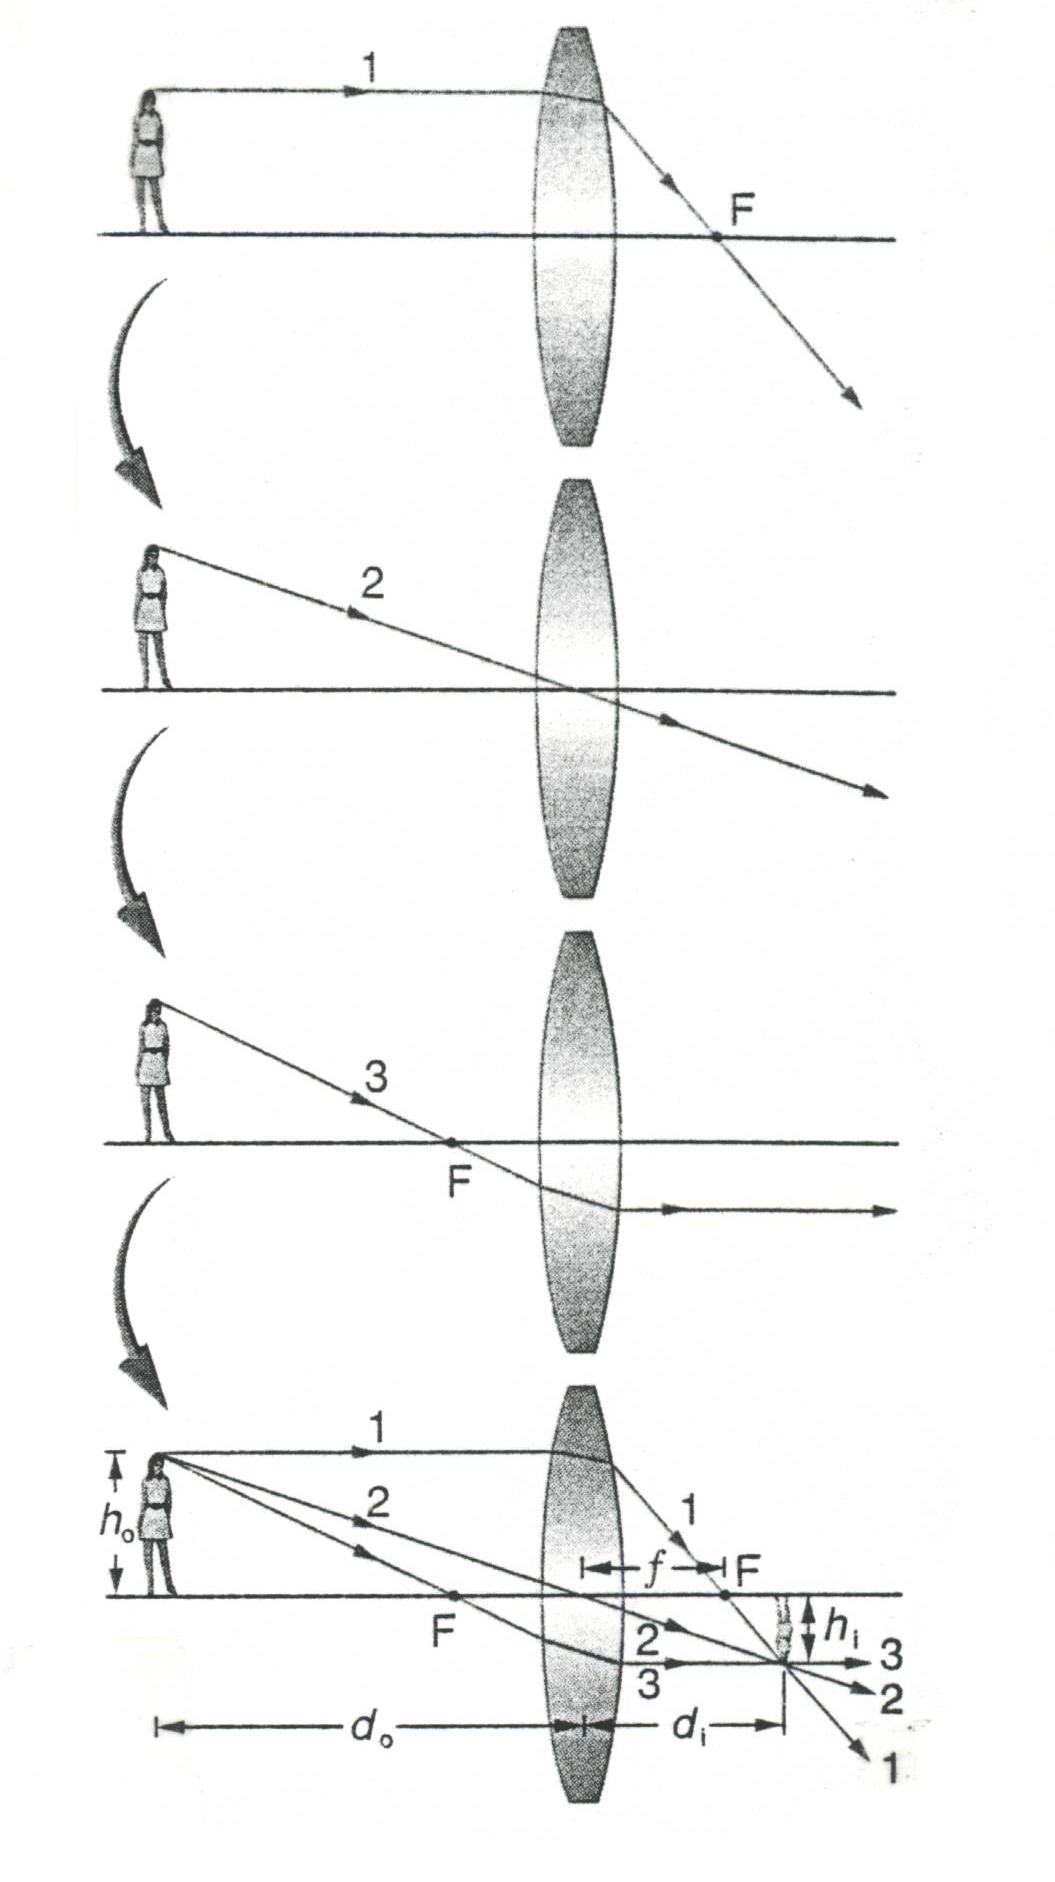
\includegraphics[scale=0.7]{5bgraf/fig_17}
%	\caption{Ray tracing is used to locate the image formed by a lens}
%	\label{f:fig17}
%\end{figure}

\begin{center}
	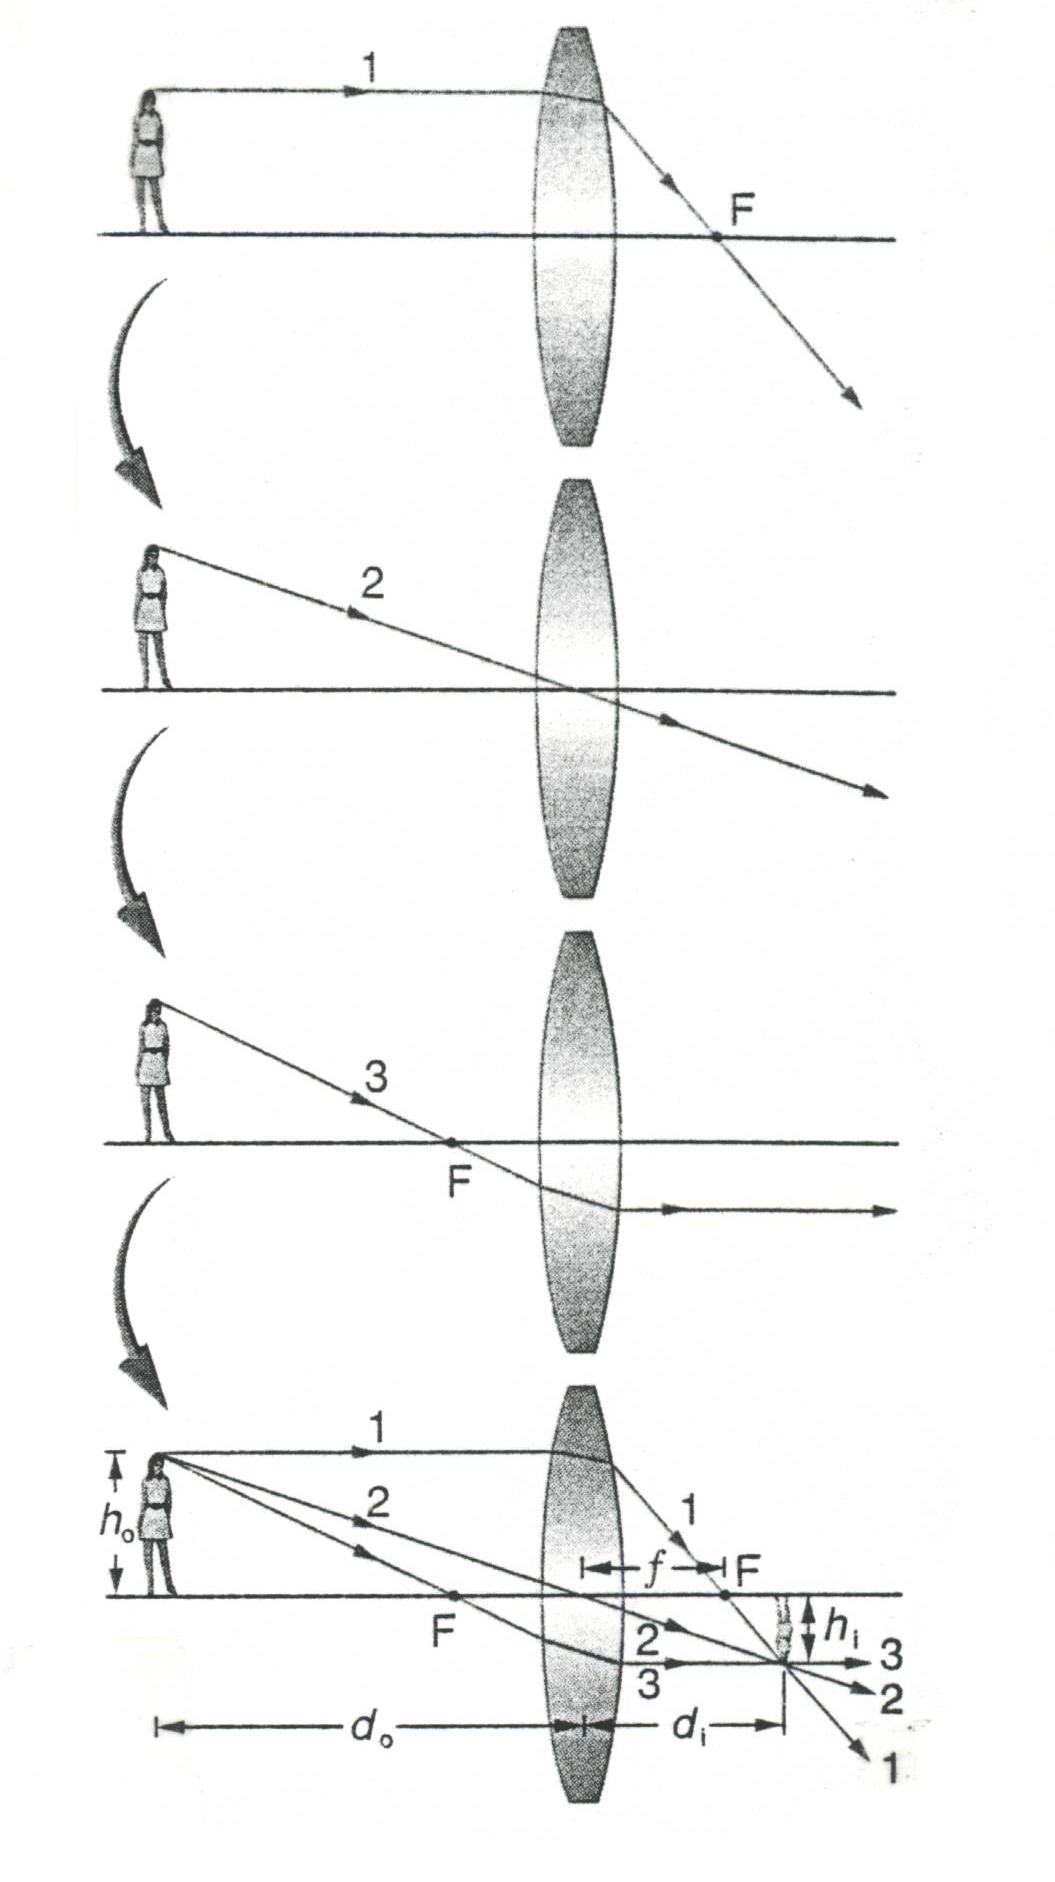
\includegraphics[scale=0.7]{5bgraf/fig_17}
	\mfcaption{Ray tracing is used to locate the image formed by a lens}
	\label{f:fig17}
\end{center}

The thin lens equations give the relationships of various quantities involved with thin lenses.  Note that the thin lens calculations produce results consistent with ray tracing and are in fact a numerical equivalent to the graphical techniques of ray tracing.

The object, $d_o$ and image, $d_i$ distances are related to the lens focal length $f$ by the thin lens equation, while the magnification is related to the distances, and to the image and object heights.

\begin{equation} \label{e:thin}
	\frac{1}{d_o} + \frac{1}{d_i} = \frac{1}{f}
\end{equation}
and
\begin{equation} \label{e:thinmag}
	\frac{h_i}{h_o} = -\frac{d_i}{d_o} = m
\end{equation}

\paragraph{Note} Your textbook may use different names for object and image distances, such as $p$ and $q$, or $s$ and $s'$.

%---------------------------------------------------------------------
%\section{Activities}
\section {Thin lenses}
\subsection{Activity: Focal length of a convex lens}\label{s:focal}
\begin{enumerate}[leftmargin=*] 
	\item Determine the focal length $f$ of a convex lens by forming an image of a distant object.  The object should be something you can see out the lab window.
	\item Explain your technique and estimate the uncertainty in your value for $f$
\end{enumerate}

\subsection{Activity: Images formed by a single thin lens}\label{s:thinlens}
\begin{enumerate}[leftmargin=*] 
	\item Using the optical bench, the light source, and the hooded screen, find the image location experimentally for the six situations below. For the first five, use the converging lens whose focal length $f$ you measured in activity \ref{s:focal}. Make a table in which you list values and uncertainties for the measured quantities $d_o$ (cm), $d_i$ (cm), $h_o$ (cm), $h_i$ (cm), and  $m$ for each of the five situations.
	\item Make room in your table for two other columns -- one for the calculated value of $d_i$ (cm) and another for the calculated value of $m$.
\end{enumerate}
	
\hrule	
\begin{equation*}
\begin{array}{llll}
	\text{(i)}	& d_o > 2f		& \text{(ii)}	& d_o = 2f \\
	\text{(iii)}	& f < d_o < 2f	& \text{(iv)}	& d_o = f \\
	\text{(v)}	& d_o < f 		& \text{(vi)}	& \text{any}\  d_o, \text{negative}\  f
\end{array}
\end{equation*}
		
\subsection{Activity: Image location using thin lens equation}
\begin{enumerate}[leftmargin=*] 
	\item Using the thin lens equation and the measured values of $d_o$ and $f$, calculate the location of the image $d_i$ in each of the first five situations. 
	\item Using the calculated value of $d_i$, find the magnification $m$. Include these calculated values in the table you made above. 
	\item Discuss how well the calculated values match the corresponding measured values. 
	\item In the sixth situation, calculate the focal length of the diverging lens.
	{\item (Measuring the image distance and location is difficult for the sixth situation, and is usually done using the ``parallax'' method, which your instructor will explain to you.)}
\end{enumerate}

\subsection{Activity: Ray tracing}
\begin{enumerate}[leftmargin=*] 
	\item For each of the six situations explored above, draw ray diagrams approximately to scale. Use graph paper, ruler, and thin lines to get the best results. Discuss any trends you observe. 
	\item Note the correspondence between the ray diagrams and the quantities measured in activity \ref{s:thinlens}.
\end{enumerate}

%---------------------------------------------------------------------
\section{Conclusions}
Did you observe the three types of images that can be formed by a single lens? Which of the six situations produced real images? Which produced virtual images? Which produced no image?  

% Questions: State what happens to the image distance as the object distance moves toward the focal point. Assume the object starts at infinity. State what happens to image distance as the object distance moves closer to the lens surface. Assume the object starts at the focal point.

% \clearpage
%\newpage
%\includegraphics*[width=\textwidth,trim=120 80 80 120,clip]{5bgraf/pslabgrid} 
 \end{multicols}
%--------------------------------------------------------------------------
\endinput
%--------------------------------------------------------------------------
			%--lab 09-------------------------------------

%--------------------------------------------------------------------------
% !TEX root = 5Blman.tex
% vision.tex
%--------------------------------------------------------------------------
\chapter{Vision}

\section{Purpose}
The purpose of this laboratory exercise is to explore image formation by the human eye. Adaptation of the eye for distant and close vision and the correction of the two most common vision defects will be explored.

\section{General Information}
Your instructor will explain the features and operation of the model eye. Some notable aspects: There are three positions for the retina. When the retina is positioned closes to the cornea, the eye becomes far sighted; in the center position the eye has normal vision and with the retina in the farthest position they eye is nearsighted. Close and distant vision are accomplished by placing two different lenses inside the eye. The $+7.0D$ lens is for distant vision (totally relaxed eye) and the $-20D$ lens is for close vision (fully accommodated eye).
The thin lens equations can be used for the eye, taking the cornea and internal lens of the eye to be a single thin lens. We will concentrate mainly on the first of those two equations:

\begin{equation}
	P = \frac{1}{d_0} + \frac{1}{d_i}
\end{equation}

\noindent where P is the dioptic power of the eye, $d_o$ is the distance to an object and $d_i$ is the distance to the image. Since it is difficult to determine where a single equivalent lens would be positioned, there is considerable uncertainty in measuring $d_o$ and $d_i$. The same thin lens equation can be used for a spectacle lens. The total dioptic power of the eye plus spectacle lens is approximately
	$P_{total} = P_{eye} + P_{spect}$.
	 
\section{The Human Eye}

\subsection{Activity: Role of water in the eye}
Role of water in the eye (aqueous and vitreous humors).
\begin{enumerate}
	\item With the $+7D$ lens in place and the retina in the center position (normal eye, completely relaxed) find the object distance that produces a clear image of the retina with no water in the eye.
	\item Fill the eye with water leaving the $+7D$ lens in place and find the object distance for which there is a clear image on the retina.
	\item Discuss the role of fluids in the eye. For example, explain what aspect of the anatomy of the eye (size, shape) necessitates the fluids. Also explain what effect these fluids have on the dioptic power of the eye (as compared to the eye with no fluids)
\end{enumerate}

\subsection{Activity: Accommodation of the normal eye}
The normal eye has the retina in the center position.
\begin{enumerate}
	\item Determine the lens to retina distance or $d_i$. (Note that to have a clear image of the retina di must equal the lens-to-retina distance.
	\item Measure (or estimate the case of distant vision) the object distances for the relaxed and accommodated eye. (As stated above, the relaxed eyes has the $+7 D$ lens in place while the accommodated eye has the $-20 D$ lens instead.)
	\item Calculate the dioptic power of the eye in both cases. That is, calculate the dioptic power of the normal eye for close and distant vision.
Why must the eye change dioptic power in order to see clearly at different distances?
\end{enumerate}

\subsection{Activity: Farsightedness}
Place the retina in the forward position to make the model eye farsighted.(Correcting close vision).
\begin{enumerate}
	 \item The farsighted eye will need a spectacle lens in front of the cornea to have clear vision of an object at the closest distance found for the normal eye.
	\item Place an object at the smallest $d_o$ found for the normal eye above, You will note that it produces a blurry image on the retina. Find a spectacle lens that when placed in front of the cornea gives good close vision.
	\item Calculate $P_{total}$ the total dioptic power of the corrected eye using measured values of $d_o$ and $d_i$ . Then use the dioptic power of the fully accommodated eye found in part 2c and calculate $P_{spec}$ . How does this calculated spectacle power compare to the one that actually corrected the farsightedness of the eye?
	\item Discuss why a convex or converging lens is needed to correct farsightedness.
\end{enumerate}

\subsection{Activity: Nearsightedness}
Place the retina in the far position to make the model eye nearsighted. Correcting distant vision.
\begin{enumerate}
	\item The nearsighted eye will need a spectacle lens in front of the cornea to have clear vision of an object at the farthest distance found for the normal eye
	\item Point the eye at an object at the largest $d_o$ found for the normal eye above. You will note that it produces a blurry image on the retina. Find a spectacle lens that when placed in front of the cornea give good distant vision.
	\item Calculate $P_{total}$ the total dioptic power of the corrected eye using measured values of $d_o$ and $d_i$ . Then use the dioptic power of the relaxed eye found in part 2c and calculate $P_{spect}$ . How does this calculated spectacle power compare to the one that actually corrected the nearsightedness of the eye?
	\item Discuss why a concave or diverging lens is needed to correct nearsightedness
\end{enumerate}

\subsection{Activity: Role of the pupil size}
\begin{enumerate}
	 \item Place the retinal in the center position to return the eye to normal vision. Use the $-20 D$ lens for close vision and place the object to get a clear image on the retina. Insert the diaphragm immediately in front the the $-20 D$ lens and describe its effect on the brightness and sharpness of the image.
	 \item Why does the diaphragm have this effect?
\end{enumerate}

\section{Conclusions} Did your measurements confirm the general aspects of close and distant vision as well as correction of farsightedness and nearsightedness? What was the greatest source of experimental uncertainty in this experiment?

% \clearpage
%\newpage
%\includegraphics*[width=\textwidth,trim=120 80 80 120,clip]{5bgraf/pslabgrid} 
 
%--------------------------------------------------------------------------
\endinput
%--------------------------------------------------------------------------
			%--lab 10-------------------------------------

%--------------------------------------------------------------------------
% !TEX root = 5Blman.tex
% optical.tex
% 2013.01.06 changed to 2col format
%--------------------------------------------------------------------------
\chapter{Optical Instruments}

\begin{multicols}{2}
%---------------------------------------------------------------------
\section{Objective}
To apply the principles of angular magnification and lateral magnification to the astronomical refracting telescope and the compound microscope. Both the telescope and the microscope utilize the lens systems called the eyepiece (near the viewing eye) and the objective (near the object being magnified).

%---------------------------------------------------------------------
\section{The eyepiece} For this experiment the eyepiece will consist of a single converging lens which we will call a ``simple magnifier'' The simple magnifier magnifies an object by creating a virtual image which subtends a greater angle at the eye than the original object.

%\begin{figure} %{wrapfigure}[8]{r}[30pt]{3cm}	
%  \centering
%  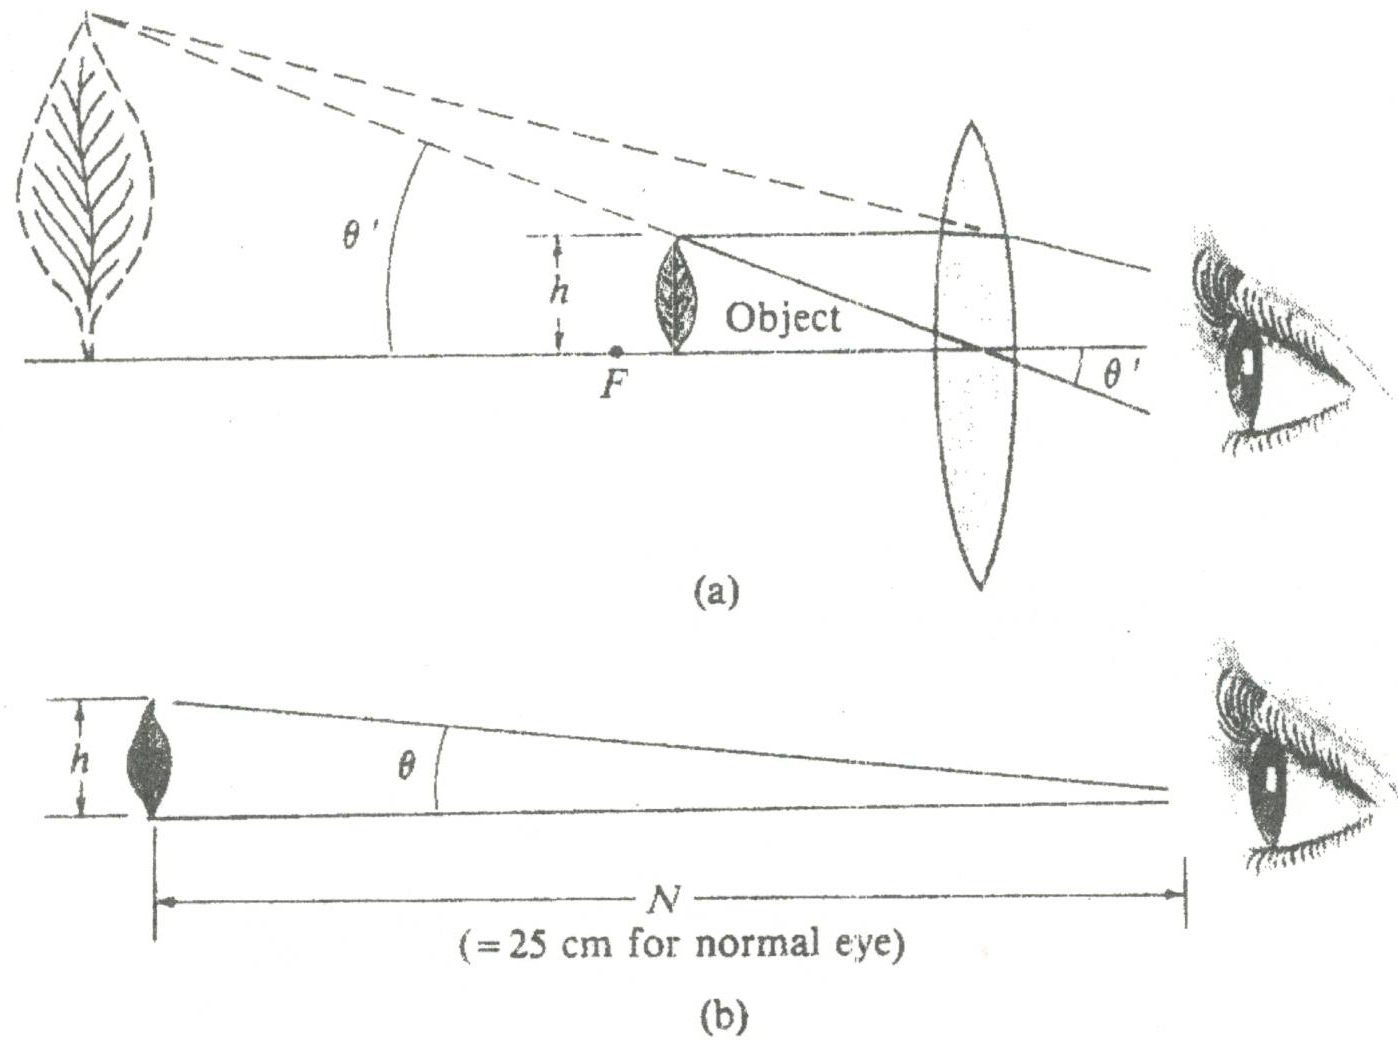
\includegraphics[scale=0.7]{5bgraf/mag}
%  \caption{Leaf viewed (a)through a magnifier (b)with the unaided eye}
%  \label{f:mag}
%\end{figure} %{wrapfigure}

\begin{center}
  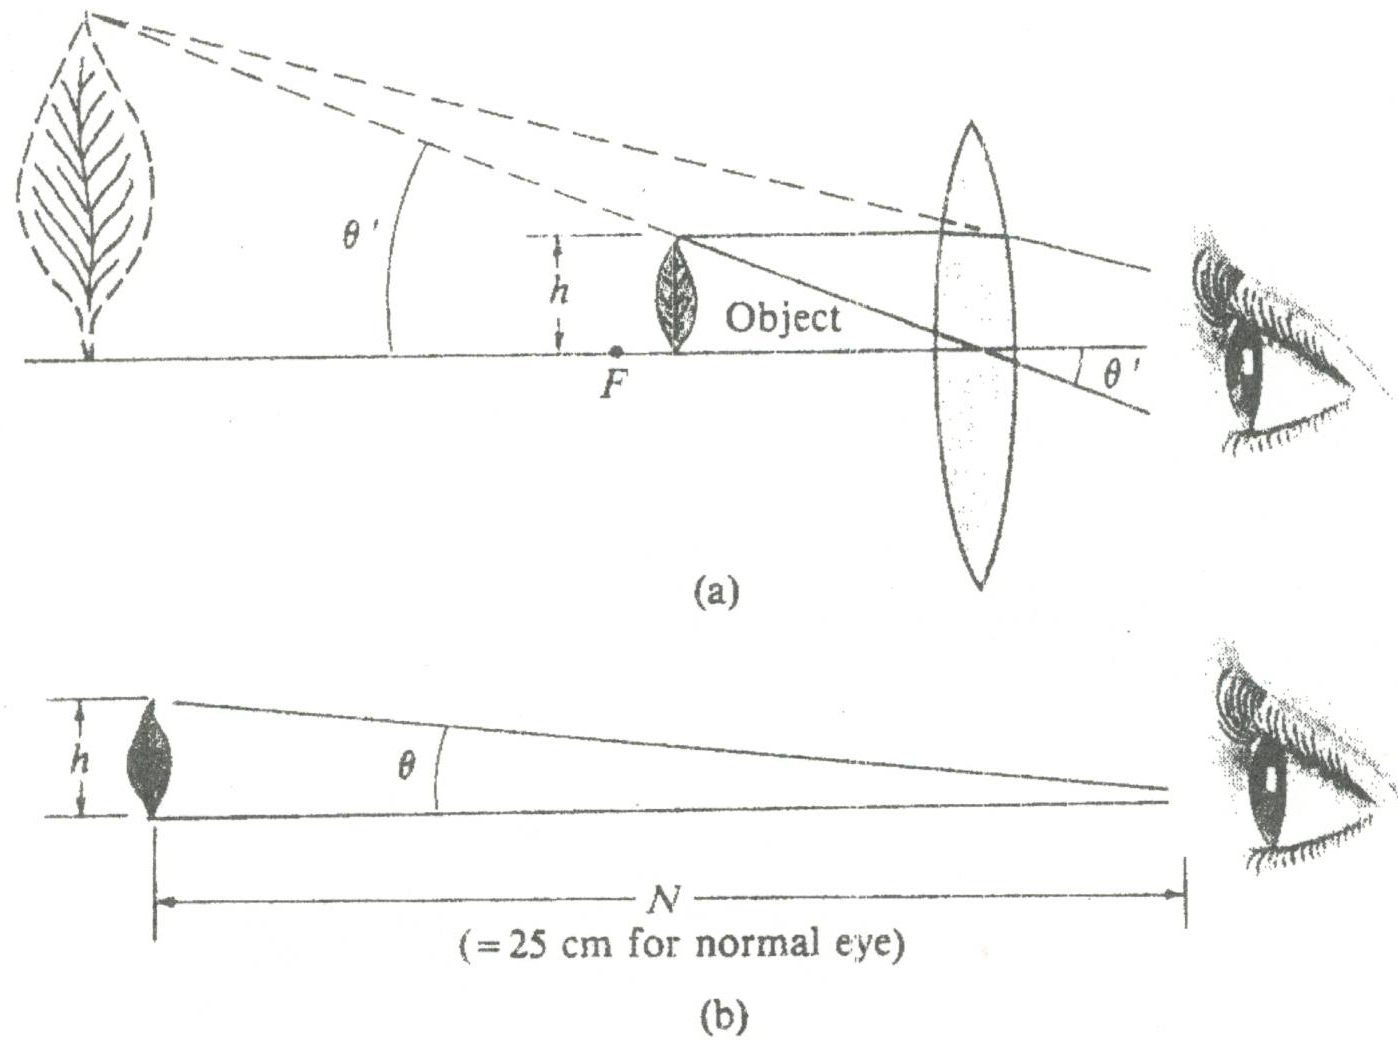
\includegraphics[scale=0.7]{5bgraf/mag}
  \mfcaption{Leaf viewed (a)through a magnifier (b)with the unaided eye}
  \label{f:mag}
\end{center}


This results in a larger image on the retina, hence the object ``appears'' larger. The amount the object appears to be larger is defined by the angular magnification or magnifying power of the lens.

For a normal eye (the near point, N = 25 cm)

% following are 3 methods to align math expression on more than 1 line
% alignment with the case environment
%\begin{equation}\label{e:mag}
%	M_{angular} = M_{eyepiece} =	
%	\begin{cases}
%		\frac{25}{f_e}		& \text {eye focused at infinity}\\
%		\frac{25}{f_e} + 1 	& \text {eye focused at near point (25 cm)}\\
%	\end{cases}
%\end{equation}

%% alignment with the array environment. specify #cols in array
%\begin{equation}
%	M_{angular} = M_{eyepiece} =
%	\left\{
%	\begin{array}{ll}
%		\frac{25}{f_e}		& \text {eye focused at infinity}\\
%		\frac{25}{f_e} + 1 	& \text {eye focused at near point (25 cm)}\\
%	\end{array}
%	\right.
%\end{equation}

% alignment with the alignedat environment. fractions are larger
\begin{equation}\label{e:mag}
	M_{angular} = M_{eyepiece} =
	\left\{
	\begin{alignedat}{2}
		&\frac{N}{f_e}		&& \quad\text {eye focused at infinity}\\
		&\frac{N}{f_e} + 1 	&& \quad\text {eye focused at near point}\\
	 \end{alignedat}
	\right.
\end{equation}


$f_e$ = focal length of the simple magnifier eyepiece

Note: Images formed by the eyepiece are virtual and upright, hence a simple magnifier can be used for reading purposes.

%---------------------------------------------------------------------
\section{The Refracting Astronomical Telescope}
A simple refracting telescope is illustrated in \reffig{f:tscope}

%\begin{figure}[htb] %{wrapfigure}[10]{r}[30pt]{3cm}	
%  \centering
%  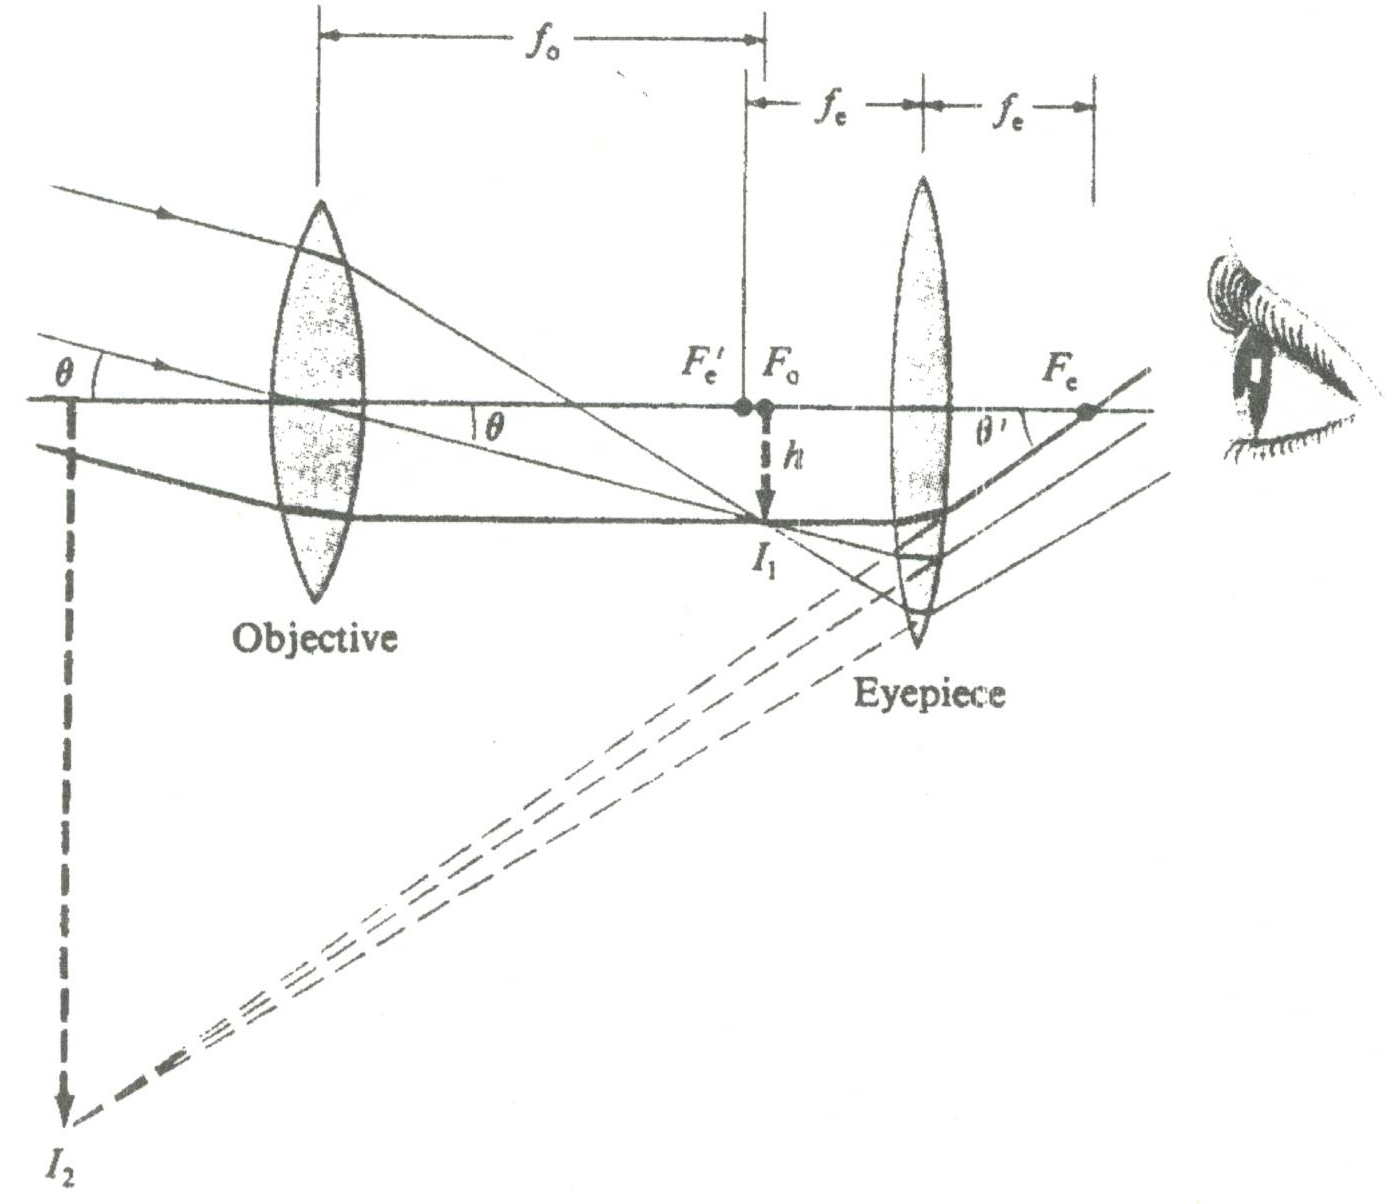
\includegraphics[scale=0.7]{5bgraf/tscope}
%  \caption{Refracting telescope}
%  \label{f:tscope}
%\end{figure} %{wrapfigure}

\begin{center}
  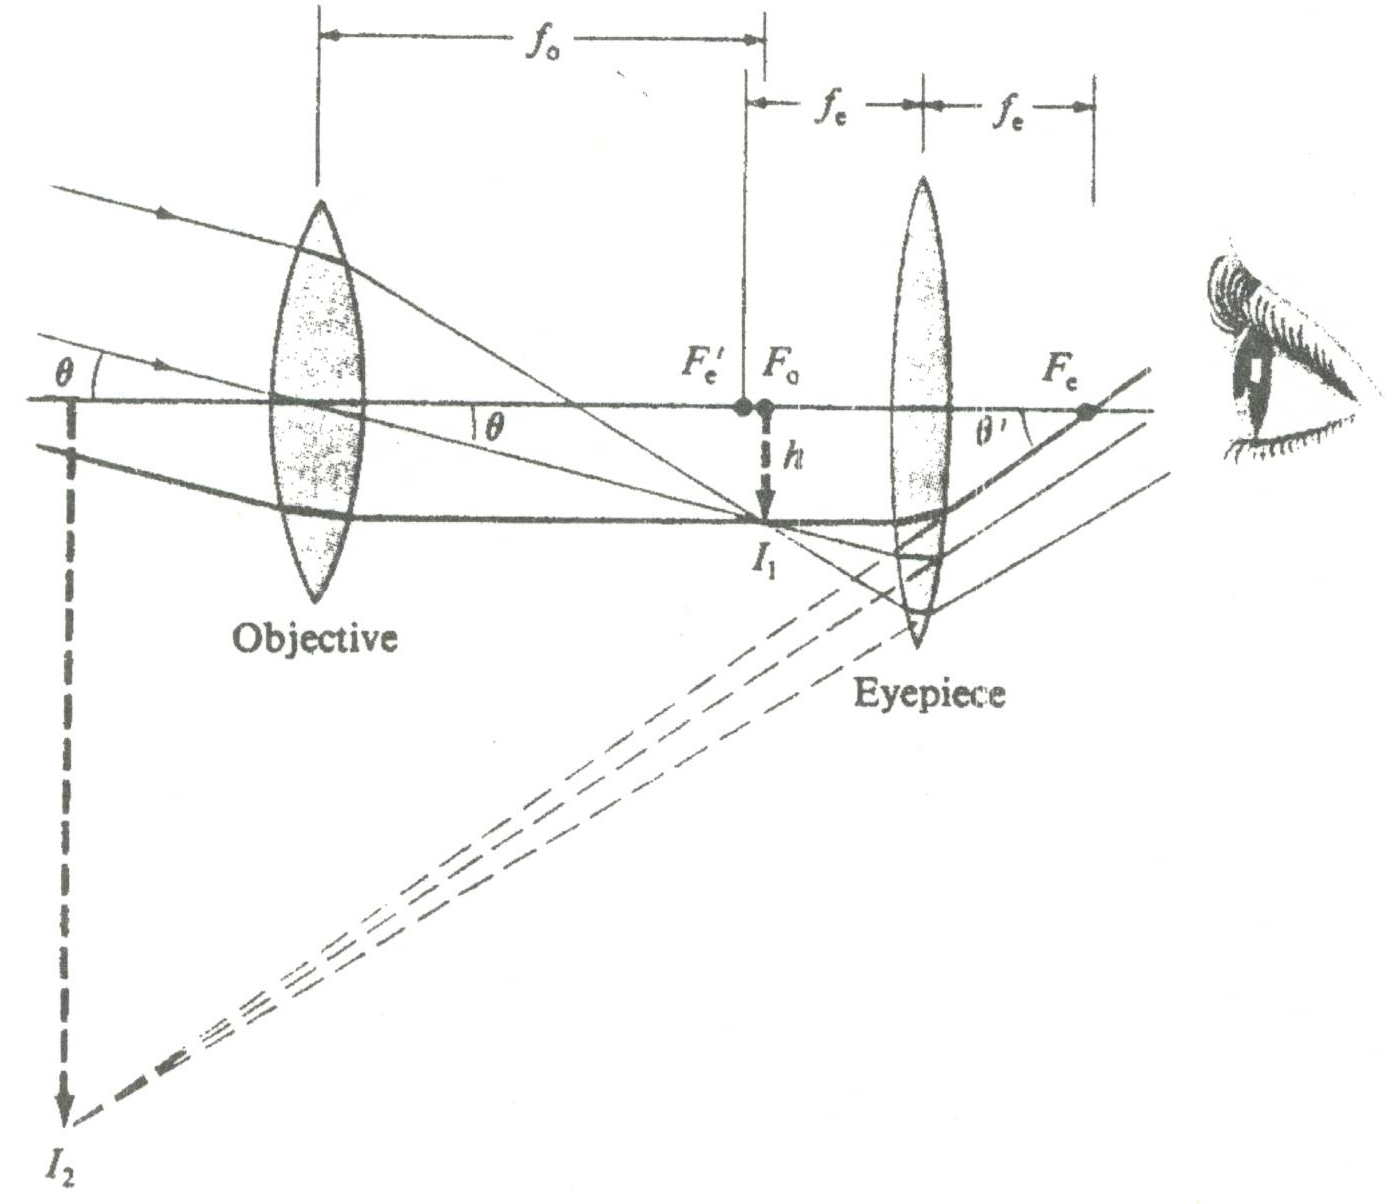
\includegraphics[scale=0.7]{5bgraf/tscope}
  \mfcaption{Refracting telescope}
  \label{f:tscope}
\end{center}


The features of this device are outlined as follows:
\begin{enumerate}
	\item The object is considered to be at infinity (very large distance). 
	\item The objective lens of focal length $f_o$ is of relatively large focal length.	
	\item The objective lens is a positive or converging lens.
	\item The objective lens forms a real, inverted image, which is then examined with the aid of the eyepiece lens, of focal length $f_e$. 
	\item The eyepiece lens is usually a short focal length lens.
	\item The eyepiece is then used to form a virtual image, at either the near point of the eye, or at infinity.
\end{enumerate}

Using trigonometric approximations you can confirm that the total magnifying power of this telescope is:
\begin{equation}\label{e:tscope}
	M = \frac{-f_o}{f_e}
\end{equation}
where the minus sign indicates that the image is `inverted'. It is assumed that the final image is at infinity.

\section{The Compound Microscope}
A simple compound microscope is illustrated in \reffig{f:mscope}:

%\begin{figure} [htb] %{wrapfigure}[8]{r}[20pt]{5cm}	
%  \centering
%  \includegraphics[scale=0.6]{5bgraf/mscope}
%  \caption{Compound microscope}
%  \label{f:mscope}
%\end{figure} %{wrapfigure}

\begin{center}
  \includegraphics[scale=0.6]{5bgraf/mscope}
  \mfcaption{Compound microscope}
  \label{f:mscope}
\end{center}


The features of this device are outlined as follows:
\begin{enumerate}
	\item The object is located close to, but just outside the focal point of the objective lens.
	\item The objective lens is a short focal length lens.
	\item The objective lens is a positive or converging lens. 
	\item The lateral magnification of the objective lens is
	\[
		M_o = \frac{L-f_e }{d_o}\approx -\frac{L}{f_o}
	\] 
	where $d_o$ is the object distance.
\end{enumerate}

Thus, the overall magnification of the microscope is
\begin{equation} \label{e:mscope}
	M = M_o \cdot M_e = -\frac{L}{f_o}\frac{N}{f_e}
\end{equation}


%---------------------------------------------------------------------
\section{Building optical instruments}
\subsection{Activity: Find the focal lengths}
\begin{enumerate}
	\item You have been provided with three lenses of different focal lengths.  Hold each lens up to a bright distant source of light (room lights out, focusing upon a distant object outdoors), and form a real image on a sheet of plain paper. Find, as accurately as possible, the distance from the image to the lens. This distance is a fairly accurate measure of the focal length of the lens. Recall that the focal length of a positive thin lens is that point where light from infinity is brought to focus. 

	\item Identify which lens you will use as an eyepiece or simple magnifier, and which lens will serve as an objective lens for the telescope and which for the microscope objective. Both the telescope and the microscope will utilize the same eyepiece lens.
\end{enumerate}

\subsection{Activity: Simple magnifier}
\begin{enumerate}
	 \item Mount a ruler in a vertical position on the optical bench. Use the simple magnifier to observe the magnified image of the ruler markings, as seen through the simple magnifier.
	 \item  Devise a way to measure the size of the image seen through the magnifier. Then compare the actual size of the ruler marking with the size as seen through the simple magnifier. 
	 \item Compare your experimental observations with that predicted from equations in \refeqn{e:mag}.
\end{enumerate}

\subsection{Activity: Build a telescope}
% On the optical bench, set up an astronomical telescope. Sight on a distant object (out the window or in the lab) of known or approximate size, and estimate the magnification observed. Compare with results predicted by equation \ref{e:tscope}.
 
\begin{enumerate}
	\item Mount your eyepiece and objective lens for your telescope on your optical bench. Remember that you need an objective lens with a long focal length for a telescope. The distance between your lenses should be about the sum of their focal lengths.
	\item Sight your telescope on a distant object (on the other side of the room or outside). You might need to adjust the separation of your lenses to get a good image. 
	\item Estimate the magnification of the image, and then compare your results with the expected angular magnification, predicted by \refeqn{e:tscope}.
\end{enumerate}

\subsection{Activity: Build a microscope}
%On the optical bench, set up a simple microscope. From the known size of the object, and the estimated size of the image seen, find the overall magnification produced. Compare your observed value with that calculated from equation \ref{e:mscope}. Make use of both values of possible magnification for the eyepiece.

\begin{enumerate}
	\item Mount your eyepiece and objective lens for your microscope on your optical bench. Remember that you need an objective lens with a short focal length for a microscope. The distance between your lenses should be longer than the sum of their focal lengths.
	\item Sight your microscope on a small object placed near the objective, just outside of the focal length of the objective. The distance scale on your screen is one possible object to start with. Again, estimate the overall magnification for your microscope and compare it with the expected value predicted by \refeqn{e:mscope}.
\end{enumerate}

%---------------------------------------------------------------------
\section{Question} 
The size of the image of Jupiter as seen through a telescope is definitely
smaller than the actual planet, ($h_{image} < h_{object}$ ), yet we say that the telescope has provided magnification. Explain what is being magnified.

\end{multicols}
%--------------------------------------------------------------------------
\endinput
%--------------------------------------------------------------------------
			%--lab 11-------------------------------------

%--------------------------------------------------------------------------
% !TEX root = 5Blman.tex
% interfere.tex
%--------------------------------------------------------------------------
\chapter{Interference and Diffraction}

\section{Purpose}  The purpose of these laboratory exercises is to give you hands-on experience with interference and diffraction effects produced by a double slit.
\section{Preparation}  Reread the section on interference and diffraction before coming to lab.  Pay particular attention to the conditions that produce constructive and destructive interference for light passed through a double slit.  We will also see evidence of single slit diffraction in the double slit pattern, so you should reread the relevant sections and carefully examine the figures in your text associated with the phenomena.

%\begin{wrapfigure}[7]{r}[0pt]{2cm}	
%  \centering
%  \includegraphics[scale=0.7]{5bgraf/fig_18}
%%  \caption{Double slit interference}
%  \label{f:fig18}
%\end{wrapfigure}

%\begin{figure}
\begin{SCfigure} % use sidecap pkg
	\centering
	\includegraphics[scale=0.8]{5bgraf/fig_18}
	\caption{Double slit interference}
	\label{f:fig18}
\end{SCfigure}
%\end{figure}

\section{General Information}
The figure shown is a schematic of the experimental set up for this laboratory exercise. There is a double slit at a distance $x$ from a screen.  When laser light is shown through the slit toward the screen a diffraction pattern will be observed.  Since the separation of the slits $d$ is relatively large compared to the wavelength  of the light used, there are a large number of bright dots where constructive interference occurs.  These are sometimes referred to as fringes.  Distance along the line of fringes is denoted by $y$. By using a little trigonometry and the small angle approximation, you find that the average distance between fringes under these circumstances is given by: 
\begin{equation} \label{e:deltay}
	\Delta y \approx x  \cdot \frac{\lambda}{d}
\end{equation}

You will measure $\Delta y$, $x$, and $d$ and equation (\ref{e:deltay}) to calculate a value for the wavelength $\lambda$ of a Helium Neon or diode laser. By rearranging the equation above you get:
\begin{equation} \label{e:lambda}
	\lambda \approx d \cdot \frac{\Delta y}{x}
\end{equation}

\section {Double slit interference}

\subsection{Activity: Double slit}
% Measure $d$, the double slit separation 
\begin{enumerate}
	\item Your instructor will guide you in adjusting the traveling microscope.  Make at least two measurements of $d$ for each of the double slits you use.  Estimate and record the experimental uncertainty in $d$.
	\item 	Mount the laser and double slit so that a diffraction pattern is produced on a wall at least 4 meters away.  Measure this distance (this is your experimental value of $x$) as accurately as you can.  As usual, estimate and record the uncertainty in this distance.
\end{enumerate}

\subsection{Activity: Wavelength of laser light}
% Record and measure the pattern of fringes
\begin{enumerate}
	 \item 	Place a piece of paper on the wall and record the location of as many fringes as possible.  Obtain the most accurate value possible for the average distance between fringes.  This is your experimental value of $y$.  Also estimate the uncertainty in your value of $y$.
	 \item Use equation (\ref{e:lambda}) above to calculate the wavelength of light used in this exercise.
	 \item Repeat the process for a second double slit having a different value of $d$.
	 \item Compare your results with the actual value for $\lambda$
	Calculate the percent difference between each of your experimental values for $\lambda$ and the actual value of 632.8 nm for a HeNe laser. The value for a diode laser will differ slightly.
	\item Determine if your experimental results agree with the actual value
	Calculate the percent uncertainties in $y$, $x$, and $d$ based on your estimated uncertainties.  Add the percent uncertainties and see if they are greater than the percent difference between your experimental value and the actual value.  Discuss whether or not you have agreement.
\end{enumerate}

\section{Activity: Single slit diffraction}
% Evidence of a single slit diffraction pattern in the double slit pattern
	Describe the evidence for single slit diffraction observed in the double slit pattern.

\section {Conclusions} What evidence did you see for the wave nature of light in today's experiment?  Did your results agree quantitatively or only qualitatively with theory?
 
%--------------------------------------------------------------------------
\endinput
%--------------------------------------------------------------------------
		%--lab 12-------------------------------------

%--------------------------------------------------------------------------
% !TEX root = 5Blman.tex
% optical.tex
%--------------------------------------------------------------------------
% !TEX root = 5Blab.tex
\chapter{The Hydrogen Spectrum}

\begin{multicols}{2}
%---------------------------------------------------------------------
\section{Purpose}
  The purpose of these laboratory exercises is to measure the wavelengths of hydrogen spectral lines in the visible part of its spectrum.  This will also provide you with further hands-on experience in observing interference and diffraction effects produced by a diffraction grating.

%---------------------------------------------------------------------
\section{Preparation}
  We use a diffraction grating in this exercise. Pay particular attention to the conditions that produce constructive interference for light passed through a diffraction grating.
  
%---------------------------------------------------------------------
\section{General Information}
The following explains how we can obtain wavelengths using the diffraction grating and how we can calculate those wavelengths from atomic theory.
When light is passed through a diffraction grating an interference pattern gives constructive interference at angles  related to the wavelength  of the light and the separation $d$ of the slits.  The equation for this is

\begin{equation} \label{e:nfere} 
	d\cdot \sin\theta = m\cdot \lambda, \quad m = 0, 1, 2, \dots
\end{equation}

In our experiment we will observe the first order spectrum; that is, the spectrum for $m = 1$.  You will find a value for $d$ and measure the angles  for the observable spectral lines from a hydrogen discharge tube.  Experimental values of  can then be calculated using \refeqn{e:nfere}.
Atomic theory produces the following equation for the wavelengths of light emitted by hydrogen atoms.  Theoretical values of $\lambda$ are calculated using the Balmer \refeqn{e:balmer}.

\begin{equation}\label{e:balmer}
	\frac{1}{\lambda}= R\left(\frac{1}{n_f^2}-\frac{1}{n_i^2}\right)
\end{equation}

where $R = 1.097 \times 10^7/m$ is the Rydberg constant.  The symbols $n_f$ and $n_i$ are positive integers that represent electron orbits in the hydrogen atom.  If an electron makes a transition between orbits then $n_i$ represents the initial orbit and $n_f$ the final orbit.  For light (EM radiation, actually) to be omitted $n_i$ must be greater than $n_f$.  Visible radiation is obtained for orbits that end in the second orbit where $n_f = 2$.  The values of $n_i$ can thus be 3, 4, 5, 6\dots .  This is called the Balmer series.

%---------------------------------------------------------------------
\section{Atomic Spectra}

\subsection{Activity: Spectrometer calibration}
% Calculate $d$, the separation or distance between slits.
\begin{enumerate}
	 \item 	Your grating has a label on it giving the number of lines per centimeter.  From this calculate the value of $d$, the distance between slits.
	 \item 	The primary function of the spectrometer is to measure the angles at which spectral lines occur.  Your instructor will give you directions for proper adjustment of the spectrometer so that you can obtain the most accurate angle measurements possible.
	 \item 	Place the grating in the center of the spectrometer with its lines (slits) vertical.  The slit of the collimator must also be vertical.  The grating must be perpendicular to the light coming from the collimator.
	\item Adjust the collimator slit size
	
	Look directly at the hydrogen discharge tube through the slit of the collimator.  Move the source if it is not directly in the middle of the slit.  Adjust the size of the slit until it is narrow enough to produce narrow spectral lines, but not so narrow as to reduce the intensity of light to the point where it is difficult to see with the eye.
	\item Align the hydrogen discharge tube with the collimator
	
	Place the hydrogen discharge tube in front of the slit of the collimator.  CAUTION:  Do not touch the high voltage connections or the discharge tube when the power is on.  The high voltage can shock you and the tube becomes thermally hot and can produce burns.
	
	\item Record the zero angle reading of the spectrometer
	
	When looking directly at the hydrogen discharge tube, the spectrometer is at 0 degrees according to  \refeqn{e:nfere} above.  Your instructor will help you to adjust the spectrometer so that it reads 0 degrees under this condition.
\end{enumerate}

\subsection{Activity: Measuring spectral lines}
\begin{enumerate}
	\item Examine the scales and vernier for measuring angles
	
	The most difficult part of this lab is to properly measure angles.  Carefully examine the angular scales and the vernier scales on the spectroscope.  Note that you will measure minutes of arc (there are 60 minutes per degree) rather than decimal fractions.  Ask your instructor for guidance if you are uncertain how to read the scales.
	\item Measure angles for the first order hydrogen spectral lines
	
	Move the telescope to one side and observe the first order spectrum.  You should be able to see three lines easily and perhaps a fourth with some difficulty.  The colors of the lines are red, green, blue-green, and violet.  Note that the dimmer lines may not appear to have the proper color since color vision fails for dim light, so the blue-green may appear violet and the violet may look gray.  Make the cross hairs in the telescope fall in the middle of each line and record the angle observed.
	\item Repeat the measurement of angles on the opposite side
	% Measure and record the angles as above, but on the other side of zero.
\end{enumerate}
	
\subsection{Activity: Calculating spectral lines}
\begin{enumerate}
	\item Calculate the experimental values for the wavelengths
	
	Average the two angles obtained for each line and then use \refeqn{e:nfere} to calculate the wavelength.  Estimate the experimental uncertainties in $d$ and find the total percent uncertainty in each.  Add these percent uncertainties to obtain the total percent uncertainty in your measurements.
	\item Calculate the theoretical values of the wavelengths
	
	Using \refeqn{e:balmer} calculate the theoretical values of the wavelengths of the first four lines in the Balmer series.  These have $n_f$ = 2 and $n_i$ = 3, 4, 5, and 6.
	\item Compare experiment and theory
	
	Find the percent difference between the experimental and theoretical values for each of the wavelengths observed. Determine and discuss whether there is agreement within experimental uncertainty. 
\end{enumerate}
\end{multicols} 
%---------------------------------------------------------------------
\section{Conclusions}
Did today's laboratory exercise succeed in giving you a feeling for interference produced by diffraction gratings and their use as a spectroscopic tool?  What other conclusions can you reach regarding this laboratory exercise?

% \clearpage
%\newpage
%\includegraphics*[width=\textwidth,trim=120 80 80 120,clip]{5bgraf/pslabgrid} 

%--------------------------------------------------------------------------
\endinput
%--------------------------------------------------------------------------
		%--lab 13-------------------------------------

%--------------------------------------------------------------------------
% !TEX root = 5Blman.tex
% nuclear.tex
%--------------------------------------------------------------------------
\chapter {Nuclear Decay and Half-Life}

\section {Purpose} The purpose of these laboratory exercises is to observe the penetrating ability of three types of nuclear radiation and to measure the half-life of a radioactive substance.

\section {Preparation} Your lab instructor will introduce pertinent concepts at the start of the laboratory period.

\section {General Information}
Do not eat or drink during this laboratory. Wash your hands after you leave the laboratory. Although the radioactive sources are sealed, as an extra precaution we handle them only with the tweezers provided. Your instructor will explain the hazards of nuclear radiation and the proper procedures for radiation protection.

\section {Nuclear decay}

\subsection{Activity: Geiger counter}
\begin{enumerate}
	 \item Turn on the Geiger counter

Adjust the counter to the proper voltage as directed by your lab instructor. Do not exceed the recommended value

	\item Determine background counting rate
	
Do this by allowing the counter to run for two minutes and recording the number of counts. Do this at least three times and average the number of counts.

	\item Determine the ability of  $\alpha, \beta$, and $\gamma $ rays to penetrate materials

Place various absorbers between the source and Geiger counter until the radiation measured in a two-minute interval is reduced to background levels. Do this for each of the three sources provided.

	\item Explain the ability of radiation to penetrate materials

At the discretion of your lab instructor, you may be asked to explain why the different types of radiation have different abilities to penetrate materials.

\end{enumerate}


\subsection{Activity: Measuring the half-life of $^{115}In$}
% Measure the half-life of a radioactive source
Your instructor will explain how the source is created and discuss the meaning of half-life.
\begin{enumerate}
	\item Place the radioactive source in the apparatus as you did the $\alpha, \beta$, and $\gamma$ sources earlier in the lab.

	\item Count for at least 32 successive two-minute intervals, subtracting the average background contribution from each run.

	\item Determine the half-life by finding the time required for the counting rate to decline to one half some earlier value. Since the actual half-life is 54 minutes, you should be able to do this for three or four of your early two-minute counts. Average your values and compare the result with the actual value.
\end{enumerate}

\section {Questions and Conclusions}
Were you able to confirm the relative ability of $\alpha, \beta$, and $\gamma$ radiation to penetrate materials?

Did you see evidence that the half-life does not depend on when you start counting? How many half lives must pass before all of a radioactive source is gone? 
 
%--------------------------------------------------------------------------
\endinput
%--------------------------------------------------------------------------
			%--lab 14-------------------------------------
	 
%--Appendix------------------------------------------------------------
\appendix
%--------------------------------------------------------------------------
% !TEX root = 5Blman.tex
% labnotes.tex
%--------------------------------------------------------------------------
% 2012 Dec
% 2009 Jan. Instructor labnotes

\chapter{Instructor Labnotes}
%\begin{comment}
These notes from 5B were originally compiled to fill a void for instructors teaching the lab for the first time, or for instructors teaching it after a long hiatus when equipment, procedures, labs \dots may have changed. More importantly it is more a series of reminders and observations of some things to consider for the lab along with some suggestions how to get students through the lab. Over the years, a few labs have changed dramatically, others hardly at all. There are lots of places where the manual may lack clarity or sufficient guided assistance for students. Any suggestions you have about \emph{any aspect} of the manual will very likely be an improvement. So, let me (zn) know how your experiences can be incorporated into these notes or the manual itself.
%\end{comment}
%--------------------------------------------------------------------------
\section*{Introductory Lab}
The first lab is not assigned any particular activities. You may want to use it to check your registration roll and give students an idea of what to expect.

I usually stress that the lab is an important part of the course, but that it is not very tightly tied to the lectures nor to their textbook. Different instructors may be on different topics and the textbook may be ordered differently from the lab.

I find it a useful time to go over such things as course requirements, the lab schedule, grading, the lab report \ldots

Several labs refer to ``error and uncertainty analysis''. This would be a good time to let students know what you have in mind and define for them what you expect for error and uncertainty analysis. I try to keep it simple and give examples of percent difference and percent uncertainty. You will probably have to repeat your explanations several times during the semester, but at least students will have heard it a least once.

See Appendix \ref{a:rptformat} for a suggestion of a simple lab write up form. The sample focuses on four major parts of a report, the Introduction--Abstract, Preparation, Data Analysis--Observation, and Comment-Conclusion. It's really simple, but student always ask how should the lab be written up. I've tried many variations, including lab notebooks, but this simple form at least provides an answer to the question, ``What about lab reports''?
%--------------------------------------------------------------------------
\section{Lab 1 -- Electrostatics}
Results for this lab can literally vary with the weather. It might be overkill, but if students wash their hands before handling the equipment, this may decrease the amount of skin oils transferred to the cloths and rods. You may want to provide a brief explanation of the electroscope and warn students against overcharging them. Some of the gold leaves are damaged, so advise students to use the proof plane and show them how to use it when they are transferring charge directly to the electroscope.

A Van deGraft Generator and Wimshurst machine are placed in the lab if you want to use them. Both of them can be quite impressive as demos. I haven't done the hair raising demo in some time, but you will need an insulating platform to do it.

Students this early in the course may find electrostatic polarization and electrostatic induction confusing, even after your best explanations. I've found it useful to use step-by-step diagrams to highlight these phenomena as proceses and require students to do the same in their reports.

%--------------------------------------------------------------------------
\section{Lab 2 -- Electric Fields and Potentials}
For many students, this lab will be the first time they have ever used an electronic meter. To make things go more smoothly, I go into some detail to show them how to use the digital multimeter and explain what each button indicates. You'll probably have to repeat much of this again in later labs, but it will be good reinforcement. I've found that going through a dry run, then actually measuring, say the, voltage output of the VAC is useful. 

Let students know it's easier to outline the ``plates'' on the transparent plastic sheet before putting it in the tray. Then, students can tape the plastic grid sheet to the bottom of the tray, cover it with water, and ``squeegee'' out the bubbles. Alternatively, students can lay the plates onto the water covered sheet, then ``dimple'' an outline of the plates with the probe. It may help students to use the probes by guiding them through sample potential measurements, say at the equipotential line = 1 volt.

I have students do at least two configurations, and three if depending on time --- the parallel plate configuration, the dipole configuration (using the two round cylinders), and a choice using the parallel plates and a cylinder. As an additional learning aid, you may want students to display their samples on the projector and give a brief explanation of what they did, what they found, and how they interpret their results.

One last thing, I ask students to calculate the electric field $E = \Delta V/\Delta d$ for three locations between the parallel plates and one location outside the plates. It helps to do sample calculations on the board, as students may still have difficulty distinguishing between electric potentials, electric voltage, and electric fields.

%--------------------------------------------------------------------------
\section{Lab 3 -- Electrical Energy}
This lab uses an analog volt and current meter. You will probably have to explain how to use the meters, especially how to read the scales correctly. I work in the idea of ``parallax'' and emphasize how important it is to face the meter directly, rather than try to read it from an angle.

This might also be a good time to briefly introduce the idea of circuit diagrams by simply redrawing the block diagram as a schematic. One idea I stress for the next labs that use a voltmeter is this: \textsl{hook the voltmeter up last}. It's the easiest thing to hook up, but also the easiest thing to get wrong.

You may have to remind students to convert energy in cal to Joules (so that $E_{Thermal} \sim E_{Electrical}$), check and recheck the wiring before turning on the power, and keep the current constant at 2.2 A. For the last point, students often read the wrong scale (I refer to them as the 1 and 3 scale), so if their results are totally off, check how they read their current meter.

For the current semester (2010) the emphasis has changed slightly to focus on the mechanical equivalent of heat. You may still prefer to just compare the heat loss/gain in which students must convert the energy to \textsl{cal} or \textsl {J} for the comparison.

%--------------------------------------------------------------------------
\section{Lab 4 DC Circuits Part I}
Students will likely appreciate a brief discussion of the color code and how to read a resistor to obtain its resistance value. I suggest to students that they set up a table which has resistor values determined form (1) the resistor color code, (2) direct measurement of the resistor using an ohmmeter, and (3) calculation of the resistance using Ohm's Law.

You will probably have to explain again how to use the digital multimeter and the analog meter if you have not done it previously. This time students actually use the resistance measurement mode. Consider a sequenced exercise (or steps) that students perform directed by you in which they measure a battery voltage. Then they connect the resistor to a battery, a switch, and ammeter to measure the current. Finally, following the precept,\textsl{ hook up the voltmeter last}, use the voltmeter to measure the voltage across the resistor and across the battery. Hopefully, after this, students will feel more comfortable with using the equipment and doing so correctly.

As part of a pre-lab assignment to introduce students to the next lab (Lab 5: DC Circuits II) you might ask students to perform one or more of these tasks for the values given in the manual:
\begin{itemize}
	\item set-up a current equation at a junction
	\item set up two loop equations for voltage (the two ``inside'' loops and or the ``outside loop'') 
	\item solve the three equations for the unknown currents
\end{itemize}

%--------------------------------------------------------------------------
\section{Lab 5 DC Circuits Part II}
Students may find this lab difficult, especially if they are uncomfortable with multiloop circuits and the instruments. By this time, they might not have been introduced to Kirchoff's rules yet or had adequate time to use them in problems. A brief discussion illustrating Kirchoff's current and voltage rules using the lab circuit can help, including generation of the current and voltage equations.

Be aware that many students will try to ``compare'' the measured and calculated currents by simply placing the measured values into the circuit equations, then ``solve'' the equations, and note the both sides of the equations are unequal. There are lots of variations on this.  

%--------------------------------------------------------------------------
\section{Lab 6 Electromagnetic Induction}

%--------------------------------------------------------------------------
\section{Lab 7 Electromagnetic Radiation}
Although this is an exploratory lab, you still may want to have students turn in a lab write-up consisting of their observations, sketches, and comments. You should conduct the microwave demo for your lab section, guaranteeing that it will work at least once. The klystron tubes are old, get really hot, and their performance might fail at any time. As an exercise, I give students a set of numbers taken from a measurements of the maxima found when the hardboard is slid along the length between the two horns. From the results, I ask students to determine the wavelength of the microwave radiation and its frequency. [See Table: \ref{t:microwavepeaks} on page \pageref{t:microwavepeaks}].

\begin{table}[htbp]
\begin{minipage}{0.4\textwidth} 
\centering
\caption{Microwave Peak Signal} \label{t:microwavepeaks}
\begin{tabular}{l l l}\toprule
\# & X(cm) & Signal\\
\midrule
1.	&	2.84 &	max\\
2.	&	3.59 &	min\\
3.	&	4.31	 &	max	\\
4.	&	5.09 &	min\\
5.	&	5.86 &	max\\
6.	&	6.57	 &	min\\
7.	&	7.36 &	max\\
8.	&	8.14 &	min\\
9.	&	8.85 &	max\\
10.	& 	9.55 &	min\\
\bottomrule
\end{tabular}
\end{minipage} \hfill
\begin{minipage}{0.5\textwidth} 
	If you decide to use the values in the table, generate your own, or skip this entirely, be sure to explain to students how the wavelength and frequency can be determined.
\end{minipage}
\end{table}

%--------------------------------------------------------------------------
\section{Lab 8 Reflection and Refraction}

%--------------------------------------------------------------------------
\section{Lab 9 Thin Lenses}
I usually give a brief introduction to the lens equation, converging, and diverging lenses, and ray tracing.

You may want to demo how to use all the pieces in the tray to form an image. This goes quickly, which most students will figure out on their own.

I start out by having students determine the focal length of the converging lens by imaging an object "located at infinity", which for us is $\sim$100 times the focal length of the lens and more. For this, two light bulbs are set up at both ends of the lab. Students can use either bulb to ``image'' the bulb with their lens in a holder and measure the image distance - which is also the focal length in this case. 

Then I have them do it again. This time with the room still darkened, I open the blinds at the back of the room and ask students to image anything they can see outside the window. Many students may still be surprised that the image is upside down, even if you have already described the ray tracing.

However, finding the virtual image for a converging lens is not clear. I set up the ``light'' object inside the focal length of the lens then ask a volunteer to find the image on the side that students ``expect'' to find it. I also explain that this virtual image cannot be found or displayed on the screen where they expect to find  it. The image is on the ``other'' side, the side from which the light originates. I place a piece of paper or the screen on that side, and no one is hardly surprised that the image still does not appear, since the light source is blocked. Then I ask two or three students to peer through the lens looking toward the light source and describe what they see - which should be the enlarged image.

Only then do I launch into the explanation of the parallax method telling them to replace the ``light'' object (illuminated round and pointed arrows) with one of the metal pointers along the way. As they can ``see'' the image through the lens, the other pointer is used to find the location of the image. I suggest to them to set the ``image'' pointer a little higher than the ``object'' pointer. Looking through and around (or over) the lens they can sight the virtual image and the image pointer. Then move the image pointer forward and backward while moving their head slightly to the left and right. At some location they will see the image pointer and the image move in unison with each other rather than opposite directions. That location of the image pointer should be the location of the virtual image.

This can be both difficult to explain and to demonstrate. %So another method is suggested below which does not use parallax.

For the focal length of the diverging lens, have students put both lenses (converging and diverging} in one lens holder. The image will be real for the set of lenses we are using and the image distance will be much longer than students expect. So I encourage students to explore a little and try longer distance when they report they cannot see anything.


A few years ago C. Newcomb fashioned two pointers for use in determining the image of a virtual image for a converging lens. These two pointers are referred to as the ``straight'' (3--5 mm diameter by 5 cm rod) and ``bent pointer'' (3 -- 5 mm diameter by 9 cm rod with three right-angled bends). These should be better than the current pointers.

To find the image of a divergent lens,  I think it's better to separate the convergent and divergent lens by a constant distance $d$ then adjust the screen or lens distances until a real image appears. 

%--------------------------------------------------------------------------
\section{Lab 10 Vision}
%--------------------------------------------------------------------------
\section{Lab 11 Optical Instruments}

This lab uses three (3) converging lens with focal lengths which can be roughly described as short ($\sim$ 5 cm) , medium ($\sim$ 15 cm), and long ($\sim$ 27 cm).  Once students select the correct lenses for the three instruments (simple magnifier, telescope, and microscope) there is usually no problem in viewing the image. The problem is usually how to determine the image size from the physical set up.

I explain to students that they can look ``through'' and ``around'' the objective  lens at the same time. Then they can compare the number of say, lines of a ruler, seen through the lens with the number of lines of the ruler.

%--------------------------------------------------------------------------
\section{Lab 12 Diffraction and Interference}
In the past we have always done geometric optics (labs 8 -- 11) before wave/physical optics. Be prepared to make adjustments in case the order changes.

This lab uses the 1 mw HeNe laser. Students are suppose to measure the wavelength of this beam taking only measurements of the screen to length distance, the separation of the interference fringes, and the dimension of the slits.

Be aware that students often confuse the two pairs of slits as a ``double slit''. You might want to point this out to them and be sure that they distinguish the two slits. Also they should be able to tell, within a pair, what comprises the single slit and what comprises the double slit.

You will likely have to cover the operation and use of the linear microscope. Since this is the greatest source of uncertainty, it's important that students know how to use it. This can take a lot of time to explain and to demonstrate, which we don't have. At the minimum I let students know that the linear scale shows 1 cm divisions, 1 complete rotation on the rotary knob is 0.1 cm, and one unit division (say from 0 to 1 on the rotary knob) is 0.01 cm. Then I have students measure the diameter of a dot that they place on a piece of paper. First though, I have them adjust the scope so that the cross-hairs are in focus, then adjust the scope so that the image of the dot is in focus.

Measuring the slit width can be a problem. I suggest that students start at one edge of a pair of slits, record the location then slowly move to each each of the slit and record the location - so they'll have four locations, say 1, 2, 3, 4. They they can determine the slit separation $d$ by the values 3--1, and 4 -- 2.  The slit width, $D$ is then 2 -- 1, and 4 -- 3. Explain to them the problem of backlash and that they must always move in one direction.

To determine $\Delta y$, I suggest to students that they measure  the distance $y$ between $n$ bright fringes, then $\Delta y = y/n$.

If students have not covered diffraction and interference in their classes yet, a very brief explanation of the equation for the double slit ``equation'' might be useful. But all along I've explained to students that they MUST read the manual in advance, and the relevant chapters in their text (which I point out in advance), especially since the labs and lecture/recitations may not be in synch. 

Finally, I ask students to take particular caution to know where there laser beam is going, so that it should not bounce off the slit holder or something else or enter the space of another group.

%--------------------------------------------------------------------------
\section{Lab 13 The Hydrogen Spectra}
This lab may well occur before atomic or quantum physics is discussed, and you may find it too time consuming to do anything more than a cursory introduction.

I've found it more productive to spend most of the time on how to use the instruments -- the diffraction grating and the spectroscope. Then connect the diffraction grating equation and the Balmer equation to what students will be measuring in lab.

For the diffraction grating I make sure students know how to determine $d$, the width of each slit or line in the grating from the number of lines/mm. I also explain that the grating is a precision instrument and that they should handle it by its edges and not put their finger prints on the glass.

When I get to the spectroscope I give a summary description of the instrument -- collimator, telescope, eye piece, rotating table, main scale -- A and B (in degrees), vernier scale (in arc minutes), and adjusting knobs. Then I go into a bit more detail. I don't know if the order makes any difference, but the explanations/descriptions seem to help. I ask students to  ``follow'' me as I skip from one part to the another. It's helpful if the spectroscope is oriented the same for everyone, so I have them point the collimator away from them (away from their belly) and point the base-table adjustment knobs pointing toward them (into their belly). From this orientation it's easier to describe parts of the instruments and adjustments.

This is what I express to students for adjusting the spectroscope. This should probably be part of the lab instructions.
\begin{enumerate}
	\item Obtain a clear view of the crosshairs.\\
- Look into  the eyepiece and move it in and out until the crosshairs are clear.

	\item Adjust the objective lens.\\
- Point the telescope at a distant object (across the room, say).\\
- Adjust the objective lens until the image of the object is in the plane of the crosshairs. Translation: both the crosshairs and the image should be in focus.\\
- Do not change the adjustment of the objective lens after this calibration

	\item Adjust the collimator\\
- Place a light source in front of the collimator slit.\\
- Look toward the collimator through the adjusted telescope. You should see and image of the illuminated slit.\\
- Adjust the collimator lens until the image of the slit is in the plane of the crosshairs. Translation: both the slit and the crosshairs should be sharp and distinct.\\
- Adjust the slit so that it is vertical and narrow -- not too wide, not too thin.

	\item After the calibration is completed, rotate the telescope only by moving the barrel, not by handling the eyepiece, the objective lens, or the collimator.
\end{enumerate}
You may have to check each setup and make suggestions on the slit width, orientation, crosshairs, sharpness....

Ask students to make angular measurements for at least two (2) orders on both sides of the zeroth order. They should be able to see three (3) orders. You may want to forewarn them that the 3rd order blue-violet may begin before the 2nd order red ends. Sometime during the lab at least one group might have a question about this. I've used it as an opportunity to find it on one set-up and have other groups view it on the set-up.

At some point in your descriptions you may want to encourage students to select either the A or B scale and give an example of the use of the vernier scale. Students will have the most difficulty reading the vernier, so any help you can give them will be well spent. I've used a diagram where the angular reading is set for 11 deg 18 min, then used the same (similar) diagram to read 11 deg 48 min. Students may ask where does the 48 come from when there are only 30 units on the vernier. I've just given the brief ``practical'' answer that when the zero of the vernier passes the half-mark (11.5 deg in this case) add 30 min.

I also suggest to students that they rotate their table so that the main scale (A or B) is set at 0 deg or 180 deg rather than some arbitrary position, although any position works.

Warn students that when the telescope is aligned directly opposite the slit (the A or B vernier is at 0 or 180 degrees), the ``color'' they see is \emph{not} the 1st or 2nd order ``red'' : it is simply an image of the slit.
%--------------------------------------------------------------------------
\section{Lab 14 Nuclear Decay and Half-life}
So that students use the geiger counter properly, I have them go through a mock trial run with me with the power off. They turn the knobs, press the buttons, imagine the counts, but the power remains off. Then they perform a real run, going through the power up, knob adjustments, measure the background radiation for 1 minute, then power down. After that, they have a good idea how to use the counter correctly. You may or may not want to describe how the geiger counter works.

Most likely, you will not have much time to work with the $\alpha, \beta, \gamma$ sources. So, I assign groups to concentrate on one of the sources, then write their results on the blackboard so that everyone can copy them. They can then make their assessments.

For the half life measurements, I ask students to do 32 or 34 successive two minute intervals. I explain how to determine the half life by two methods and require that they do both: (1) by plotting values similar to ones they will generate, and (2) by calculating the half life from two rates separated by some time interval.

\textbf{Note:} I have also tried having students make one (1) measurement every half-hour or two (2) measurements every 15 minutes, then use the exponential equation to determine the time constant.

%--------------------------------------------------------------------------
\chapter{Laboratory Report Format} \label{a:rptformat}
\section{Laboratory and Results Overview}
Name (and Lab Partners):\hspace{2.61in} Date:\\
Section:. \hspace{3.75in} Day:\\
The report should also have a title which is usually the laboratory name and number.

\noindent \textbf{Lab Objective:} Write a single sentence or short paragraph, in your own words, stating the objective of the laboratory.\\
\textbf{Lab Overview:} Summarize in a single sentence or short paragraph the outcome of your lab experiment.
\begin{itemize}[itemsep=0pt]
	\item Often this will be a brief statement of how closely your observations or measurements agreed with or were consistent with predictions from a hypothesis, theory, or formula.
	\item Many labs involve observation of phenomena, so that your results might list or state your new understanding of the physical phenomena that you gained by doing the lab.
\end{itemize}

\section{Procedure}
\textbf{Equipment:} Provide a sketch of the setup of the major pieces of equipment and their arrangement.\\
\textbf{Experimental Procedure:} Summarize in a sentence or brief paragraph any exceptional procedures, techniques, or methods used during the lab.

\section{Data \& Analysis}
Report your data using tables, drawings, and graphs. Give an appropriate name or title to your tables, plots, and graphs. Example: Suppose you are measuring voltage across and current through a small bulb and record those values. A   poor title is, ``V vs. I'', or ``Voltage vs. Current''. A better title could be, ``Non-linear Resistance of a 12 V bulb''. Look in your text for examples of table and graph names. Be sure to include units for your table columns and include labels and units for the axes of all plots and graphs.

\section{Interpretation \& Conclusion}
Answer all questions required by the instructor and or posed in your lab manual. Where applicable or appropriate, comment on the accuracy and precision of your measurements, include your uncertainties, and identify possible sources of imprecision and uncertainty.

%--------------------------------------------------------------------------
\chapter{Physics 5A/B: Lab Performance levels}
\section{Grading Rubric}
A few years ago, several instructors worked on revising aspects of the 5A course. One of the outcomes was a suggested rubric for grading some of the assignments in the lab and discussion sections. The rubric is reprinted below and may be of some use for labs and assignments where such grading is appropriate.
\begin{table}[htbp] \caption{Lab Performance Levels} \label{t:performance}
\centering
\begin{tabular}{p{2in}p{2in}p{2in}} \toprule
Score 9 - 10		&Score 8 - 9		&Score 7 - 8\\
\midrule
Student work in lab and in the report demonstrates an in depth understanding of scientific concepts and their applications.
	&Student work in lab and in the report demonstrates an in depth understanding of scientific concepts and their applications.
	&Student work in lab and in the report demonstrates an in depth understanding of scientific concepts and their applications.\\
	\midrule
All work is clear and complete and exceeds expectations. It demonstrates skill in formulating strategies for measurements and observations, and the ability to make logical and appropriate arguments.
	&The work is generally clear and complete and meets expectations. It shows evidence of skill in formulating strategies for measurements and observations, and the ability to make logical and appropriate arguments
	&Most work is clear and complete but does not meet all the expectations. It shows some skill in formulating strategies for measurements and observations, and the ability to make logical and appropriate arguments\\
	\midrule
Discussions make strong connections to events outside the laboratory environment including personal experiences and or topics in other scientific disciplines.
	&Discussions establish adequate connections to events outside the laboratory environment including personal experiences and or topics in other scientific disciplines
	&Discussions establish some connections to events outside the laboratory environment including personal experiences and or topics in other scientific disciplines\\

\bottomrule
	
Score 6  7
&Score 5 - 6\\ \midrule

Student work in lab and in the report demonstrates limited understanding and application of scientific concepts.
	&Student work in lab and in the report demonstrates little or no understanding and application of scientific concepts.\\
	\midrule
Work is incomplete and not presented clearly. It shows limited skill in formulating strategies for measurements and observations, and the ability to make logical and appropriate arguments.
	&Work shows almost no progress toward completion and presents vague and irrelevant information. It shows little or no skill in formulating strategies for measurements and observations, and the ability to make logical and appropriate arguments.\\
	\midrule
Discussions make minimal or no connections to events outside the laboratory environment including personal experiences and or topics in other scientific disciplines
	&Discussions do not establish connections to events outside the laboratory environment including personal experiences and or topics in other scientific disciplines.\\
	\bottomrule
\end{tabular}
\end{table}
 
%--------------------------------------------------------------------------
\endinput
%--------------------------------------------------------------------------

%--------------------------------------------------------------------------
% !TEX root = 5Blman.tex
% labrpt.tex
%--------------------------------------------------------------------------
% 2013.01.07 separated lab rot format and performance levels from instructor notes
% 2012 Dec
% 2009 Jan. Instructor labnotes

%--------------------------------------------------------------------------
\chapter{Laboratory Report Format} \label{a:rptformat}
\section{Laboratory and Results Overview}
Name (and Lab Partners):\hspace{2.61in} Date:\\
Section:. \hspace{3.75in} Day:\\
The report should also have a title which is usually the laboratory name and number.

\noindent \textbf{Lab Objective:} Write a single sentence or short paragraph, in your own words, stating the objective of the laboratory.\\
\textbf{Lab Overview:} Summarize in a single sentence or short paragraph the outcome of your lab experiment.
\begin{itemize}[itemsep=0pt]
	\item Often this will be a brief statement of how closely your observations or measurements agreed with or were consistent with predictions from a hypothesis, theory, or formula.
	\item Many labs involve observation of phenomena, so that your results might list or state your new understanding of the physical phenomena that you gained by doing the lab.
\end{itemize}

\section{Procedure}
\textbf{Equipment:} Provide a sketch of the setup of the major pieces of equipment and their arrangement.\\
\textbf{Experimental Procedure:} Summarize in a sentence or brief paragraph any exceptional procedures, techniques, or methods used during the lab.

\section{Data \& Analysis}
Report your data using tables, drawings, and graphs. Give an appropriate name or title to your tables, plots, and graphs. Example: Suppose you are measuring voltage across and current through a small bulb and record those values. A   poor title is, ``V vs. I'', or ``Voltage vs. Current''. A better title could be, ``Non-linear Resistance of a 12 V bulb''. Look in your text for examples of table and graph names. Be sure to include units for your table columns and include labels and units for the axes of all plots and graphs.

\section{Interpretation \& Conclusion}
Answer all questions required by the instructor and or posed in your lab manual. Where applicable or appropriate, comment on the accuracy and precision of your measurements, include your uncertainties, and identify possible sources of imprecision and uncertainty.

%--------------------------------------------------------------------------
\chapter{Physics 5A/B: Lab Performance levels}
\section{Grading Rubric}
A few years ago, several instructors worked on revising aspects of the 5A course. One of the outcomes was a suggested rubric for grading some of the assignments in the lab and discussion sections. The rubric is reprinted below and may be of some use for labs and assignments where such grading is appropriate.
\begin{table}[htbp] \caption{Lab Performance Levels} \label{t:performance}
\centering
\begin{tabular}{p{2in}p{2in}p{2in}} \toprule
Score 9 - 10		&Score 8 - 9		&Score 7 - 8\\
\midrule
Student work in lab and in the report demonstrates an in depth understanding of scientific concepts and their applications.
	&Student work in lab and in the report demonstrates an in depth understanding of scientific concepts and their applications.
	&Student work in lab and in the report demonstrates an in depth understanding of scientific concepts and their applications.\\
	\midrule
All work is clear and complete and exceeds expectations. It demonstrates skill in formulating strategies for measurements and observations, and the ability to make logical and appropriate arguments.
	&The work is generally clear and complete and meets expectations. It shows evidence of skill in formulating strategies for measurements and observations, and the ability to make logical and appropriate arguments
	&Most work is clear and complete but does not meet all the expectations. It shows some skill in formulating strategies for measurements and observations, and the ability to make logical and appropriate arguments\\
	\midrule
Discussions make strong connections to events outside the laboratory environment including personal experiences and or topics in other scientific disciplines.
	&Discussions establish adequate connections to events outside the laboratory environment including personal experiences and or topics in other scientific disciplines
	&Discussions establish some connections to events outside the laboratory environment including personal experiences and or topics in other scientific disciplines\\

\bottomrule
	
Score 6  7
&Score 5 - 6\\ \midrule

Student work in lab and in the report demonstrates limited understanding and application of scientific concepts.
	&Student work in lab and in the report demonstrates little or no understanding and application of scientific concepts.\\
	\midrule
Work is incomplete and not presented clearly. It shows limited skill in formulating strategies for measurements and observations, and the ability to make logical and appropriate arguments.
	&Work shows almost no progress toward completion and presents vague and irrelevant information. It shows little or no skill in formulating strategies for measurements and observations, and the ability to make logical and appropriate arguments.\\
	\midrule
Discussions make minimal or no connections to events outside the laboratory environment including personal experiences and or topics in other scientific disciplines
	&Discussions do not establish connections to events outside the laboratory environment including personal experiences and or topics in other scientific disciplines.\\
	\bottomrule
\end{tabular}
\end{table}
 
%--------------------------------------------------------------------------
\endinput
%--------------------------------------------------------------------------


%--backmatter includes bibliography, index, glossary-------------------
%\backmatter
%\bibliographystyle{plainnat}
%\bibliography{labref}

%--------------------------------------------------------------------------
\end{document}
%--------------------------------------------------------------------------
